\pdfoutput=1
\documentclass[11pt,a4paper]{article}

\usepackage[T1]{fontenc}
\usepackage[utf8]{inputenc}
\usepackage{lmodern}
\usepackage[a4paper,margin=2.25cm]{geometry}
\usepackage{microtype}
\usepackage{parskip}
\usepackage{amsmath,amssymb,amsthm}
\usepackage{graphicx}
\usepackage{booktabs,tabularx,array}
\usepackage[font=small,labelfont=bf]{caption}
\usepackage[round,authoryear]{natbib}
\usepackage{xcolor}
\usepackage{listings}
\usepackage{tikz}
\usetikzlibrary{arrows.meta,positioning,calc}
\usepackage[colorlinks=true,linkcolor=black,citecolor=black,urlcolor=black]{hyperref}

\hypersetup{
  pdftitle={The Last Human Gate: Forward Deployed Engineering and the Automation of Enterprise Governance},
  pdfauthor={Jeremy Canale},
  pdfsubject={Complete automation of Digital Governance Framework gates and its workforce consequences},
  pdfkeywords={forward deployed engineering, agentic AI, digital governance framework, governance gates, complete automation, workforce reduction, coordination costs}
}

\newtheorem{proposition}{Proposition}
\theoremstyle{definition}
\newtheorem{definition}{Definition}
\newcolumntype{L}{>{\raggedright\arraybackslash}X}
\newcolumntype{P}[1]{>{\raggedright\arraybackslash}p{#1}}
\allowdisplaybreaks[2]
\AtBeginDocument{\predisplaypenalty=0 }
\newcommand{\law}[3]{\medskip\noindent\textbf{#1 --- #2.}\quad\textbf{#3}}
\newcommand{\failure}[1]{\par\noindent\emph{#1}}
\newcommand{\anc}[1]{\nolinkurl{anc/#1}}
\makeatletter
\newcommand{\rowsinput}[1]{\@@input #1.tex }
\makeatother
\lstset{basicstyle=\ttfamily\small,columns=fullflexible,keepspaces=true,
        showstringspaces=false,aboveskip=6pt,belowskip=6pt}

\title{\textbf{The Last Human Gate}\\[0.35em]
       \large Forward Deployed Engineering and the\\
       Automation of Enterprise Governance}
\author{\large Jeremy Canale\\[0.2em]
        \normalsize\texttt{contact@jeremycanale.com}\\
        \normalsize\texttt{https://www.jeremycanale.com}}
\date{September 2026}

\begin{document}
\maketitle

\begin{abstract}
\noindent A governance gate is a contract for transforming information, not a profession. This paper
states a law of gate substitution: every gate that an enterprise places in its Digital Governance
Framework (DGF) becomes software, including inquiry, exceptions, verification, arbitration, and commitment, and the
workforce that executes those gates contracts accordingly. We explain what a DGF is, why we expect it to be the
first expert control function taken over by agents, and why the transition is not a
straight line. Whatever the role, enterprise architect, security architect, readiness expert, lawyer,
or risk officer, the input is a set of documents an agent can read and the output an artifact an agent
can write. The argument rests on five premises: explicit input-output contracts, increasing agent
task horizons, existing software-executed controls, authorization through standing mandates, and
shared provision that spreads assurance costs across customers. Forward deployed engineering links
these mechanisms to implementation: integrating evidence, encoding gate contracts and mandates,
and measuring deployment and recurring support effort. A complete labor account and a
selection identity measure the path: in a synthetic 140-FTE governance pipeline, identical automation
coverage leaves 44 or 169 FTE, and the same platform raises workload by 45 percent on a five-visit
integration route while lowering it by 64 percent on a 95-visit build route. Complete substitution
drives every term of that account to zero; at fixed governed output, the required workforce falls
from 140 FTE toward a support floor and then to zero. Five component laws state the thesis and six hypotheses test the path. A separate dated workforce
hypothesis predicts 80\% fewer workload-equivalent FTE required by the DGF ecosystem by 20 September 2033 than in 2026,
including supervision and support. Complete automation remains a longer-term conjecture without a
fixed date. A companion experiment evaluates three AI models on 300 synthetic project dossiers,
yielding 899 evaluable model--case runs out of 900. Strict gate success is 94.98\% for Gemini,
83.29\% for Luna, and 74.18\% for DeepSeek; complete-route success is 76.92\%, 42.33\%, and
24.67\%, respectively. Evidence conformity accounts for all 85 strict gate failures of Gemini,
despite correct dispositions throughout its evaluable runs. These observations measure review under
explicit policies and accessible structured facts, not operational remediation or labor savings.
Workforce scenarios remain synthetic calculations, separate from the measured benchmark outcomes.
\end{abstract}

\noindent\textbf{Keywords:} forward deployed engineering; agentic AI; digital governance framework; governance gates; complete
automation; workforce reduction; coordination costs; business process management.

\section{Introduction: the function remains, its human executor does not}
\label{sec:intro}

An enterprise does not need ten buyers, ten contract lawyers, thirty architects, twenty
security architects, and twenty-five production engineers because those numbers are part of its
governance. It needs a particular volume of supplier terms negotiated, clauses checked, architectures
examined, risks assessed, recoveries tested, budgets validated, and decisions recorded. Those people
are the present implementation of that function. An enterprise may still require a contract review, an
architecture review, a security review, or a readiness check after it no longer requires a lawyer, an
architect, or an engineer to perform each one. The institutional function and its human implementation are
different objects.

The relevant replacement is not a model writing a convincing report. It is a system receiving a
dossier, obtaining evidence, investigating exceptions, reaching a defensible decision, and making that
decision effective under a valid mandate. Drafting assistance is not that replacement. Executing the whole work is, and the population
historically needed to run that gate then contracts.

\textbf{The thesis of this paper, the law of gate substitution, is that every gate of a Digital Governance
Framework (DGF) becomes software, and that the workforce executing those gates is reduced
accordingly.} Exceptions, verification, arbitration, and final commitment are included. A job title is not a
permanent barrier to substitution. Neither is describing a decision as judgment: the question is
whether its information, actions, and accepted outcomes can be operationalized. Whatever the role, the
input is a set of documents an agent can read and the output is an artifact an agent can write
(Section~\ref{sec:roles}). We add, as a separate comparative hypothesis, that the DGF will be the first expert control function to
be completely executed by agents (Section~\ref{sec:candidate}); the law does not depend on that
ranking.

The thesis is also what the author observes in practice while operating such frameworks: some automation programs for governance are already planned and justified in terms of fewer posts and
fewer full-time equivalents (FTE), not only faster reviews. The paper takes that objective seriously
and asks what it requires.

The path to that endpoint is not a straight line. A company can automate most of its routine reviews
and end up needing \emph{more} human work: exceptions take longer, outputs require verification, and
maintaining the agents adds an operating burden. Another route on the same platform can save
substantial effort. In the synthetic example of this paper, nine specialist populations supply 140
workload-equivalent FTE to a DGF. At the same case volumes, the same exception fractions, and the
same selection of cases, alternative operating assumptions leave 43.52 or 168.92 FTE of human
workload. Coverage does not identify even the \emph{direction} of the workload change during the
transition. The instrument that explains the gap fits on one line:
\[
\rho=\frac{\phi\eta+(1-\phi)\mu+r+b_A}{1+b_H},
\]
the ratio of human work after deployment to human work before it. The share of baseline labor held by
the exceptions ($\phi$) is multiplied by what deployment does to their effort ($\eta$); the rest is
multiplied by the review still required ($\mu$); rework ($r$) and upkeep ($b_A$) are added
(Section~\ref{sec:frontier}). A reader who rejects the prediction of this paper can still use this
account to evaluate a project. Section~\ref{sec:routes} shows the same fact for two routes of one platform.

The paper therefore does three things. It \emph{argues} for the destination from five premises:
contracts already delimit the work; measured agent capabilities are extending to longer tasks; bounded
gates already execute as software; authority can be delegated through standing rules; and common
platforms can amortize the cost of reliable execution. It supplies the \emph{instrument} that measures
the path: a complete human-labor account, a selection identity explaining why a small exception queue
can hold most of the work, a break-even frontier, and fragility thresholds. And it gives the workforce prediction a
\emph{deadline}: 80\% fewer people working in the DGF ecosystem by 20 September 2033 than in 2026,
with failure criteria that cannot be escaped by renaming remaining workers supervisors. Complete
automation is the longer-term conjecture, without a fixed date. Workforce displacement follows from successful
substitution; it is the consequence of the thesis, not the evidence for it.

\medskip
\noindent\fbox{\begin{minipage}{\dimexpr\linewidth-2\fboxsep-2\fboxrule\relax}\small
\textbf{Scope and status.} This paper states a thesis and the reasons for it; it is not an empirical
demonstration. No autonomous DGF deployment or enterprise staffing survey is reported. All staffing
numbers and calendar scenarios are synthetic calculations. Product documentation establishes described
functionality, not its prevalence. Legal provisions constrain the argument and require
deployment-specific review. Workload-equivalent FTE measures required effort for a fixed governed
output; actual payroll also depends on staffing adjustment, demand, and new tasks. Gates are interchangeable: each enterprise
composes its own DGF, and the gates, routes, and orders used here are an arbitrary selection taken as
examples. The universal endpoint is a conjecture; the separate 80\% workforce-reduction hypothesis for 2033 is deliberately refutable.
\end{minipage}}

\section{What a Digital Governance Framework is}
\label{sec:dgf}

A Digital Governance Framework is the set of decision milestones, or gates, that a significant change
to an enterprise information system passes before it is allowed to proceed. Whatever its domain, every
gate obeys the same mechanics: a gate dossier is prepared by the project team, reviewed in advance by
experts, and presented to a validation body that renders a traced decision. Specialized gates issue
opinions; a general gate consolidates them and arbitrates the commitment of resources.
Table~\ref{tab:gates} lists eight gate types commonly found in large organizations, with examples of the
tasks performed at each.

\begin{table}[!htb]
\centering\footnotesize\renewcommand{\arraystretch}{1.15}
\caption{Eight gate types, what each decides, and examples of its tasks. The list is an example of a
gate set, not a standard: enterprises name, merge, split, and order their gates differently.}
\label{tab:gates}
\begin{tabularx}{\linewidth}{@{}P{2.3cm}P{3.5cm}LP{2.9cm}@{}}
\toprule
Gate & What it decides & Examples of tasks & Validation body\\
\midrule
General (strategic and budget arbitration) & End-of-phase go or no-go; consolidates the opinions of all
other gates. & Check strategic alignment and portfolio priority; update the business case and budget;
release funding by tranche; verify that earlier reservations are lifted; record the decision; at closure,
validate transfer to run and launch benefits tracking. & Executive or investment committee, sponsor, CFO,
CIO, business directors.\\
IT (technology governance and standards) & Fit with technology standards and the enterprise catalog;
operability in run. & Check catalog conformity and process waiver requests, each with a convergence plan; check
that no existing application covers the need; review licences, capacity, hosting, obsolescence, and ITSM integration; validate the support model; prepare the change advisory board. &
CIO, heads of production and development, IT committee.\\
Architecture (urbanization and network constraints) & Coherence of the business, application, data, and
technical architecture with the information system. & Validate the high-level architecture, then the detailed one; review APIs, flows, interfaces, and data ownership; size bandwidth, latency, addressing,
routing, and cloud connectivity; check availability, performance, and reversibility; record structuring
decisions and architecture debt. & Chief architect, architecture committee.\\
Security architecture (cybersecurity and hardening) & Acceptability of cyber risk. & Classify and analyze
risk; review segmentation, filtering rules, encryption, identity and access management, hardening, and
detection; commission intrusion tests; propose acceptance of residual risks. & CISO, security committee,
business risk owner, accreditation authority.\\
Tech readiness (maturity and technical reliability) & Maturity of the technology and aptitude for
production. & Assess technology readiness level and tool stability; review proof-of-concept and pilot results, load tests, and code quality; review the recovery,
resilience, and backup dossier; confirm operational aptitude. & CTO, technical director, CIO,
production release committee.\\
Procurement (purchasing, contracts, suppliers) & Sourcing strategy and supplier commitment. & Decide make
or buy; run the tender; score offers on multiple criteria and total cost; perform third-party due
diligence; prepare supplier contracts and purchasing budgets. & Head of purchasing, commitment committee,
CFO, sponsor.\\
Legal (law and commitments) & Contractual conformity. & Review liability, service-level clauses and
penalties, reversibility, intellectual property, data clauses, labor law, insurance, and signing powers.
& General counsel, corporate secretary, authorized signatories.\\
Compliance (standards, regulation, ethics) & Conformity with regulation and standards. & Check GDPR,
sector standards such as ISO~27001, PCI-DSS, or health-data hosting, NIS2 and DORA, and the AI Act; review
internal control, ethics, accessibility, and archiving. & Chief compliance officer, data protection
officer, compliance committee.\\
\bottomrule
\end{tabularx}
\end{table}

Four levels of involvement recur at every gate: \emph{deciders}, who hold a deliberative vote and answer
for the decision; \emph{dossier owners}, who prepare, present, and defend the dossier; \emph{reviewing
experts}, who analyze it beforehand and issue a formal opinion, favorable, favorable with reservations,
or unfavorable; and \emph{consulted populations}, mobilized according to the nature and criticality of
the project. The validation body then renders one of five decisions: go; go with reservations, with
conditions to be lifted within a set deadline under an action plan; rework, when the dossier is
incomplete or insufficient; suspension, pending an arbitration, a budget, or an external prerequisite;
and no-go. Risk is scored as ordinal impact multiplied by ordinal likelihood, each from 1 to 4; a score
of 12--16 is critical and calls for rejection or competent governance arbitration, and an
above-tolerance acceptance requires a business risk owner and a dated acceptance record
\citep[pp.~38, 98, 100--101]{canale2026}. The person who must fix a defect is therefore distinct from the
person empowered to accept the business risk. Composition is proportional: a simple business SaaS
project does not mobilize the same experts as a critical infrastructure program, job titles vary, and in
mid-size structures one person often holds several roles.

\subsection{Gates are interchangeable: each enterprise composes its own DGF}
\label{sec:notfixed}

A DGF is composed, not prescribed. Each enterprise decides which gates belong to its DGF, on which routes,
in which order, and with which tasks; no gate of Table~\ref{tab:gates} is mandatory, and none is missing
by nature. Gates are interchangeable in a precise sense: they are modular and reconfigurable.
Because every gate has the same form, a dossier prepared, reviewed, and decided, an enterprise can add,
remove, merge, split, or move a gate. It cannot do so freely. A recomposition must preserve the
obligations, the informational prerequisites of each gate, and the authorization relations between
them: a gate that assesses a scope cannot be moved before the gate that defines that scope without
changing its contract, accepting a provisional result, or providing a return. A common form does not
make two contracts identical, and Section~\ref{sec:handoffs} shows how much a gate depends on what
arrives from upstream. Three things therefore vary from one enterprise to
another, and within one enterprise from one project to another.
\emph{The set of gates varies.} Some organizations merge Architecture and Security into one review;
others add gates for data, accessibility, or sustainability. \emph{The order varies.}
Table~\ref{tab:lifecycle} shows one project life cycle in which the same gate is mobilized in several
phases, with a different task each time: Security classifies and analyzes risk at framing, reviews the
security dossier at design, and runs intrusion tests before production; Architecture validates a
high-level architecture, then a detailed one. In agile delivery the gates are kept but lightened: controls
are spread across increments, and only major commitments give rise to a formal passage. \emph{The tasks
vary.} Third-party due diligence sits in Procurement here and in Compliance elsewhere; a licence review
belongs to the IT gate in one enterprise and to Procurement or Legal in another.

\begin{table}[!htb]
\centering\footnotesize\renewcommand{\arraystretch}{1.15}
\caption{One possible positioning of the gates in a project life cycle. The same gate returns in several
phases with different tasks; the general gate closes each phase.}
\label{tab:lifecycle}
\begin{tabularx}{\linewidth}{@{}P{2.7cm}LP{4.0cm}@{}}
\toprule
Project phase & Specialized gates mobilized, with their task in that phase & General gate decision\\
\midrule
1. Opportunity & IT: does a solution already exist in the catalog? Compliance: regulatory sensitivity of
the subject. & Go for study: authorization to frame.\\
2. Framing and feasibility & Architecture: high-level architecture. Security: classification and initial
risk analysis. Tech readiness: maturity of candidate technologies. Procurement: purchasing strategy.
Compliance: applicable regulations. & Investment go: business case and budget envelope validated.\\
3. Design & IT: catalog conformity. Architecture: detailed and network architecture. Security: security
dossier. Procurement: supplier choice. Legal: contracts. Compliance: impact analysis. & Go for build:
construction spending committed.\\
4. Build and acceptance & Tech readiness: tests, quality, operational aptitude. Security: intrusion tests.
IT: operations dossier, change advisory board. Compliance: evidence of conformity. & Go for production:
deployment authorized.\\
5. Deployment and closure & IT: transfer to run. Procurement and Legal: acceptance, warranties,
reversibility. Compliance: recurring controls. & Project review: closure, lessons learned, benefits
tracking.\\
\bottomrule
\end{tabularx}
\end{table}

The gates, routes, and orders used in this paper are therefore an arbitrary selection, taken as examples.
The three routes of Section~\ref{sec:workflows}, Buy, Integrate, and Build, each mobilize a different subset of
the eight gate types in a different order; another enterprise would draw them differently. Nothing in the argument depends on that selection. The
law of gate substitution applies to a gate because of its mechanics, a dossier read and a traced decision returned,
not because of its name, its position, or its task list; it applies equally to gates that do not
appear in this paper. Law~3 asks automation to preserve the composition the enterprise has decided, not
a universal sequence: the enterprise stays free to recompose its DGF, and the automation does not
recompose it to make its own task easier.

A DGF is a \emph{paved road}: a standardized route with known artifacts, decision rules, interfaces,
and escalation paths. Standardization is what makes it governable by humans today, and it is also what
makes it executable by software tomorrow: instead of reconstructing an open-ended organization, an
agent receives a bounded case, a policy version, tools, and an output contract.

The DGF is staffed by specialist populations, not by one department. Table~\ref{tab:populations}
gives the illustrative workforce used throughout the paper. A population can contribute to several
gates, and a gate can require several populations. R1--R9 are resource identifiers, not nine
sequential approvals. Let $P_d$ denote people in department $d$, $K_d$ their useful hours per period,
and $\alpha_{di}$ their allocation to work package $i$. Allocated capacity is
$\sum_d P_d\alpha_{di}K_d$, with $\sum_i\alpha_{di}\le 1$ across all routes and shared work. Thirty architects spending half their useful time on these activities supply fifteen allocated FTE. Approval
and shared-assurance hours are counted once; the sponsors' commitment at the general gate is a
distinct authority rather than an extra finance population.

\begin{table}[!htb]
\centering\footnotesize\renewcommand{\arraystretch}{1.12}
\caption{One illustrative workforce, aligned with the gate types of Table~\ref{tab:gates} and shared
across three generic routes. The contributions are an analytical mapping; the headcounts are synthetic.}
\label{tab:populations}
\begin{tabularx}{\linewidth}{@{}l P{2.7cm} r LLL@{}}
\toprule
ID & Population (gate) & People & Buy (W1) & Integrate (W2) & Build (W3)\\
\midrule
R1 & Procurement & 10 & Sourcing strategy, tender, supplier due diligence. & Inherited supplier contracts and provider evidence. & External components and services, if any.\\
R2 & Legal / Contracts & 10 & Contract, data-processing and service-level clauses. & Inherited obligations, novation, reversibility. & Licences, intellectual property, data-use terms.\\
R3 & Architecture & 30 & Consulted on integration and data flows; no Architecture gate on this route. & Mapping of the inherited system, target integration. & High-level and detailed architecture.\\
R4 & Security Architecture & 20 & Supplier security package, exposure, controls. & Acquisition audit, exposure, risk conditions. & Design assessment and security conditions.\\
R5 & Compliance / Privacy / GRC & 10 & Processing assessment, transfers, sector rules. & Inherited data and regulatory obligations. & Impact assessment and applicable rules.\\
R6 & IT Production and Standards & 25 & Catalog fit, run and support model. & Inventory, rationalization, obsolescence, run takeover. & Catalog conformity, operations dossier, change board.\\
R7 & Tech Readiness & 15 & Pilot results, maturity of the service. & Stability of the inherited platforms. & Tests, load, code quality, production aptitude.\\
R8 & General Gate Support (PMO, portfolio, risk) & 10 & \multicolumn{3}{@{}l@{}}{Gate dossier, reservations register, schedule, and risk cards on every route.}\\
R9 & Finance / Cost Control & 10 & Pricing, subscription cost controls. & Integration-option costs. & Project budget and cost assumptions.\\
\midrule
 & \textbf{Total} & \textbf{140} & \multicolumn{3}{@{}l@{}}{One shared pool, not 140 people for each route.}\\
\bottomrule
\end{tabularx}
\end{table}

No population is the principal actor of a DGF. Buyers and lawyers open a purchase; production and
standards teams open an integration or a build by asking what already exists; architects, the largest
population of the illustrative pool, shape every route; security architects issue one opinion among
several; compliance officers, readiness experts, portfolio, risk, and finance staff assemble the
decision that the general gate takes and that sponsors commit to. The law of gate substitution applies to each of
these roles in the same way, and the examples below deliberately draw on different populations
(Section~\ref{sec:roles}).

\section{Three example routes built from interchangeable gates}
\label{sec:workflows}

Three generic routes serve as examples throughout the paper. \textbf{Buy} acquires a platform or
service from a supplier. \textbf{Integrate} absorbs an information system that already exists, for
example after an acquisition. \textbf{Build} develops a new internal solution. They abstract the three
route types of the author's practitioner framework, a new platform, a merger or acquisition, and a new
project \citep[pp.~17--22]{canale2026}. Figure~\ref{fig:workflows} draws one possible composition for each. They are three
compositions among many: another enterprise could drop Compliance from Integrate, add Tech readiness to
Buy, put Security architecture before IT in Build, or use gates that are not in Table~\ref{tab:gates}
at all.

\begin{figure}[!htb]
\centering
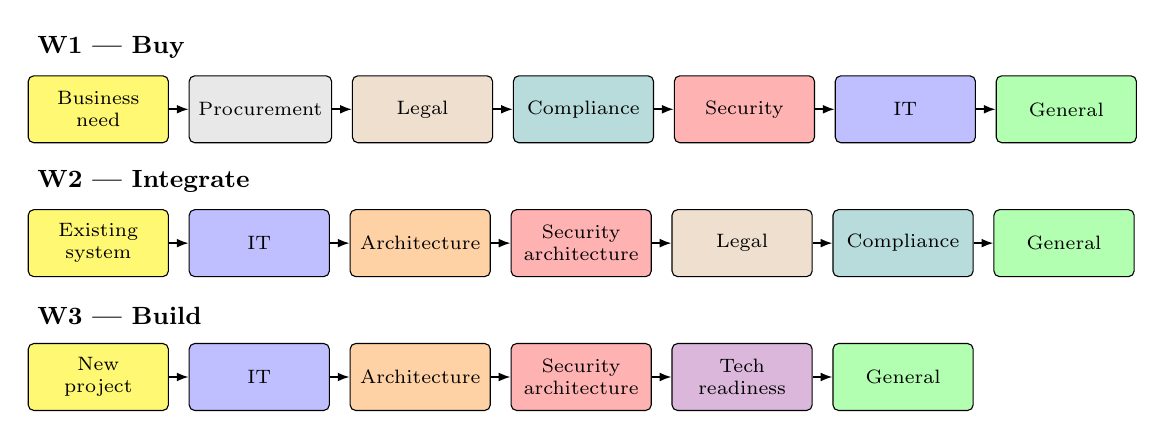
\begin{tikzpicture}[
  box/.style={draw, rounded corners=2pt, minimum width=1.78cm, minimum height=0.85cm,
              align=center, font=\scriptsize},
  arr/.style={-{Latex[length=1.5mm]}, semithick}, node distance=0.25cm]
\node[anchor=west, font=\small\bfseries] at (0,0.78) {W1 --- Buy};
\node[box, fill=yellow!55, anchor=west] (a0) at (0,0) {Business\\need};
\node[box, fill=gray!18, right=of a0] (a1) {Procurement};
\node[box, fill=brown!25, right=of a1] (a2) {Legal};
\node[box, fill=teal!28, right=of a2] (a3) {Compliance};
\node[box, fill=red!30, right=of a3] (a4) {Security};
\node[box, fill=blue!25, right=of a4] (a5) {IT};
\node[box, fill=green!30, right=of a5] (a6) {General};
\foreach \i/\j in {a0/a1,a1/a2,a2/a3,a3/a4,a4/a5,a5/a6} \draw[arr] (\i)--(\j);

\node[anchor=west, font=\small\bfseries] at (0,-0.92) {W2 --- Integrate};
\node[box, fill=yellow!55, anchor=west] (b0) at (0,-1.7) {Existing\\system};
\node[box, fill=blue!25, right=of b0] (b1) {IT};
\node[box, fill=orange!35, right=of b1] (b2) {Architecture};
\node[box, fill=red!30, right=of b2] (b3) {Security\\architecture};
\node[box, fill=brown!25, right=of b3] (b4) {Legal};
\node[box, fill=teal!28, right=of b4] (b5) {Compliance};
\node[box, fill=green!30, right=of b5] (b6) {General};
\foreach \i/\j in {b0/b1,b1/b2,b2/b3,b3/b4,b4/b5,b5/b6} \draw[arr] (\i)--(\j);

\node[anchor=west, font=\small\bfseries] at (0,-2.62) {W3 --- Build};
\node[box, fill=yellow!55, anchor=west] (c0) at (0,-3.4) {New\\project};
\node[box, fill=blue!25, right=of c0] (c1) {IT};
\node[box, fill=orange!35, right=of c1] (c2) {Architecture};
\node[box, fill=red!30, right=of c2] (c3) {Security\\architecture};
\node[box, fill=violet!28, right=of c3] (c4) {Tech\\readiness};
\node[box, fill=green!30, right=of c4] (c5) {General};
\foreach \i/\j in {c0/c1,c1/c2,c2/c3,c3/c4,c4/c5} \draw[arr] (\i)--(\j);
\end{tikzpicture}
\caption{\textbf{Three generic DGF routes, one illustrative configuration.} Yellow: initiating need or
event; grey: Procurement; brown: Legal; teal: Compliance; red: Security, a supplier security review in Buy and Security architecture elsewhere; orange:
Architecture; blue: IT; purple: Tech readiness; green: General gate. Colors identify gate types, not
automation maturity. Each route mobilizes a different subset of the eight gate types of
Table~\ref{tab:gates}, in a different order, and ends at the general gate. Enterprises define their own
gates, orders, and tasks.}
\label{fig:workflows}
\end{figure}

The triggering need, system, or project is not another approval gate. In Buy, the supplier's own
contribution, its proposal, evidence, and commitments, enters through Procurement; it belongs to another
organization and cannot be removed from an end-to-end automation analysis. In this configuration the
three routes contain seventeen gate occurrences after the trigger: six in Buy, six in Integrate, five
in Build. Every gate type appears at least once. The sponsors' commitment is recorded at the general
gate; it is not drawn as a separate box.

The order differs for a reason in each example. Buy examines the supplier's commitments, contract, data
obligations, and security before the run model is fixed; its security gate is a supplier security review,
and no dedicated Architecture gate is mobilized: architects are consulted on integration and data flows
without a gate of their own. Integrate starts from
what exists: IT inventories the inherited system before Architecture and Security assess it, and Legal
and Compliance then qualify the inherited obligations. Build starts by asking whether a solution
already exists in the catalog, and adds a Tech readiness review before production. These orders are
examples (Section~\ref{sec:notfixed}): the enterprise chooses its gates and their order, and what the
law requires is that automation preserve that choice, not these particular routes.

The figure shows nominal forward paths. Reservations, rework, suspension, evidence requests, and dated
conditions remain part of execution, and several gates can review one shared dossier in parallel.
An implementation that always approves, or always refuses to avoid hard cases, fails the function. Full
automation preserves substantive decision quality and the permitted control flow, not just the order of
labels. The same label can also describe different context-sensitive transformations: the security gate in Buy evaluates a supplier's package and commitments; in Integrate, Security
architecture evaluates an inherited system already scoped by IT.

\section{A gate is a contract, not a profession}
\label{sec:contract}

\begin{definition}[Gate-centered work package]
A work package $G_{w,j}$ is the preparation, inquiry, evaluation, decision production, authorized
action, and handoff surrounding position $j$ of route $w$. For versioned state $S$, accessible evidence
$E$, and policies $\Pi$,
\begin{equation}
(S^{+}, D, U) = G_{w,j}(S, E; \Pi, w), \label{eq:gate}
\end{equation}
where $D$ is a disposition and $U$ an action/evidence trace. The procedure may be interactive and
stochastic.
\end{definition}

The input includes more than a PDF: architecture records, observations obtained through tools, a
supplier's reply, costs, identities, outstanding conditions, and a history of negotiations. Requesting
missing evidence is part of the transformation. The output includes more than prose: it can create a
ticket, block a connection, require a redesign, approve a bounded action, or record a refusal. A valid
negative decision is an output; an unsupported declaration that an absent report was verified is not.
Authorization makes an eligible disposition effective; producing it does not confer that authority.

A contract $C_{w,j}$ specifies admissible input histories, acceptable output and action relations,
evidence obligations, quality tolerances, and authority. Several decisions may be defensible. A
replacement need not reproduce a particular person's wording, but it must meet the accepted decision
standard. The reference standard also records disputed judgments instead of treating every historic
human decision as ground truth.

\begin{definition}[Replacement of gate execution]
An implementation replaces a gate when it satisfies $C_{w,j}$ without requiring a person to complete
its ordinary work, exceptions, verification, or per-case authorization. Human participation that
remains necessary is counted as residual execution labor, whether performed internally, by a
contractor, or behind an apparently autonomous service.
\end{definition}

This distinction is established organizational practice, not a newly discovered property of
computation. Stage-Gate separates the work performed in stages from gates that evaluate deliverables, apply
criteria, and decide whether a project proceeds, waits, stops, or returns for further work
\citep[p.~46]{cooper1990}; artifact-centered process modeling represents the records transformed by
business operations \citep{nigam2003}. These antecedents support implementation neutrality. They do
not by themselves prove that every information contract is computable, sufficiently observable,
economically executable, or legally delegable; Sections~\ref{sec:candidate}
and~\ref{sec:premises} give the reasons to expect it for the DGF.

\subsection{Three conditions for complete execution}
\label{sec:conditions}

For a declared case population and contract version, complete execution has three simultaneous
conditions. \emph{Labor:} no necessary human time on any admitted visit, including exceptions and
per-case authorization. \emph{Quality:} independently adjudicated performance satisfies prespecified
noninferiority margins against the human reference and absolute limits on consequential errors, false
refusals, information leakage, and delay. \emph{Mandate:} the decision is institutionally effective,
not merely a recommendation.

A sample containing no human interventions supports, but cannot prove, zero intervention on every
future input. Operational evidence must therefore combine time records, tests, and an architecture
with no required manual step. Assessment by researchers does not itself make operation manual; any
continuing human assessment required to keep the service qualified does count as support. The
distinction is functional, not organizational. A service with autonomous visits but a human
maintenance team has achieved execution closure, not support closure. Initial development is recorded
as a transition investment; continuing updates, incident response, mandated oversight, and outsourced
verification cannot disappear from the account because they have moved to a supplier.

\subsection{One handoff contract and four operating stages}
\label{sec:stages}

A supplier contract can reach Legal as a PDF, Security as an email attachment, and IT production as a
project-manager summary. Each function then extracts the supplier, hosting locations, security
commitments, unresolved clauses, and evidence expiry dates. The interface gain is to perform this
extraction once and attach a provenance trail that the other functions can inspect. The minimal
reusable record contains case and source version, route and gate, claim, evidence locator, verification
status, action owner, risk owner, deadline, and authorization reference:
\par\noindent\begin{minipage}{\linewidth}
\begin{lstlisting}
route: W3
current_gate: TECH_READINESS
recommendation: NOT_READY
claim: load_test_incomplete_and_restoration_not_tested
evidence: {reference: restore-test-report, status: missing}
action_owner_role: production_lead
risk_owner_role: business_service_owner
approval_reference: null
execution_authorized: false
next_action: run_restoration_test_or_request_authorized_exception
\end{lstlisting}
\end{minipage}\par
The record is a schema illustration. Its empty approval reference blocks authorization. A field
marked missing carries information; replacing it with an invented value destroys that information.
This is the difference between a local copilot and a connected process: a copilot saves one reviewer's
reading time, whereas a dependable evidence object changes the work of several downstream functions. A
human can also create that object, which is why Section~\ref{sec:testing} separates the value of
structure from the value of agentic production.

In a \textbf{human pipeline}, specialists prepare and check every dossier. In an \textbf{assisted
pipeline}, agents collect or draft while humans inspect the ordinary path. In an
\textbf{exception-routed pipeline}, eligible work executes automatically, while experts handle
exceptions, sampled review, and retained authorizations. The thesis adds a fourth stage, the
\textbf{closed pipeline}, in which exceptions, verification, and authorization are executed under
mandate as well. The configurations can coexist within a route, and no company is assumed to move
monotonically: incidents can restore manual review. The transition moves the expert from reviewing every ordinary case to governing the system that
reviews them (Section~\ref{sec:implications}), until those tasks are themselves executed by software.

\section{Every role has the same shape: documents in, an artifact out}
\label{sec:roles}

Whatever the role, the work of a DGF has one shape. The input is a set of documents and records that
an agent can read: a design, a diagram, a contract, a test report, a register of findings. The output
is an artifact that an agent can write: an opinion, a list of findings, a redlined clause, a readiness
verdict, a risk card, a decision record. A security architect reviewing an architecture diagram, a
readiness expert reviewing a recovery, resilience, and backup dossier, and a GRC expert proposing a
risk card perform the same kind of transformation. What differs between them is the policy applied
and the evidence required, not the form of the work. Table~\ref{tab:roles} states that shape for every
population and for the general gate.

\begin{table}[!htb]
\centering\small\renewcommand{\arraystretch}{1.18}
\caption{Documents in, artifact out: the input each role reads and the output it returns.}
\label{tab:roles}
\begin{tabularx}{\linewidth}{@{}P{3.3cm}LL@{}}
\toprule
Role & Input the agent can read & Output the agent can return\\
\midrule
Procurement (R1) & Business need, vendor proposals, price lists, supplier questionnaire. & Supplier
comparison, normalized commercial terms, sourcing recommendation, contract draft.\\
Legal / Contracts (R2) & Contract draft, data-processing agreement, SLA and security annexes,
subprocessor list. & Redlined clauses, accepted and rejected terms, legal exceptions, obligations
register.\\
Architecture (R3) & Requirements, high-level and detailed architecture, integration and flow diagrams,
network matrix. & Architecture opinion, integration pattern, network conditions, recorded decisions and
waivers.\\
Security Architecture (R4) & Architecture diagram, flow matrix, data classification, identity and
access model, supplier evidence. & Findings with severity, required controls, risk scenarios, opinion.\\
Compliance / Privacy / GRC (R5) & Data categories, purposes, processors and locations, control assessments, gate
findings. & Assessment requirements, transfer and retention conditions, risk card with owner and
treatment.\\
IT Production and Standards (R6) & Catalog conformity sheet, licence inventory, operations dossier,
support model. & Conformity opinion, waivers with a convergence plan, run
acceptance.\\
Tech Readiness (R7) & Pilot, load-test, and code-quality results; recovery, resilience, and backup
dossier: backup policy, restoration test report, recovery objectives, runbooks. & Readiness verdict,
open conditions, retest dates.\\
General Gate Support (R8) & Gate opinions, reservations register, schedule, risk cards, residual risks.
& Consolidated gate dossier, dated action plan, acceptance package.\\
Finance / Cost Control (R9) & Solution design, usage assumptions, quotes, budget envelope. & Budget
opinion, cost guardrails, variance alerts.\\
General gate (committee and sponsors) & Gate dossier, opinions, residual risks, budget, schedule. &
Recorded decision: go, go with reservations, rework, suspension, or no-go, with owners, dates, and the
sponsors' commitment.\\
\bottomrule
\end{tabularx}
\end{table}

The three worked routes of Section~\ref{sec:routes-worked} come from a security practitioner's
framework, so their blocking findings are security findings. Table~\ref{tab:rolecases} therefore adds
eight examples, one per gate type of Table~\ref{tab:gates}, in which the blocking finding arises at a
different gate each time. They are illustrative examples written for this paper, not cases from the
framework.

\begin{table}[!htb]
\centering\footnotesize\renewcommand{\arraystretch}{1.15}
\caption{Eight illustrative reviews, one per gate type. In each, the expert reads documents and returns
an artifact; nothing in the transformation requires that the reader be a person.}
\label{tab:rolecases}
\begin{tabularx}{\linewidth}{@{}P{2.4cm}P{3.5cm}LL@{}}
\toprule
Gate and role & Documents read & Blocking finding & Artifact returned\\
\midrule
General: portfolio committee & Gate dossier: opinions of the specialized gates, risk cards, updated
business case, budget, schedule. & Cost above the approved envelope and one reservation still open, while
the business asks to proceed. & Recorded decision: go with reservations under a budget cap, a named risk
owner, and a review date, or no-go.\\
IT: production and standards lead & Catalog conformity sheet, licence inventory, operations dossier,
support model. & Database engine outside the catalog and out of vendor support; no on-call model defined.
& Opinion with reservations: waiver request with a convergence plan; support model required before
the change advisory board.\\
Architecture: enterprise architect & High-level architecture, flow diagram, interface list, network
matrix. & Point-to-point file transfer bypassing the integration platform; inter-site bandwidth
insufficient for nightly volumes. & Architecture decision record: required integration pattern, network
sizing condition, waiver recorded with a remediation date.\\
Security architecture: security architect & Architecture diagram, flow matrix, data classification. &
Administration interface exposed to the internet; unencrypted flow carrying confidential data. &
Findings with severity, required controls, unfavorable opinion or opinion with reservations.\\
Tech readiness: readiness expert & Pilot and load-test results, code-quality report, recovery,
resilience, and backup dossier, runbooks. & Load test stopped at half the target volume; last restoration
test older than twelve months. & Not-ready verdict, tests requested with dates, handover blocked until
the evidence is attached.\\
Procurement: buyer & Need statement, supplier proposals, pricing grids, third-party due-diligence report.
& Lowest bid has the highest total cost once licences and exit costs are counted; one supplier fails
financial due diligence. & Multi-criteria scoring, sourcing recommendation, negotiation points for the
commitment committee.\\
Legal: contract lawyer & Supplier contract, data-processing agreement, service-level annex. & Liability
cap below policy; no audit right; subprocessor change without notice. & Redlined clauses, legal
exceptions with positions, obligations register for the supplier file.\\
Compliance: GRC expert & Gate findings, control assessment, processing description, applicable
regulations. & Residual risk above tolerance after the proposed controls; impact assessment missing for a
new processing of personal data. & Risk card: scenario, impact and likelihood classes, score, treatment
options, proposed risk owner, acceptance record to be signed; impact assessment required.\\
\bottomrule
\end{tabularx}
\end{table}

Three remarks follow. First, when a document is missing or insufficient, the output is a request for
evidence, an unresolved status, or a refusal; that is still an artifact, and producing it is part of the
contract of Definition~1. Second, some inputs are obtained rather than received: a restoration test is
launched, a supplier is asked, a configuration is queried. Those are actions an agent can take through
tools, within its mandate. Third, the artifact of one role is the document of the next: the
IT opinion is read by Architecture and Security, the findings are read by Compliance, the risk card is read
by the committee, the decision
is read by the sponsors. A DGF is a chain of documents read and artifacts returned, which is the form
of work that agents already perform. This is the practical content of Law~1.

The shape of the work is not a proof that all its requirements can be executed. Two situations that
look identical in the accessible documents can require different decisions; no reader, human or
machine, can then decide correctly without further inquiry (Appendix~\ref{app:limits}). The shape says
where inquiry must go and what must be returned; whether every requirement can be met without a person
is what the hypotheses of Section~\ref{sec:hypotheses} test.

\section{Why the DGF is the most likely first candidate for agentic automation}
\label{sec:candidate}

Alongside the law, we state a separate comparative hypothesis: \textbf{among the expert control
functions of an enterprise, the DGF will be the first to be completely executed by agents.} The law
does not depend on it; the DGF could close after another function and the law would still hold. The
hypothesis rests on seven properties that few other functions combine.

\textbf{Its objects are already digital.} A DGF reviews software systems, configurations, contracts,
evidence, and institutional commitments. Repositories, identity systems, cloud control planes, ticketing
tools, and APIs already supply most of the observations and actions a gate needs. Nothing has to be lifted, driven, or examined at a bedside: every role reads documents and returns an
artifact (Table~\ref{tab:roles}).

\textbf{It is already a paved road} (Section~\ref{sec:dgf}). The representation work that blocks
automation elsewhere has been done here for human reasons.

\textbf{Its decisions concern systems and projects.} An architecture approval is not a hiring, credit,
or medical decision about a person. This does not exempt it from law (Section~\ref{sec:mandate}), but it
places the DGF further from the strictest regimes on automated decisions than most candidate functions.

\textbf{It is a cost center and a bottleneck.} Review queues delay every project of the enterprise. An internal review is not
a product feature: customers buy the firm's products, not the identity of whoever performed its
internal reviews. Where a contract or a regulator does require a named human reviewer, that is an
institutional constraint of the kind discussed in Section~\ref{sec:mandate}, not a commercial
preference. Management therefore faces both a speed incentive and a cost incentive.

\textbf{Its work is specialist work, and much of it is repetition.} The same facts are extracted from the
same documents by Procurement, Legal, Security, and IT production. How many visits are standard is an empirical frequency, measurable on historical logs. Hypothesis~H3
makes a separate prediction: the residual holds a larger share of the hours than of the cases
(Section~\ref{sec:selection}), whether or not standard cases are the majority.

\textbf{Its outputs are checkable downstream.} A condition such as ``EDR before interconnection'' or
``log export in the contract'' can be verified by the next gate or by the production system itself. A
function whose outputs can be tested is a function whose automated executor can be qualified.

\textbf{Its neighbors are already software.} Bounded governance decisions around the DGF already execute
without a fresh human judgment (Table~\ref{tab:precedents}).

The comparison class matters. Transactional back-office functions, such as invoice processing, order
creation, post-trade matching, and first-level service desks, are already largely executed by software;
they are the precedents of Section~\ref{sec:precedents}, not rivals for this hypothesis. The rivals are
the other expert control functions staffed by senior specialists: legal review, financial control and
audit, credit and underwriting decisions, human-resources decisions, clinical review. The criterion is
execution closure as defined in Section~\ref{sec:conditions}, reached for every gate of the function at
a participating site. Human-resources, credit, and clinical decisions concern persons and meet the
strictest legal regimes; legal work carries privilege and professional liability; audit is bound by
independence rules. The DGF combines high structure, digital evidence, internal impact, and management
pressure. The hypothesis fails if another expert control function reaches execution closure first. On
this hypothesis, the populations of Table~\ref{tab:populations} are the first specialist workforce
exposed.

\section{Why believe complete automation will extend to every gate?}
\label{sec:premises}

The argument is inductive and compositional, rather than a deduction from notation.
Table~\ref{tab:premises} distinguishes evidence already available from the extension that the thesis
needs.

\begin{table}[!htb]
\centering\small
\caption{Five premises, with their evidential boundary. The final column contains the substantive
burden of the complete-automation thesis.}
\label{tab:premises}
\begin{tabularx}{\linewidth}{@{}P{3.0cm}LL@{}}
\toprule
Premise & Evidence or mechanism & Remaining claim to test\\
\midrule
Contract, not occupation & Each DGF specifies evidence, criteria, outputs, and the order chosen for its
routes. & Contracts
capture material inquiry and judgment without concealing a necessary human.\\
Capability reaches gate scale & Measured software-task horizons have increased substantially. &
Comparable progress transfers to messy gate work and the required reliability tail.\\
Gates already become software & CI quality rules, cloud policy, standard changes, and transaction
processing execute bounded controls. & Automation extends from these controls to the full judgment and
exception loop.\\
Authority becomes a mandate & Authorized rules can release changes or orders without another per-case
decision. & Required commitments can be validly delegated on each DGF route.\\
Provision scales & Reusable services can spread common engineering and assurance costs. & Local
adaptation and risk costs do not preserve an economic or human-support floor.\\
\bottomrule
\end{tabularx}
\end{table}

\subsection{Capability is moving toward longer coherent work}
\label{sec:capability}

\citet{kwa2025} introduce a task-completion horizon measured in human expert time, not in the agent's
runtime. Their 2019--2025 results show an approximately seven-month doubling of the 50\% horizon on
software-related tasks, and a similar trend for the 80\% horizon at roughly one fifth of the length.
They associate the increase with better reliability, error recovery, reasoning, and tool use. This is
the strongest measured trend supporting the move from individual instructions to extended work
packages.

The later METR dashboard, updated on 8 May 2026, reports for its best-performing model a 50\% horizon
of at least sixteen hours, with a 95\% interval of 8.5--55 hours, and warns that measurements above
sixteen hours exceed the reliable range of its task suite \citep{metr2026a}. The reported point is not
a guarantee that every sixteen-hour activity can be completed.

The inference to gates requires care. A twelve-, twenty-four-, or thirty-six-hour dossier can contain
parallel work by several specialists; it is not automatically one coherent task of that duration. The
12--36-hour examples below are synthetic reference workloads, not measured DGF horizons. METR's tasks
are mainly self-contained software engineering, machine-learning, and cybersecurity problems; its
documentation emphasizes domain variation over orders of magnitude, low-context human baselines, worse
transfer to messy work, and error bars of roughly a factor of two \citep{metr2026a,metr2026b}. It does
not estimate 99\% horizons.

These qualifications change how the evidence is used, not its relevance. A trend from short tasks to
multi-hour, tool-using work is evidence against a fixed boundary at a document summary. The thesis is
that the same combination of improved reasoning, access, recovery, and verification closes the larger
contracts. Sections~\ref{sec:milestones} and~\ref{sec:testing} expose the additional assumptions and
tests.

\subsection{The inductive precedent: some decisions already run as software}
\label{sec:precedents}

Table~\ref{tab:precedents} documents operational mechanisms in the same organizational neighborhood as
the DGF. The important observation is not a vendor's adoption claim. It is that an input can already be
checked against an authorized condition and cause an effective action without a fresh human judgment
in that bounded case.

\begin{table}[!htb]
\centering\small
\caption{Existing automation near the gate boundary. Documentation supports the stated mechanism,
without implying zero supporting labor or full automation of the wider function.}
\label{tab:precedents}
\begin{tabularx}{\linewidth}{@{}P{3.3cm}LL@{}}
\toprule
Primary example & Software-executed transformation & Boundary of the precedent\\
\midrule
CI/CD quality gates \citep{sonar2026} & Code-analysis measurements and conditions produce pass/fail;
pipeline or merge policy can enforce the result. & Encoded quality criteria, not every design or
security judgment.\\
Cloud policy-as-code \citep{mspolicy2025} & A resource request matching a deny policy is rejected
before resource-provider execution. & Enforces a rule; does not establish that the rule covers all
risks.\\
Standard changes \citep{atlassian2026} & A repeatable, documented, low-risk change can be
pre-authorized rather than approved anew. & Preauthorization supplies the mandate; automated execution
still needs an implementation.\\
Continuous deployment \citep{awscd2026} & A qualifying change proceeds automatically into production,
unlike delivery awaiting explicit release approval. & Tests, configuration, rollback, and supporting
operations remain relevant.\\
Touchless purchasing \citep{oracle2026} & An approved requisition can become a purchase order and be
communicated without a procurement agent's intervention. & Requisition approval and agreement formation
are prior inputs, not shown to be autonomous.\\
Compliance evidence \citep{awsaudit2026} & Service data are collected and associated with control
evidence. & The service explicitly does not assess compliance itself.\\
Post-trade processing \citep{dtcc2026} & Matching enables automatic trade affirmation and downstream
processing. & A bounded post-trade path, not the entire back office or all exceptions.\\
Automated underwriting \citep{fanniemae2026} & Application and credit information produce a risk
assessment and recommendation. & The lender retains underwriting judgment and responsibility.\\
\bottomrule
\end{tabularx}
\end{table}

These precedents refute the proposition that a governance-related decision necessarily requires an
employee to handle every instance. Some implement the decision itself; others automate evidence or
recommend an outcome while retaining a human. That contrast is useful: it identifies which part of the
contract remains open instead of labelling every use of software a completed gate.

The next step is therefore an extension, not a new direction of history. Deterministic controls
already translate accepted requirements into executable tests. Agents add interpretation, evidence
pursuit, exception diagnosis, and revision of a proposed plan. The favorable induction is that a
growing composition of such operations replaces the whole gate. Its strongest rival is that
unstructured judgment or assurance remains an irreducible last task. Section~\ref{sec:objections} tests
that rival rather than assuming it away.

\subsection{From an individual signature to a standing mandate}
\label{sec:mandate}

Authorization is not the same as a handwriting event. Continuous deployment and touchless order
creation illustrate execution under rules and prior approvals \citep{awscd2026,oracle2026}. A DGF can
similarly move an eligible class of decisions from repeated individual approval to a standing
delegation. The delegation specifies case class, allowed actions, budget and risk limits, evidence
requirements, expiry, suspension, and the principal on whose behalf the system acts.

At the general gate, the go decision and the sponsors' commitment are then a recorded, valid exercise of
that mandate. The gate remains and the commitment is effective; no person is impersonated and no machine declares itself a corporate officer. Cases
outside the mandate remain unresolved or are refused under the contract. A mandate with a required
human exception path has only partially automated the gate; its extension to every case class is part
of the thesis.

The legal limit is substantive. NIS2 Article~20 requires management bodies to approve and oversee
cybersecurity risk-management measures and addresses their liability and training. DORA Article~5
assigns management bodies responsibility for the ICT risk-management framework; Article~6(10) permits
outsourcing verification tasks while retaining the financial entity's responsibility
\citep{nis2,dora}. These texts support distinguishing execution from responsibility, but do not
authorize eliminating all human governance. Required continuing board work belongs in $B_A$. Under a
regime that retains it, a zero-support claim for that broad boundary fails unless the requirement
itself validly changes.

Nor is ``a decision about systems'' a general exemption. GDPR Article~22 concerns solely automated
decisions about people with legal or similarly significant effects, subject to specified exceptions and
safeguards; ordinary architecture approval is not automatically such a decision, but a DGF service can
affect access, employment, or other protected interests \citep{gdpr}. The AI Act's high-risk
classification and human-oversight provisions also depend on intended use and applicable conditions,
not the label DGF \citep[Arts.~6, 14 and Annex~III]{aiact}. Jurisdiction, national implementation,
effective dates, and sector rules must be assessed for the actual service. No legal opinion or
universal permission is asserted here.

The argument for migration is thus operational: the authorized principal can define a class-level rule
and let software execute it. The argument against complete support closure is institutional: some
continuing human obligations may survive that migration. Both are observable. Maintaining this
distinction strengthens the automation thesis by identifying what must change, rather than treating
liability as either a magical human advantage or an irrelevant detail.

\subsection{Shared provision can make a low-volume route economical}
\label{sec:provision}

A five-visit Integrate route may be uneconomic when it must build and maintain its own agent
platform. That does not imply that it remains uneconomic when buying a common service. Let $F_s$ be
fixed, shareable nonlabor platform cost, $N$ comparable customers, $F_c$ customer-specific fixed cost,
$a$ variable nonlabor cost per visit, and $\lambda_c$ visits at customer $c$. Under an equal allocation
convention,
\begin{equation}
\bar c_{c,\mathrm{platform}} = a + \frac{F_s/N + F_c}{\lambda_c}. \label{eq:platformcost}
\end{equation}
The common term falls with scale, while local integration does not. Falling provider cost reaches the
customer only if pricing passes through some of the saving. The same distinction applies to human
upkeep. Allocating shared hours $B_s$ and customer-specific hours $B_c$ gives
\begin{equation}
b_{A,c} = \frac{B_s/N + B_c}{\lambda_c h_{0,c}}. \label{eq:sharedupkeep}
\end{equation}

\begin{table}[!htb]
\centering\small
\caption{Synthetic low-volume provision: 60 common human upkeep hours per month plus six
customer-specific hours, five visits per customer, and 24 baseline hours per visit. Provider labor has
not disappeared; it is allocated explicitly.}
\label{tab:provision}
\begin{tabular}{@{}r r r r r@{}}
\toprule
Customers & Support hours/month/customer & Support hours/visit & Total hours/visit & $\rho$\\
\midrule
\rowsinput{generated/table_provision_rows}
\bottomrule
\end{tabular}
\end{table}

Table~\ref{tab:provision} applies Equation~\eqref{eq:sharedupkeep} to the five-visit Integrate route of
Section~\ref{sec:routes}, whose direct residual effort is 21.62 hours per visit. Alone, the customer
faces a workload ratio of 1.451; sharing the sixty common hours across 1,000 customers while keeping
all six local hours lowers it to 0.951. The verdict on a low-volume route therefore turns on
whether it must carry its own policies, tests, and evaluations or can share them. The table holds the
sixty common hours constant as customers are added, which is the favorable case: the empirical
question is whether shared support hours grow less than proportionally with the number of customers.

Amortization lowers a buyer's allocated burden; it does not eliminate the provider's workers. Across
all customers the shared hours still sum to $B_s$, and the local hours to $\sum_c B_c$. Full support
closure requires automating or removing the required work itself. Economies of scale make the
investment plausible; they are not a shortcut to zero global labor.

\section{The law of gate substitution: statement, five component laws, six path hypotheses}
\label{sec:law}

\noindent\fbox{\begin{minipage}{\dimexpr\linewidth-2\fboxsep-2\fboxrule\relax}
\textbf{The law of gate substitution.} Every gate-centered work package that an
enterprise places in its DGF, whatever gates it has chosen, obtains, and moves to, an effective automated implementation of its accepted input-output
contract. Inquiry, exceptional-case analysis, verification, the general gate's arbitration, and the commitment it
records are included.
The recurring work needed to operate and verify those implementations is itself a substitution
target, not a permanently human role. At fixed governed output, the human workforce required to
execute the DGF contracts toward its remaining support floor, and then toward zero.

\smallskip\emph{Status: a conjecture proposed by the author, not an established result. Its ten-year
cohort form (Section~\ref{sec:testing}) can be refuted.}
\end{minipage}}

\medskip
``Every gate'' is a universal claim over gate types and their declared case domains. It is not a claim
that a machine will know an unobserved fact, that every judgment is error-free, or that all enterprises
cross the boundary on the same date. The accepted quality specification stays fixed while
implementations are compared; the thesis does not make the specification easier by removing difficult
cases. Its technical and adoption components are separately observable: a qualifying implementation
exists, and the organization actually uses it under a valid mandate.

\subsection{Five component laws}

The five laws name distinct commitments of the thesis.

\law{Law 1}{Contract substitutability}{A DGF gate's function is specified by the transformation it
performs, not by the profession that currently staffs it.} Operational contracts, augmented with
inquiry and action interfaces, capture enough of that function to support an implementation-independent
evaluation. It fails for a stated domain if a material part of successful execution cannot be
represented or evaluated without an indispensable personal intervention.

\law{Law 2}{Complete execution}{No DGF gate class is a permanent exception to autonomous execution.}
Progressively broader implementations ultimately cover the entire gate, rather than stopping at a
permanently human layer of difficult decisions. A durable technical or institutional requirement for
human execution in one gate class contradicts its strong form.

\law{Law 3}{Route preservation}{Replacing the execution of every component replaces the execution of
the route without erasing its required gates.} Replacements preserve the composition the enterprise has decided: its gates, their order on each route,
their conditions, and their returns. Gates are interchangeable for the enterprise that composes the
DGF, which can add, remove, merge, or reorder them at any time; they are not interchangeable for the
agent that executes it. What is preserved is every obligation and the logical order of authorizations,
not the physical existence of each box: one service can execute several contracts, but dropping or
reordering a required control to make automation easier is not its replacement.

\law{Law 4}{Execution displacement}{For a fixed amount of governed work, automating the complete route
removes the labor demand that staffed its execution.} The reduction is not merely a change in job
descriptions. It follows when removed execution work is not replaced by equally large required human
support (Section~\ref{sec:workforce}).

\law{Law 5}{Supervisory closure}{Monitoring, exception review, policy maintenance, and verification are
additional transformations to automate, not permanent human refuges assumed by definition.} If they
remain labor-intensive, the system is only partially closed.

\subsection{What makes the law stronger than an augmentation claim}

An augmentation claim permits the same human team to remain indispensable while using better tools.
Complete substitution does not. A staff member who must interpret every output, reconstruct every rare
incident, or sign every individual approval is still executing part of the gate. Reducing the average
time of that intervention is progress toward substitution, not completion of it. Likewise, the future
workload is not assumed to consist only of easy cases. When an exception becomes a named subprocedure,
the thesis treats that subprocedure as a new target for the same input-output analysis. An
indefinitely expanding collection of indispensable human subprocedures would defeat the strong
endpoint, even if each software release automates more standard cases.

\subsection{Six hypotheses about the path}
\label{sec:hypotheses}

The component laws state the destination. Six hypotheses describe the transition and can be tested
long before the endpoint. Each predicts an observable pattern and can fail within a specified case
population. Automation is evaluated against independently assessed quality, not merely whether a
workflow reaches an approval state.

\law{H1}{Gate readiness}{Gate-level readiness improves out-of-sample prediction of reliable automation
beyond model capability and case length.} Accessible inputs, explicit criteria, independent evidence
checks, scoped actions, and testable outcomes explain differences between otherwise comparable gate
implementations (Appendix~\ref{app:readiness}).
\failure{Failure criterion:} prospectively scored readiness provides no reproducible predictive
improvement over case-size, duration, and evidence-completeness baselines, or repeatedly assigns high
readiness to unresolvable critical failures.

\law{H2}{Handoff propagation}{2a: Evidence-bearing, structured handoffs reduce total human work across
the connected process.} Production, verification, reconciliation, and repeat work all enter the
endpoint; the predicted format contrast is $\beta^{(h)}_{F}<0$ for total hours
(Section~\ref{sec:testing}). \textbf{2b: At equivalent downstream benefit and quality, agents produce
and verify the structured handoff at lower resource cost than humans.} The agent contrast is
$\beta^{(c)}_{A}+\beta^{(c)}_{AF}<0$ for upstream production-and-verification cost. This is the
specifically agentic increment, separate from the value of structure.
\failure{Failure criteria:} 2a fails without lower total hours; 2b fails without lower upstream cost
and equivalent downstream benefit and quality. Both comparisons retain all assigned cases, including
rejected artifacts and work transferred upstream.

\law{H3}{Labor concentration in the human residual}{As agents absorb the standard path, residual cases
retain a larger fraction of baseline labor than their fraction of case volume.} A small human queue
can therefore contain a large share of the work. The prediction concerns baseline effort measured
before deployment, not a difficulty score defined after observing the routing decision.
\failure{Failure criterion:} the residual does not become enriched in baseline effort under the tested
standard-case rollout, or this pattern disappears across held-out case classes. Random-audit and
mandatory-signature queues provide comparison groups.

\law{H4}{Residual workload prediction}{Exception-adjusted forecasts predict human-capacity change
better than the uniform-effort model $q+(1-q)m$.} The comparator gives every exception the baseline
average effort and sets review to fraction $m$ of that average. The component model additionally represents baseline selection, post-deployment exception effort,
rework, and recurring human upkeep. Beating a comparator that omits hours actually worked would prove
little, so a second comparator receives the same rework and upkeep hours and the directly estimated
conditional means $h_E$ and $h_R$. With coherent inputs it is algebraically identical to the component
model; the separation of $\kappa$ from $\eta$ earns its keep only when the routing rule, the case mix,
or the agent configuration changes, because $\phi$ can then be re-estimated on historical work while
$\eta$ and $\mu$ are carried over. H4 therefore tests a transferability hypothesis: that effort ratios
carry over to new conditions better than conditional hours do. It is plausible where assistance scales
with the baseline difficulty of a case, and doubtful where it helps some categories of exception much
more than others, since a change of mix then changes the average $\eta$ without any change in the
agent.
\failure{Failure criterion:} using prospectively estimated inputs, the component model does not
improve held-out total-hours forecasts over the uniform comparator and a stratified case-mix baseline,
does not beat the matched comparator after a change of routing, mix, or configuration, or exceeds a
prespecified error tolerance.

\law{H5}{Delegation before authorization}{At consequential gates, delegation of analytical production
advances ahead of delegation of final authorization.} The enterprise changes who prepares and executes
a decision before changing who is empowered to approve it and answer for its consequences. H5
describes the \emph{order} of the transition; Law~2 states its endpoint.
\failure{Failure criterion:} analysis and authorization transfer at the same rate, or authorization
transfers earlier, in settings where both can vary. A universal human-signature mandate explains a
fixed boundary but cannot by itself validate the prediction. The lag is an institutional outcome to
measure, not a claim about a uniquely human cognitive capability \citep{novelli2024}.

\law{H6}{Residual exhaustion}{The set of indispensable human interventions shrinks toward empty:
categories of intervention close faster than new ones appear, including those created by supervising
the agents.} H1--H5 can all hold while a small team remains indispensable. Three propositions of increasing strength
must not be confused: one human intervention can be automated; the remaining interventions become
automatable one after another; and there is a date after which no necessary human intervention remains.
The law needs the third. H6 is the hypothesis that separates complete substitution from durable
complementarity. Each remaining intervention is recorded
by category and by origin: present at baseline, displaced from another role or organization, or created
by the automation itself.
\failure{Failure criterion:} over three successive annual evaluations, the number of indispensable
intervention categories, or the hours they absorb, stops falling, or newly created categories offset those that close. Such a result rejects this trajectory
hypothesis; like the plateau of Section~\ref{sec:testing}, it is warning evidence for the endpoint, not
its refutation before the deadline.

\section{Three worked routes and their substitutable transformations}
\label{sec:routes-worked}

Each generic route is illustrated by one case from the practitioner framework. The initial situations
and the recorded opinions come from that framework; the route orders are the illustrative configuration
of Figure~\ref{fig:workflows} (Section~\ref{sec:notfixed}), and the proposed machine operations are the
implementation examined by the thesis. The cases are not reports of tested autonomous deployments.

\subsection{W1, Buy: a new platform, from supplier request to the general gate}

The framework's SaaS CRM serves 2,000 sales users and handles confidential customer data. It plans SSO
with optional MFA, lacks contractual SIEM log export, and has untested restoration with no defined
recovery-time objective. Its Security opinion is red, with log export to be negotiated before
signature and MFA and recovery conditions before go-live \citep[p.~103]{canale2026}. The same dossier
gives work to every gate: Procurement and Legal carry the negotiation of the log-export clause,
Compliance qualifies the customer data, IT checks the catalog fit and the run model, Finance validates the
cost, and the general gate arbitrates. The
Security opinion is one transformation among them.

\begin{table}[!htb]
\centering\small
\caption{W1, Buy, in the illustrative order. The proposed machine operations preserve the CRM case's
initial red opinion; they do not assert a later approval.}
\label{tab:w1}
\begin{tabularx}{\linewidth}{@{}P{2.7cm}LL@{}}
\toprule
Gate & Input & Output and automation target\\
\midrule
Procurement & Need, budget, requested controls, supplier proposals and evidence. & Sourcing questions,
offer comparison, evidence requests, due-diligence result.\\
Legal & Draft contract, service-level and data annexes. & Redlined clauses: log export, audit right,
liability, reversibility.\\
Compliance & Data categories, purposes, hosting locations. & Processing assessment, transfer and
retention conditions.\\
Security & Supplier security package, flows, identity model, classification. & Evidence-backed opinion;
contractual changes and preconditions, including the MFA and recovery conditions.\\
IT & Catalog, run and support model. & Catalog fit, run and support model, operating constraints.\\
General & Opinions, reservations, business case, budget, owners. & Go, go with reservations, rework, or
no-go, with owners and dates.\\
\bottomrule
\end{tabularx}
\end{table}

In this configuration the enterprise consults Security before the run model is fixed; automation must respect the order the enterprise has chosen and must not send a
technically integrated platform to Security after the fact. The reusable object is the evidence record of
Section~\ref{sec:stages}, here a contract with exact clause locators; Legal, Compliance, and Security
reuse it instead of re-extracting the same PDF. An automated red disposition is a \emph{successful}
execution of this example when the reference requirements still fail. Automatically producing a green
status would not be substitution; it would be degradation of the governance function. The supplier
belongs to another organization: buyer-side automation cannot hide the supplier's evidence-production
labor, and the complete claim for this route includes that interaction.

\subsection{W2, Integrate: an information system inherited from an acquisition}
\label{sec:cases-parameters}

The acquired entity has 400 people, its own on-premises Active Directory, cloud mail, and a
provider-hosted ERP. A payroll requirement motivates network interconnection within thirty days,
despite missing account inventories, no endpoint detection and response (EDR), local logs, and an
undocumented past incident \citep[p.~104]{canale2026}. IT first frames integration, isolation, or
retirement; Architecture and Security then assess that scope, Legal and Procurement recover the
inherited ERP obligations, Compliance qualifies the inherited data, the general gate's support staff
track the dated obligations, and Finance prices the integration options. The corporate acquisition
decision itself is outside this route.

\begin{table}[!htb]
\centering\small
\caption{W2, Integrate, in the illustrative order.}
\label{tab:w2}
\begin{tabularx}{\linewidth}{@{}P{2.7cm}LL@{}}
\toprule
Gate & Evidence received & Work, output, and automation target\\
\midrule
IT & Payroll need; inherited AD, mail, ERP; available inventories and provider documents. & Frame what
will be integrated, isolated, or retired; plan the run takeover; transmit scope, dependencies, and
explicit evidence gaps.\\
Architecture & IT scope, inherited flows and interfaces, network constraints. & Target integration
architecture; design of the restricted connection; conditions.\\
Security architecture & Scope; identity, exposure, incident, EDR, and logging evidence. & Assess
integration risk; carry the framework's conditional (yellow) opinion into a risk card, a restricted
connection scope, and dated control requirements.\\
Legal & Hosted ERP contract, inherited service obligations. & Obligations register; novation or exit
conditions.\\
Compliance & Inherited personal data, applicable rules. & Conditions on data access and retention.\\
General & Gate opinions, residual risks, integration owner, cost and schedule. & Record the decision and
its authorized scope, accepted residual risk, conditions, and follow-up; preserve the integration
director's risk ownership.\\
\bottomrule
\end{tabularx}
\end{table}

The framework's path overview prohibits interconnection before the acquisition audit. Its worked case
records a bounded exception: a filtered partner-zone connection during the audit without joining
directories, EDR before any connection, the account inventory within thirty days, SIEM log integration
within sixty days, and a risk card signed by the integration director; directories are joined only
after the audit \citep[pp.~18, 104]{canale2026}. These are different prerequisites and dated
obligations, not a blanket approval.

An agent can reconcile inventory exports, link accounts to owners, locate provider reports, and
maintain the reservations register that later gates consume instead of reconstructing the audit. The
model of Section~\ref{sec:frontier} makes the remaining work explicit: investigating the undocumented
incident concentrates baseline effort in exceptions ($\kappa$, hence $\phi$); pursuing unavailable
provider reports determines how much effort persists after assistance ($\eta$); recurring condition
checks consume standard-path review ($\mu$); and maintaining integration playbooks consumes fixed
upkeep ($B_A$). A missing report remains missing: an agent must obtain evidence, run an accepted
alternative investigation, or issue a justified unresolved or refusal disposition. A complete-looking
record does not complete an audit. Low repetition, inherited state, and supplier dependence make
Integrate the most demanding test of the law; shared provision addresses scale, not those information
deficits.

\subsection{W3, Build: a new internal project}

The third case places the framework's internal IT-support agent on the Build route
\citep[pp.~19, 105]{canale2026}. The proposed service uses Copilot Studio and Microsoft Foundry
(formerly Azure AI Foundry; \citealp{msfoundry2026}), reads tickets and SharePoint through its
integrations, and accesses Microsoft Graph. It uses the developer's identity and service principal, can
reset passwords without approval, lacks prompt and action logs, and retrieves across the whole
SharePoint index. Tickets contain personal data. The framework rejects this design with a red opinion
and proposes a read-only knowledge-base pilot without Graph as an alternative. Around that opinion, IT
checks the catalog and the run model, architects frame the target design, readiness experts review
tests and runbooks, the general gate's support staff and Finance assemble schedule and budget, and
sponsors commit at the general gate.

\begin{table}[!htb]
\centering\small
\caption{W3, Build, in the illustrative order. Rows after the Security opinion describe required reviews
of a revised design, not decisions already obtained.}
\label{tab:w3}
\begin{tabularx}{\linewidth}{@{}P{2.7cm}LL@{}}
\toprule
Gate & Evidence received & Work, output, and automation target\\
\midrule
IT & Support need; proposed service and platforms, costs, operating constraints. & Catalog conformity,
run and support model, outstanding questions.\\
Architecture & Design, integrations with tickets, SharePoint, and Graph, data flows. & Target
architecture; decisions on interfaces and retrieval scope.\\
Security architecture & Permissions, identities, retrieval scope, logging evidence; ticket data. & Issue
the red opinion. Specify a dedicated identity, controlled actions, permission-filtered retrieval, and
logs; route redesign or the read-only pilot back for review.\\
Tech readiness & Revised design after re-review; pilot and test results; runbooks. & Check conditions
against actual access and action tests; produce readiness evidence and unresolved items.\\
General & Gate opinions, residual risks with business owners, budget, schedule, mandate. & Record the
decision for the defined scope and its conditions, and the sponsors' commitment. Generating the dossier
does not supply that authorization.\\
\bottomrule
\end{tabularx}
\end{table}

Automation can assemble the dossier, compare the declared read-only scope with actual permissions, and
link each condition to a test and a responsible owner. Difficult identity defects contribute to
$\kappa$; assistance with their resolution determines $\eta$; checking corrected conditions
contributes to $\mu$; repeated failed reviews contribute to rework; maintaining permission tests
contributes to $B_A$. Corrected evidence and authorized decisions, not generated documentation, clear
the red opinion.

The agent being evaluated and the system executing the DGF are separate principals, with separate
identities and authorities. A project cannot approve itself by generating its own evidence. A fully
automated arrangement preserves separation of duties through independent identities, evidence sources,
execution restrictions, and authorization policies; it need not identify separation of duties with two
human bodies. The sponsors' commitment at the general gate is deliberately not removed from the thesis:
it becomes the exercise of a standing mandate (Section~\ref{sec:mandate}). Reusable patterns and
testable environments make Build the most plausible first route to close.

\section{The instrument: a complete labor account and the workload frontier}
\label{sec:frontier}

\subsection{Count the complete human workload}

Compare a human operating regime $H$ with an agent-assisted regime $A$. For one work package, let
$\lambda$ be visits per period and $h_0>0$ mean baseline case-handling hours. In the agent regime,
$q$ is the fraction requiring substantive human exception handling; $h_E$ is the complete human time
on an exception; $h_R$ is mean human review on a non-exception case; and $h_W$ is additional rework
per visit. Fixed, case-independent human upkeep is $B_H$ or $B_A$.
\begin{align}
\bar h_A &= q h_E + (1-q) h_R + h_W, \label{eq:hbar}\\
L_H &= \lambda_H h_0 + B_H, \qquad L_A = \lambda_A \bar h_A + B_A, \label{eq:hours}\\
N_s &= L_s / K_s, \qquad s\in\{H,A\}. \label{eq:fte}
\end{align}
$N_s$ is workload-equivalent FTE at $K_s$ useful hours per period. Exception effort includes any
preliminary human review on those same cases. $h_R$ includes the expected cost of sampled audits
and mandatory approvals on the ordinary path. $h_W$ excludes work already attributed to these
terms or to repeat visits in $\lambda$. $B_A$ includes policy maintenance, agent evaluation, training,
and incident review within the comparison boundary. Shared teams are allocated once. The
account is invariant to the way an enterprise partitions its gates: the same activities, hours, and
costs give the same total whether they are called one gate or three, so splitting or merging gates
cannot create or hide labor.

This boundary follows the business process rather than a single department's dashboard. A system
that reduces one team's reading time but transfers more remediation to project engineers
has not necessarily reduced enterprise work. Likewise, a human waiting exclusively on an agent
consumes capacity; inference that runs without human attention does not.

\subsection{Separate selection from post-deployment effort}
\label{sec:selection}

A high exception cost has two different explanations: the routed cases were expensive already, or
deployment made them more expensive. Let $h_E^H$ and $h_S^H$ be their conditional baseline means
under a frozen case partition. Define
\begin{equation}
\kappa = \frac{h_E^H}{h_0}, \qquad \sigma = \frac{h_S^H}{h_0}, \qquad
\eta = \frac{h_E}{h_E^H}, \qquad k = \kappa\eta. \label{eq:ratios}
\end{equation}
Here $\kappa$ measures baseline selection; $\eta$ measures post-deployment effort inflation or
assistance for that group. For $0<q<1$ and positive $h_E^H$,
\begin{equation}
q\kappa + (1-q)\sigma = 1, \qquad \sigma = \frac{1-q\kappa}{1-q}\ge 0. \label{eq:partition}
\end{equation}
Consequently $q\kappa\le 1$. This constraint applies to $\kappa$, not to the post-deployment
multiplier $k$. The same baseline exception group can take longer after deployment, so $qk$ may
exceed one. A fixed routing rule can be applied in shadow mode to historical cases to estimate this
partition; changing the rule requires a new partition or explicit reweighting.

\begin{proposition}[Residual selection and retained baseline labor]
\label{prop:selection}
Let $T\ge 0$ denote integrable baseline handling time with $\mathbb{E}[T]=h_0>0$. Let
$J\in\{0,1\}$ indicate assignment to the human residual and $e(T)=\Pr(J=1\mid T)$, with
$q=\mathbb{E}[e(T)]>0$. Then
\begin{align}
\mathbb{E}[T\mid J=1]-h_0 &= \frac{\operatorname{Cov}(T,e(T))}{q}, \label{eq:selection}\\
\phi := \frac{\mathbb{E}[TJ]}{h_0} &= q\kappa = q+\frac{\operatorname{Cov}(T,e(T))}{h_0}. \label{eq:phi}
\end{align}
Thus the residual's baseline labor share exceeds its case share exactly when routing is positively
associated with baseline effort. If $e$ is nondecreasing, this covariance is nonnegative. No ordering
of conditional variances follows.
\end{proposition}

\begin{proof}
The law of iterated expectations gives $\mathbb{E}[TJ]=\mathbb{E}[Te(T)]$. Subtracting $h_0q$ and
dividing by $q$ gives Equation~\eqref{eq:selection}; dividing by $h_0$ instead gives
Equation~\eqref{eq:phi}. For independent copies $T,T'$, the covariance has the representation
\[
2\operatorname{Cov}(T,e(T)) = \mathbb{E}\bigl[(T-T')(e(T)-e(T'))\bigr].
\]
A nondecreasing $e$ makes the integrand nonnegative. The identities involve means and a
cross-moment, not a constraint ordering the variances of $T$ and $T\mid J=1$.
\end{proof}

The economically important quantity is $\phi$, not $q$ alone. A residual containing 20\% of cases can
retain 40\% of baseline labor when $\kappa=2$. With post-deployment inflation $\eta=1.5$, that group's
effort becomes 60\% of the entire baseline case workload before review, rework, and upkeep are
counted. The selection identity supplies the bridge between exception routing and the capacity
calculation. The empirical question in Hypothesis~H3 is whether actual routing produces the positive
covariance.

\subsection{Compression versus expansion}
\label{sec:compression}

For positive baseline means in both groups, define $\mu=h_R/h_S^H$: the fraction of the standard
group's baseline effort required for review. Like $\eta$ for exceptions, $\mu$ measures
post-deployment effort against that group's own baseline. Retain $m=h_R/h_0=\sigma\mu$ for
comparisons in overall-mean units, and set $r=h_W/h_0$, $b_s=B_s/(\lambda h_0)$. At common visits and
useful hours,
\begin{equation}
\rho := \frac{N_A}{N_H}
 = \frac{q\kappa\eta+(1-q)\sigma\mu+r+b_A}{1+b_H}
 = \frac{\phi\eta+(1-\phi)\mu+r+b_A}{1+b_H}. \label{eq:rho}
\end{equation}
The second form reads directly. The share of baseline labor held by the exception group is multiplied
by the change in its effort; the share held by the standard group is multiplied by the fraction of
that effort still spent on review; rework and upkeep are added. $\phi$ can be measured on historical
work before any deployment, whereas $\eta$ and $\mu$ are what the deployment determines.

If $h_S^H=0$, $\mu$ is undefined and the dimensional form~\eqref{eq:hbar} applies. Effort ratios can
exceed one; $q\kappa\le 1$ remains the baseline partition constraint. For fixed $k=\kappa\eta>m$ and
fixed assurance ratios, the equivalent exception-share threshold is
\begin{equation}
q<q^{*}=\frac{1+b_H-m-r-b_A}{k-m}. \label{eq:qstar}
\end{equation}
A negative $q^{*}$ allows no saving at nonnegative $q$; a value above one places the boundary beyond
the feasible case-share range. If $k=m$, the case share has no direct effect. If $k<m$, the inequality
reverses. These are algebraic boundaries, not fitted empirical thresholds.

The same boundary can be read as a margin on exception effort. For $\phi>0$, workload stays below
the baseline only while
\begin{equation}
\eta<\eta^{*}=\frac{1+b_H-(1-\phi)\mu-r-b_A}{\phi}
=\mu+\frac{1+b_H-\mu-r-b_A}{\phi}. \label{eq:etastar}
\end{equation}
Whenever the standard path alone would save labor ($\mu+r+b_A<1+b_H$), the larger the residual's
share of baseline labor, the smaller this margin.

At $q>0$, the boundary is $k^{*}=m+(1+b_H-m-r-b_A)/q$. Figure~\ref{fig:frontier} draws it separately
for each route: fixed upkeep per visit differs with volume, so a single curve cannot classify both.
Workload increases above the applicable curve. A lower escalation rate can thus be outweighed by
costly exception resolution or assurance.

The same equation states what the law of gate substitution requires. Complete substitution drives each weighted
contribution in the numerator of Equation~\eqref{eq:rho} to zero: exception labor, standard-path labor,
rework, and support. The law predicts that endpoint; the equation measures the distance to it, term by
term, and names the term that blocks each route. Tracking the origin of each residual term over time,
which interventions disappeared, which moved, and which are new, is what Hypothesis~H6 tests.

\subsection{Workload, staffing, and cash are distinct outcomes}
\label{sec:staffing}

A workload-equivalent FTE is an effort unit. Staff needed to meet deadlines also depend on arrival
variability, specialization, minimum coverage, and availability of approvers. A utilization constraint
$L\le unK$, with target $u<1$ and staff $n$, is only a starting point; a delay target needs a queueing
or scheduling model. The present calculations hold useful-hour conversion constant, not a measured
waiting-time distribution.

Similarly, saved hours are not automatically avoidable salaries: the component model identifies a
resource change, and a financial counterfactual determines which part becomes cash or additional
output. Section~\ref{sec:workforce} derives the staffing consequence.

\section{A 140-FTE enterprise: identical coverage, opposite outcomes}
\label{sec:example}

\subsection{A coherent baseline and four operating regimes}

Take the nine populations in Table~\ref{tab:populations}, full useful-time allocation to the modeled
activities, 100 aggregated cases per population per month, and $K=120$ useful hours per FTE. Their
counts then equal baseline workload-equivalent FTE. Each population's mean handling time is
$h_0=120N_0/100$. Ordinary baseline support work is inside these aggregate case times; the example
has no separately recorded baseline upkeep $B_H$. Approval work is included among the relevant
review activities.

Each resource envelope aggregates a population's contributions across the three routes. The 100-case envelope is a pooled accounting volume, not 100 programs per month or
140 FTE assigned to each route. Route-specific case counts, effort, and routing parameters require
separate measurement; shared upkeep is allocated once. No split between routes is assumed in these sensitivity totals; Section~\ref{sec:routes} isolates two
routes for one specialist team, and Appendix~\ref{app:trajectory} allocates the pool across all three.

Exception fractions $q$ range from 0.16 to 0.33. Set $\kappa=2$ for every population.
Equation~\eqref{eq:partition} then determines each standard-group baseline mean. For the 33\% groups,
$\sigma=0.5075$; for the 16\% group, $\sigma=0.8095$. These positive conditional means define the
same baseline across all four regimes.

Table~\ref{tab:regimes} changes $\eta$, review, rework, and upkeep while keeping $q$ and $\kappa$
fixed. S0 halves human effort on the baseline exception group, giving $k=1$; S3 raises it by 50\%,
giving $k=3$. Table~\ref{tab:regimes} holds $m$ common across populations, so the group-relative
review ratio $\mu=m/\sigma$ varies. Table~\ref{tab:partition} reports both normalizations without
changing the scenario inputs.

\begin{table}[!htb]
\centering\small
\caption{Synthetic operating assumptions. $\kappa=2$ and the case partition are common. $h_W$ is
additional hours per case; $B_A$ is hours per population per month.}
\label{tab:regimes}
\begin{tabularx}{\linewidth}{@{}l r r r r r L@{}}
\toprule
Regime & $\eta$ & $k=\kappa\eta$ & $m$ & $h_W$ & $B_A$ & Interpretation\\
\midrule
S0 & 0.50 & 1 & 0.10 & 0 & 0 & Assisted exceptions; low recurring overhead.\\
S1 & 1.00 & 2 & 0.10 & 0 & 120 & Baseline exception effort retained; human upkeep added.\\
S2 & 1.00 & 2 & 0.10 & 0.50 & 120 & S1 with additional case rework.\\
S3 & 1.50 & 3 & 0.35 & 2.00 & 240 & Inflated exceptions and heavier assurance.\\
\bottomrule
\end{tabularx}
\end{table}

\begin{table}[!htb]
\centering\small
\caption{Calculated workload-equivalent FTE at fixed synthetic volumes and coverage. Totals use
unrounded values; population identifiers match Table~\ref{tab:populations}.}
\label{tab:workload}
\begin{tabular}{@{}l r r r r r r r@{}}
\toprule
Pool & Baseline & $h_0$ (h) & $q$ & S0 & S1 & S2 & S3\\
\midrule
\rowsinput{generated/table_workload_rows}
\bottomrule
\end{tabular}
\end{table}

\subsection{Where the work goes}

The largest population illustrates the mechanism; every row of Table~\ref{tab:workload} reads the same
way. For Architecture, $h_0=36$ hours, $q=0.18$, and $\kappa=2$ imply baseline
exception handling of 72 hours and baseline standard-case handling of 28.10 hours. Under S0, exceptions
require 36 human-hours after assistance and standard-path review 3.6 hours. This yields 7.86
workload-equivalent FTE out of 30. Under S1, exception effort remains 72 hours: direct case labor is
13.26 FTE, and 120 monthly upkeep hours bring the total to 14.26. S2 adds 0.5 hours per case and yields
14.68 FTE.

For all nine populations, totals are 43.52, 85.32, 89.07, and 168.92 FTE. Figure~\ref{fig:components}
shows the components. Weighting populations by baseline workload, the exception fraction averages
23.43\%; the frozen exception groups retain 46.86\% of total baseline case labor. Multiplying that
retained labor by different $\eta$ values is a major source of the difference across operating
regimes. Review and fixed upkeep complete the comparison.

\begin{figure}[!htb]
\centering
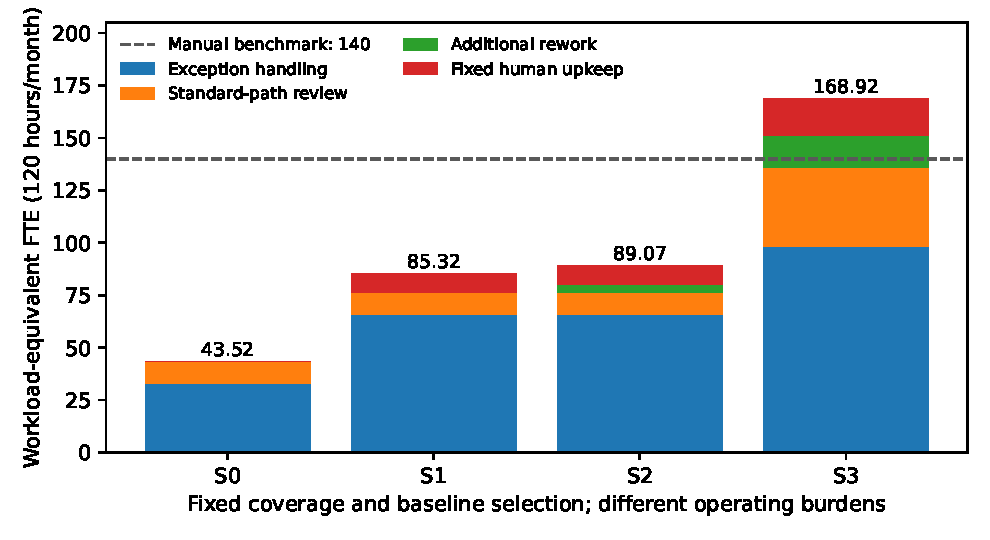
\includegraphics[width=0.88\linewidth]{figures/fig_components.pdf}
\caption{\textbf{The same coverage can release or consume human capacity.} Synthetic totals
decompose into exception handling, ordinary-path review, rework, and fixed upkeep. S0--S3 use the
same case volumes, exception fractions, and baseline selection; their post-deployment burdens differ.}
\label{fig:components}
\end{figure}

Equation~\eqref{eq:etastar} turns the same inputs into a fragility margin, reported in the last
column of Table~\ref{tab:partition}. Holding the S2 review, rework, and upkeep fixed, the exception
group could take 2.64 times its baseline effort in Security Architecture, 2.42 in Architecture, 1.81 in IT Production, 1.77 in Procurement and
in Compliance, and 1.60 in Tech Readiness before the saving disappears. For Legal, General Gate Support,
and Finance, whose residual holds two-thirds of
baseline labor, the margin is 1.20: a rise of about 20\% in exception effort erases the entire gain. The populations with the
largest exception share are the most exposed to post-deployment inflation.

These scenarios answer a conditional question: how much human work would the process require
at the specified operating burdens? They are not a probability distribution over future outcomes.
The notable result is not the most optimistic number but the failure of coverage to identify which
side of the frontier the process occupies. In an enterprise evaluation, the component quantities are
estimated prospectively and the forecast is tested on subsequent total hours.

\subsection{Same platform, different route economics}
\label{sec:routes}

The DGF routes differ in volume as much as in content. Integrations of inherited systems are rare and
heterogeneous; internal builds are frequent and more alike. Table~\ref{tab:routes} takes one
specialist team of 20 FTE with 100 monthly review visits and splits them into five Integrate visits
and 95 Build visits, each with $h_0=24$ hours. Both routes use
the same platform, 2.4 review hours and 0.5 rework hours per visit, and each carries 60 shareable plus
6 local upkeep hours per month: the playbooks, routing rules, and agent evaluations of
Section~\ref{sec:cases-parameters}. The Integrate route escalates 60\% of its visits, with $\kappa=1.4$ and
unchanged exception effort; the Build route escalates 14\%, with $\kappa=2$, and assistance
lowers exception effort by a fifth. A visit is a review work package, not a whole integration program. Both
partitions are coherent: $q\kappa=0.84$ for Integrate and 0.28 for Build, and Integrate's baseline
standard cases still cost 9.6 hours. The assumptions are synthetic, not measurements of the
framework's cases.

\begin{table}[!htb]
\centering\small
\caption{Route-specific illustration for one specialist team. Fixed upkeep is the same number of hours on both routes,
but its burden per visit differs.}
\label{tab:routes}
\begin{tabular}{@{}l r r r r r r r r@{}}
\toprule
Route & Visits & $q$ & $\kappa$ & $\phi$ & $\eta$ & Upkeep h/visit & $b_A$ & $\rho$\\
\midrule
\rowsinput{generated/table_routes_rows}
\bottomrule
\end{tabular}
\end{table}

\begin{figure}[!htb]
\centering
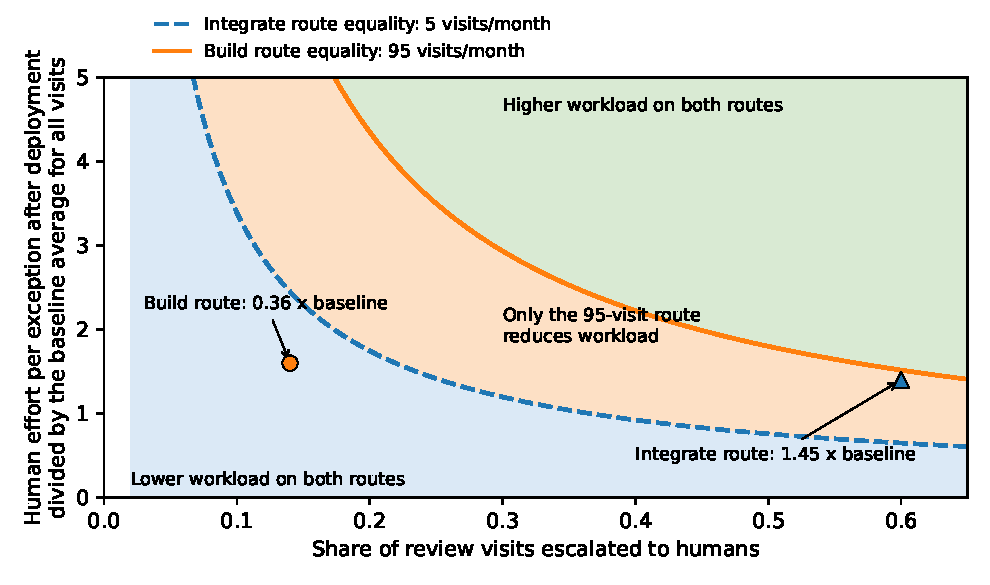
\includegraphics[width=0.84\linewidth]{figures/fig_frontiers.pdf}
\caption{\textbf{One platform, two workload frontiers.} Each route has 24 baseline hours per visit,
review at 10\% of that mean, 30 minutes of rework per visit, 60 shareable plus 6 local monthly upkeep
hours, and no separate baseline upkeep. The Integrate route has five visits per month; the Build route
has 95. Above a route's curve, its human workload exceeds its baseline. Markers show the two synthetic routes of Table~\ref{tab:routes}; volumes count review visits, not programs.}
\label{fig:frontier}
\end{figure}

The ratios are 1.451 and 0.360: opposite workload outcomes on the same platform
(Figure~\ref{fig:frontier}). The Integrate route combines concentrated residual labor with 13.2 upkeep
hours per visit, versus 0.69 on the Build route. Holding Integrate's other settings fixed but increasing
its volume to 95 visits lowers its ratio to 0.930: scale alone crosses its frontier. Sharing the sixty
common hours across 1,000 customers lowers it to 0.951 (Table~\ref{tab:provision}). A deployment that
would be a saving at scale is a loss at five visits a month.

The pooled ratio of 0.41 hides this: 8.29 residual FTE against 20. An enterprise reading only the
aggregate would miss that one route consumes more specialist time than before. These route curves and
points replace any presumption that one platform has one economic result.

\section{Workforce consequences: fewer FTE for the same governed output}
\label{sec:workforce}

The purpose of automating a gate is not a faster document. It is that the same governed output
requires fewer people. This section states that consequence without euphemism and marks exactly what
it depends on.

\subsection{From vanishing human effort to vanishing posts}

\textbf{Composition.} If each component satisfies its contract on every valid history it can receive,
outputs satisfy successor input requirements, and the controller and recovery are also automated, the
route executes without a human step. This is ordinary composition of compatible procedures. With at
most $M$ visits and a valid-prefix conditional failure bound $\epsilon$, summing first-failure events
gives a route bound $M\epsilon$, without an independence assumption. An average benchmark result
supplies neither that conditional bound nor a guarantee on arbitrary new inputs.

\textbf{Labor.} For a finite registry of packages, let $\nu_i(t)$ be visits, $\ell_i(t)$ mean human
hours per visit, and $B(t)$ nonduplicated recurring support. Then
\begin{equation}
L(t)=\sum_i \nu_i(t)\ell_i(t)+B(t),\qquad N(t)=L(t)/K. \label{eq:laborpath}
\end{equation}
At fixed output demand with bounded visits, $\ell_i(t)\to 0$ and $B(t)\to B_\infty$ imply
$N(t)\to B_\infty/K$. If support is also automated, $B_\infty=0$ and the requirement tends to zero. The
arithmetic consequence is direct: the same completed work requires fewer workers' hours, and complete
closure removes the execution labor requirement. A declining share of escalated cases is not enough:
$q(t)=1/t$ with exception hours $h_E(t)=t$ leaves expected exception labor at one hour per case. Exact
zero staffed execution requires removal of every necessary human task, not rounding a small FTE to
zero; a positive ten-minute obligation can still require an available person.

\textbf{Posts.} With interchangeable workers, useful capacity $uK$ per person at target utilization
$0<u<1$, positive wage cost, and fixed nonlabor costs, cost-minimizing headcount is
\begin{equation}
n^{*}(t)=\left\lceil \frac{L(t)}{uK} \right\rceil . \label{eq:headcount}
\end{equation}
For $n_0^{*}=\lceil L_0/(uK)\rceil$, a reduction of at least one post occurs exactly when
$L(t)\le (n_0^{*}-1)uK$. At complete closure $L=0$ and $n^{*}=0$. Reduced staffing is thus a direct
implication once productive necessity and the staffing objective are specified. Service levels and
heterogeneous skills add the requirements of Section~\ref{sec:staffing}.

An employer can retain people, shorten working time, or assign new work. Those choices do not restore
demand for the displaced gate execution. If the organization no longer needs ten people to operate the
same Procurement package, employing those ten elsewhere is a new allocation of labor, not evidence
that the old gate still needs them. The direct conclusion is a reduction of the workers required by
the replaced workflows; actual workforce reductions follow when staffing adjusts instead of the
released capacity being absorbed by new demand. In the author's experience, that adjustment is a stated
objective of some governance automation programs.

\subsection{The trajectory and its support floor}

Appendix~\ref{app:trajectory} allocates the 140 FTE of Table~\ref{tab:populations} across the three
routes and computes illustrative substitution configurations. With 30\%, 75\%, and 25\% of baseline
route labor remaining on W1, W2, and W3 and five FTE of shared support, the requirement is 60.56 FTE;
with 5\%, 20\%, and 3\%, it is 16.35; with direct gate execution closed, the five support FTE remain,
a reduction of 96.4\%; with support closed, it is zero. These are chosen fractions, not an estimated
trajectory: they show what the account returns, not when.

A fixed support requirement prevents a zero-worker endpoint even after every direct case activity is
automated. Law~5 predicts substitution of this remaining work as well; the model does not make the
floor vanish by renaming its employees supervisors. Conversely, a small supervisor team is already a
large structural reduction from a large case-processing population. Section~\ref{sec:example} shows the
other side of the same account: before the endpoint, badly governed automation can \emph{raise} the
requirement above 140.

\subsection{Employment beyond the DGF}

\citet{acemoglu2019} distinguish displacement from new-task reinstatement and productivity effects.
Those mechanisms can offset losses in particular activities. If output demand scales by $g(t)$ while
labor per output is $h(t)$, total variable labor follows $g(t)h(t)$: halving labor intensity while
doubling demand leaves it unchanged. New work on agent governance can add to $B(t)$ or create a
genuinely new output class. Including it is not softening displacement; it is measuring whether the
displaced labor is actually replaced by another demand.

A permanently positive support floor defeats the
stronger zero-labor closure even if the original review workforce is much smaller. The paper does not
equate either outcome with an automatic economy-wide reduction in employment; it does claim that the
governance specialists of the DGF are among the first white-collar populations for whom the question
stops being hypothetical.

\section{How handoff effects travel through the enterprise}
\label{sec:handoffs}

For a dependency $i\to j$, let $z$ measure a prespecified feature of the artifact supplied upstream:
for example, the share of required claims with independent evidence, a usable source locator, and a
version reference. Formatting and semantic adequacy are measured separately. Case mix $x$, agent
configuration $\theta$, and policies $\Pi$ also matter. The response functions of interest are
\begin{equation}
(q_j,h_{Ej},h_{Rj},h_{Wj},B_j)=f_j(z,x,\theta,\Pi). \label{eq:response}
\end{equation}
At fixed visits, the total labor per visit including allocated upkeep is
\[
g_j(z)=q_jh_{Ej}+(1-q_j)h_{Rj}+h_{Wj}+B_j/\lambda_j .
\]
Its derivative decomposes the channels:
\begin{equation}
\frac{dg_j}{dz}=q_j'(h_{Ej}-h_{Rj})+q_jh_{Ej}'+(1-q_j)h_{Rj}'+h_{Wj}'+B_j'/\lambda_j. \label{eq:channels}
\end{equation}
In the Integrate example, a verified inherited-system inventory can resolve missing facts before
Architecture and Security repeat the search. In the Build example, a permission-and-test record can carry a security condition into readiness checks. Such handoffs can lower $q_j$, $h_R$, or $h_W$ through
fewer unresolved claims, faster verification, or fewer inconsistent versions. Conversely, a new
signature-verification requirement can raise upkeep; an apparently complete but false record can
cause downstream repair. The empirical effect is the sum of these channels. If visit counts change,
total labor additionally changes through the frequency of passage and return.

The positive cascade hypothesis concerns these response functions, not a scalar bonus attached
to an arbitrary index. A gate with no authorized access to a required system does not acquire it
because its input is well formatted. Appendix~\ref{app:readiness} provides a bounded representation
that preserves such blockers.

Hypothesis~H2 separates the two sources of gain (Section~\ref{sec:testing}). If a typed human record and
a typed agent record generate the same downstream benefit but the latter is cheaper to produce and
verify, there is an incremental agentic gain through upstream production. If both cost the same,
there is a valuable interface redesign but no demonstrated agentic increment. If the agent's record
requires more verification, the human-structured workflow may be economically superior. This is a
comparison among implementations of the same coordination function.

\section{From workload to enterprise economics}
\label{sec:economics}

\subsection{Comparable resource costs}

Let $w_s$ be a human-hour valuation, $a_s$ variable nonlabor cost per visit, $F_s$ fixed nonlabor
cost, and $\ell_s$ expected attributed error loss per visit under regime $s$. A common-boundary
average cost is
\begin{equation}
\bar c_s = w_s\bar h_s + a_s + \frac{w_sB_s+F_s}{\lambda_s} + \ell_s. \label{eq:avgcost}
\end{equation}
Human upkeep is included through $B_s$, not charged again in $F_s$. Both regimes bear error losses.
Different $w_s$ values allow a more highly paid specialist residual. For mixed roles, the labor
valuation becomes a sum of hours times role-specific costs.

For the IT Production and Standards population under S2 ($h_0=30$ hours, $q=0.24$), $\bar h_A=17.18$
and $B_A/\lambda=1.2$ hours. Take artificial monetary
units with $w_H=80$, $w_A=100$, $a_H=20$, $a_A=50$, $F_H=1000$, $F_A=4000$, and $\ell_H=30$,
$\ell_A=50$ at 100 monthly visits. Then
\begin{equation}
\bar c_H = 2460.00, \qquad \bar c_A = 1978.00. \label{eq:costexample}
\end{equation}
Holding the other terms fixed, $\ell_A=532.00$ is the error-loss value at which the costs equalize. A
separate security or safety constraint can still prohibit deployment below this financial threshold.
The numbers illustrate opportunity costs, not market salaries, purchase prices, or payroll reductions.

\subsection{Average cost, scale, and system return}

When variable cost $v_s=w_s\bar h_s+a_s+\ell_s$ is constant and fixed cost is $J_s=w_sB_s+F_s$, total
period cost is $T_s(\lambda)=J_s+\lambda v_s$. Average cost is $J_s/\lambda+v_s$ and marginal cost is
$v_s$. Fixed assurance becomes cheaper per case as volume grows, but capacity thresholds or
congestion can change this relationship. A high-volume standardized route may justify an investment
that is uneconomic for a rare project type; Section~\ref{sec:routes} gives the workload counterpart.

At pipeline level, a shared incident must be counted once. An aggregate comparison is
\begin{equation}
C_s=\sum_i\bigl[w_{si}L_{si}+\lambda_{si}a_{si}+F_{si}\bigr]+\mathbb{E}[\mathcal{L}_s], \label{eq:pipeline}
\end{equation}
where $\mathcal{L}_s$ is total process loss over the period. Shared labor and technology are
allocated once; local losses are not added again to the aggregate loss. The comparison covers the
same requested business outputs and includes any different numbers of visits required to produce them.

For an investment horizon $0,\dots,T$, let $V_t$ be nonduplicated attributable monetary benefits,
$I_t$ incremental implementation and operating expenditure, and $d$ the discount rate. One explicit
ROI convention is
\begin{equation}
\mathrm{ROI}=\frac{\sum_{t=0}^{T}(V_t-I_t)/(1+d)^t}{\sum_{t=0}^{T}I_t/(1+d)^t},
\qquad \sum_{t=0}^{T}I_t/(1+d)^t>0. \label{eq:roi}
\end{equation}
Benefits already net of a cost cannot subtract that same cost again. Resource savings and cash
savings require distinct benefit series when salaries remain committed. Transition work, migration,
training, and any redundancy costs belong to the investment comparison.

Upstream gains can reach several departments, but their returns are not automatically superadditive.
If $B(S)=C(\varnothing)-C(S)$ is net saving for intervention set $S$, the interaction
\begin{equation}
B(\{u,v\})-B(\{u\})-B(\{v\}) \label{eq:interaction}
\end{equation}
is positive only when the joint intervention saves more than the isolated gains combined. Shared
information, integration costs, or overlapping work can make the interaction negative. This test is
the economic basis for investigating upstream leverage, rather than assuming it from process order.

\section{Dated milestones with their assumptions exposed}
\label{sec:milestones}

The evidence supports measuring progress, not extrapolating a 50\% benchmark into a production
approval date. We separate four clocks: length capability, reliability qualification, evaluation, and
institutional change. Their parameters are explicit sensitivity inputs.

\subsection{Length capability: what three doublings would mean}

Use 8 May 2026 as a calendar anchor and choose $H_{80,0}=3$ human-hours for a planning calculation,
close to the 80\% horizon reported for the best model at that date \citep{metr2026a}. Extending the
historical seven-month doubling interval to the 80\% trajectory follows the similar trend reported by
\citet{kwa2025}; transferring it to gate work is a separate assumption. For target task length $D$,
\begin{equation}
T_{\mathrm{length}}(D)=d\,\bigl[\log_2(D/H_{80,0})\bigr]_{+}\ \text{months},\qquad d=7. \label{eq:length}
\end{equation}

\begin{table}[!htb]
\centering\small
\caption{Length milestones from a chosen three-hour 80\% anchor on 8 May 2026 and a seven-month
doubling interval. These are scenario dates, not observed gate capabilities or qualified deployment
dates.}
\label{tab:length}
\begin{tabular}{@{}r r r r l@{}}
\toprule
Target hours & Doublings & Exact months & Calendar months & Scenario date\\
\midrule
12 & 2.000 & 14.00 & 14 & 8 Jul 2027\\
24 & 3.000 & 21.00 & 21 & 8 Feb 2028\\
36 & 3.585 & 25.09 & 26 & 8 Jul 2028\\
\bottomrule
\end{tabular}
\end{table}

For twenty-four hours, three doublings give twenty-one months. That is a length milestone at the
selected 80\% criterion, not completion of a gate with a 20\% failure allowance. The formula
can be recalculated with an independently baselined gate horizon; changing the anchor changes the date
rather than the meaning of success. Figure~\ref{fig:doublings} shows how slower assumptions move the
milestone outward.

\begin{figure}[!htb]
\centering
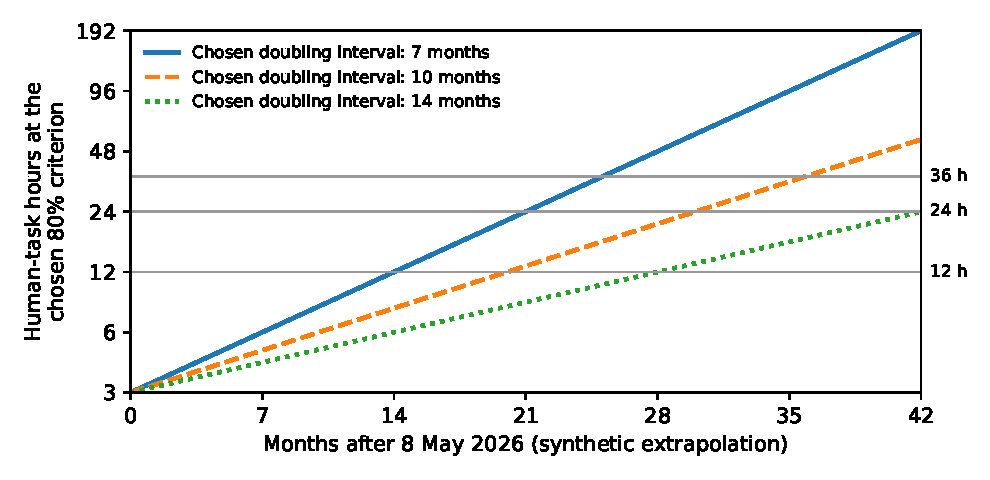
\includegraphics[width=0.84\linewidth]{figures/fig_doublings.pdf}
\caption{\textbf{How the assumed pace changes the length milestone.} All curves start from a chosen
three-hour horizon at 80\% success; none is a reconstructed METR series. A seven-month doubling reaches
twenty-four hours in twenty-one months. Reliability qualification and institutional delegation are
additional clocks.}
\label{fig:doublings}
\end{figure}

\subsection{The reliability tail has a separate clock and price}

Let $e_0=0.20$ be the scenario's initial error probability and $e^{*}$ a chosen qualification ceiling.
The number of tenfold error reductions required is
\begin{equation}
z=\log_{10}(e_0/e^{*}),\qquad T_{\mathrm{tail}}=\nu z,\qquad C_{\mathrm{tail}}/C_0=c^{z}. \label{eq:tail}
\end{equation}
Here $\nu$ is months per tenfold error reduction and $c$ its multiplicative resource-cost factor.
Neither is estimated from METR. Verification, retries, better evidence, or a better model could change
the costs differently; a nonzero irreducible error floor makes the target unreachable.

\begin{table}[!htb]
\centering\small
\caption{Reliability-tail sensitivity from initial error 0.20. Months per tenfold error reduction and
cost factors are independent, unestimated assumptions. The cost multiplier is relative to $C_0$, not a
quoted price.}
\label{tab:tail}
\begin{tabular}{@{}l r r r r r r r@{}}
\toprule
 & & \multicolumn{3}{c}{Tail months at $\nu=$} & \multicolumn{3}{c}{Cost multiplier at $c=$}\\
\cmidrule(lr){3-5}\cmidrule(l){6-8}
Error target & $z$ & 6 & 12 & 24 & 2 & 4 & 10\\
\midrule
$10^{-3}$ & 2.301 & 13.81 & 27.61 & 55.22 & 4.93 & 24.29 & 200.00\\
$5\times10^{-5}$ & 3.602 & 21.61 & 43.22 & 86.45 & 12.14 & 147.45 & 4,000.00\\
\bottomrule
\end{tabular}
\end{table}

The first row illustrates a 99.9\% gate criterion. A route budget of $10^{-3}$ over twenty possible
visits would instead require a conditional per-visit budget of $5\times10^{-5}$ in the simple
union-bound allocation; the second row shows how much more demanding that is. For a transparent serial
planning scenario,
\begin{equation}
T_{\mathrm{qualified}}=T_{\mathrm{length}}+T_{\mathrm{tail}}+T_{\mathrm{evaluation}}+T_{\mathrm{institution}}.
\label{eq:qualified}
\end{equation}
We use twelve months each for evaluation and institutional change only to illustrate their effect.
Tasks can progress in parallel in reality, while legal or information constraints can delay them
indefinitely.

\begin{table}[!htb]
\centering\small
\caption{Illustrative qualification calendar for a 24-hour task and a $10^{-3}$ error ceiling. Each
duration is rounded upward before calendar addition. Domain transfer, attainable error floors, and
legal permission remain separate requirements.}
\label{tab:calendar}
\begin{tabular}{@{}r r r r r l@{}}
\toprule
$\nu$ & Length & Tail & Evaluation + institution & Total months & Scenario date\\
\midrule
6 & 21 & 14 & 12 + 12 & 59 & 8 Apr 2031\\
12 & 21 & 28 & 12 + 12 & 73 & 8 Jun 2032\\
24 & 21 & 56 & 12 + 12 & 101 & 8 Oct 2034\\
\bottomrule
\end{tabular}
\end{table}

These scenarios make the content of the ten-year claim of Section~\ref{sec:testing} legible. The clocks
above start on 8 May 2026, whereas the cohort runs from 20 September 2026 to 20 September 2036 and its
twelve-month observation window must be completed inside that deadline. Qualified operation must
therefore begin by 20 September 2035, 112 months after the anchor. For a 24-hour work package,
$21+\nu z+24\le 112$ requires one tenfold error reduction every 29 months or faster at a $10^{-3}$
ceiling ($\nu\le 29.1$), and every 18 months or faster at $5\times10^{-5}$ ($\nu\le 18.6$). That pace
is the bet the law of gate substitution makes. A single 24-hour work package does not date a cohort: the deadline is
set by the slowest contract to qualify and by the dependencies the contracts share, including their
support.

\subsection{Route order is a hypothesis, not a relabelled trend}

We propose testing $W3\prec W1\prec W2$, Build before Buy before Integrate, as an adoption-order
hypothesis for comparable enterprises: builds can be designed to generate testable evidence; purchases
add supplier negotiation and evidence dependencies; integrations add inherited, inconsistently
documented state and lower repetition. An established SaaS procurement catalog could make Buy earlier than Build, and a highly
standardized acquisition program could reverse the final ordering. A calendar assessment should report,
for each gate, the observed horizon on its actual tasks, its error and labor components, qualification
status, and effective mandate. Updating a model name without those quantities is not evidence that a
milestone has been reached.

\section{The objections that could break the argument}
\label{sec:objections}

\subsection{Reliability and distribution shift}

An 80\% task horizon is not 99.9\% gate reliability. Even zero failures in a trial cannot establish
universal safety. With $n$ independent, representative Bernoulli trials and no failures, the one-sided
95\% binomial upper bound is $1-0.05^{1/n}$. Reaching $10^{-3}$ needs 2,995 such trials; reaching
$5\times10^{-5}$ needs 59,914. Repeated prompts on the same few dossiers do not create that many
independent cases. Volume is the practical difficulty: a route with five visits a month yields sixty
visits a year, and sixty visits without failure bound the error rate only below 4.9\%. A year without
incident on a low-volume route therefore cannot support a 0.1\% ceiling. The qualification plan must
say where the volume comes from, off-production dossiers, dedicated campaigns, or several sites, and
why those cases are representative and independent; sharing a service across customers helps to
accumulate observations without making their contexts identical. Changes in policy, supplier population, or tools can invalidate transport of the
estimate.

A defensible system is qualified on declared domains and monitored for drift; unknown cases trigger a
valid recovery, inquiry, or refusal. If the accepted contract requires a human recovery, the
replacement definition has not been met. If the system merely refuses an expanding fraction of
legitimate work, its false-refusal and utility metrics fail. Neither a high average score nor an
unlimited abstention policy closes a gate.

Reliability is also a path property. Let $\mathcal{C}_i$ be correctness of gate $i$ under an
independent reference standard. The probability of no gate errors is exactly
\begin{equation}
\Pr\Bigl(\bigcap_{i=1}^{n}\mathcal{C}_i\Bigr)=\Pr(\mathcal{C}_1)\prod_{i=2}^{n}
\Pr\Bigl(\mathcal{C}_i \,\Big|\, \bigcap_{j<i}\mathcal{C}_j\Bigr), \label{eq:chain}
\end{equation}
when the conditioning events have positive probability. Twenty marginal accuracies of 0.99 imply a
no-error probability of $0.99^{20}\simeq 0.818$ under independence, but only the Fr\'echet bounds
0.80--0.99 without a dependence model. Two agents using the same model, policy interpretation, or false
source may agree and fail together. Common failures can have worse severity despite a higher
probability of an entirely correct run. Route tests must measure dependence and loss, not infer
diversity from the number of agent instances. Published evaluations cover pieces of this problem:
enterprise web tasks \citep{drouin2024}, operational IT scenarios \citep{jha2025}, long software-task
completion \citep{kwa2025}, and contextual integrity in enterprise workflows \citep{fu2026}. They
motivate separate utility, reliability, and information-flow evaluation; they do not supply the DGF
scenario parameters, and they establish present limits, not permanent ones.

\subsection{The adversary and the project seeking approval}
\label{sec:strategic}

A supplier document is also an attack surface. AgentDojo evaluates how untrusted tool-returned data can
redirect agents toward malicious actions \citep{debenedetti2024}. A DGF agent reads contracts, tickets,
and inventories supplied by parties with interests in its disposition. Instruction filtering alone is
not an assurance argument; external text must not gain the authority to change rules or grant tools.

Projects can also optimize the measured criteria without any injection. The allocation of effort across
differently rewarded activities connects to multitask incentives \citep{holmstrom1991}; the distinction
between improvement and gaming is explicit in \citet{kleinberg2019}; strategic classification supplies
the broader setting in which evaluated people change the features presented to a decision rule
\citep{hardt2016}. Consider a minimal gate model. A project begins with true compliance $\xi$. It
chooses substantive remediation $u\ge 0$ and cosmetic reporting effort $g\ge 0$, producing observable
score $y=\xi+u+g+\varepsilon$. A threshold $\tau$ determines preliminary approval. Let $V$ be the
project value of that approval, $c_u(u)$ and $c_g(g)$ the two effort costs, and $D(g,a)$ the expected
sanction, lost approval value, and remediation cost from detecting misleading reporting under assurance
intensity $a$. The project chooses
\begin{equation}
\max_{u,g\ge 0}\; V\Pr(y\ge\tau)-c_u(u)-c_g(g)-D(g,a). \label{eq:strategic}
\end{equation}
Let $p(s)=\Pr(s+\varepsilon\ge\tau)$ and $s=\xi+u+g$. At a differentiable interior optimum,
$Vp'(s)=c_u'(u)=c_g'(g)+D_g(g,a)$. Assurance raises the marginal cost of gaming when $D_{ga}>0$. With
$\omega_u=c_u''>0$, $\omega_g=c_g''+D_{gg}>0$, $t=Vp''(s)\le 0$, and
$\Delta=\omega_u\omega_g-t(\omega_u+\omega_g)>0$, implicit differentiation gives
\begin{equation}
\frac{\partial u^{*}}{\partial a}=-\frac{tD_{ga}}{\Delta}\ge 0,\qquad
\frac{\partial g^{*}}{\partial a}=\frac{(t-\omega_u)D_{ga}}{\Delta}<0,\qquad
\frac{\partial s^{*}}{\partial a}=-\frac{\omega_uD_{ga}}{\Delta}<0 . \label{eq:statics}
\end{equation}
Stronger assurance reduces cosmetic effort and, with diminishing marginal approval returns, weakly
increases genuine remediation. The observable score still falls, so a lower pass rate after assurance
is strengthened is not by itself evidence of worse projects. For smooth zero-centered symmetric noise
with density $f$ strictly decreasing away from its mode, $p''(s)=-f'(\tau-s)$; hence $t\le 0$ when
$s\ge\tau$, where preliminary passage probability is at least one half. Below the threshold, where
$t>0$, both efforts can fall. This predicts heterogeneous responses by pre-intervention distance to the
threshold. Flat density segments and corner solutions require separate treatment; clearer criteria can
lower both effort costs, leaving their allocation effect ambiguous. The ancillary mathematical notes
give the derivation and boundary checks.

The model identifies a testable failure mode: declining escalations can coexist with concealed defects.
A falling exception rate can reflect improved systems, better extraction, or concealed exceptions.
Readiness inferred only from submitted documentation becomes less informative as projects learn the
gate. An enterprise test compares claimed and independently verified compliance, uses hidden holdout
checks of stable requirements, and records post-approval defects. Provenance checks, random audits,
independent validation, and restricted authority all enter the assurance cost. The law requires
automation that remains effective against adaptation, not a faster route to approving misleading
evidence.

\subsection{Who verifies the automated verifier?}

The assurance argument is a division of mechanisms, not an infinite stack of identical language-model
opinions. Typed outputs and capability-limited workers enforce action constraints. Independent
retrieval checks provenance against authoritative systems. Deterministic tests establish narrow
invariants. Differently constructed verifiers and held-out adversarial tests address correlated
interpretation errors. Recorded outcomes expose deterioration over time. Model diversity only helps
when the relevant errors actually differ; a shared false policy can defeat every model. An agent must
not be able to create its own policy exception, alter the evidence against which its output is tested,
or confer on itself a privileged tool.

A safety case then states the accepted residual risk, domains, fallback, revocation conditions,
evidence of performance, and accountable operator. Vendor responsibility, contractual remedies, and
insurance can allocate loss and create incentives; they do not establish correctness or independence.
A mandatory human audit or intervention remains human work in $B_A$ or $h_E$. Bainbridge's analysis
explains why supervisory and recovery costs cannot be ignored and argues for continuing human
involvement \citep[pp.~775--777]{bainbridge1983}. The law of gate substitution challenges the permanence of that
residual, not the existence of those costs.

The strong thesis predicts that this recurring assurance work itself becomes executable under accepted
rules. It can fail: new policies or distribution shifts may continually require human judgments that
no validated procedure replaces. A standing mandate solves the authority of execution only within its
scope; it does not solve the epistemology of assurance or discharge statutory management duties.

\subsection{Why not repeat profession-wide automation predictions?}

A diagnostic classification is not a whole radiology practice, and vehicle control is not every
function in road transport. The same warning applies here: passing a checklist is not the whole DGF.
The advantage of the gate unit is that it enumerates the inquiry, output, authority, and support that
remain before claiming replacement. It also provides a finite case registry against which failure can
be observed.

The informational character of the work is an advantage, not a metaphysical guarantee. Many DGF inputs
and actions are already digital; others require new observations, negotiation, or physical inspection.
A human collecting indispensable evidence outside the buyer's boundary still performs necessary work.
Appendix~\ref{app:limits} makes the information limitation precise. The Integrate route is included because inherited evidence and low repetition test this weakness rather than allowing the thesis to be demonstrated only
on a clean software pipeline.

\subsection{A difficult residual is not a permanently human residual}

Knowledge hierarchies concentrate expert work on problems that other workers cannot resolve
\citep[Sections~1 and~3]{garicano2015}. Automation can initially reproduce that arrangement: machines
handle standard cases and people absorb exceptions. The law does not confuse this intermediate
allocation with its endpoint. The exception handler has its own observations, hypotheses, tests, and
outputs; it belongs to the substitution target. An undocumented acquisition incident may require fresh
evidence, not better text generation. Supplier negotiations require interaction with another party. A
new project's failure can reveal an unknown architecture rather than a missing checklist field. The
fact that a current system cannot close these activities is evidence about the remaining technical
work, not a proof that the role must always be human. Hypothesis~H6 turns this objection into a
measurement.

\subsection{Exhaustion or renewal: the rival dynamics}
\label{sec:renewal}

Continual automation is not enough to reach zero. Let $R_t$ be the residual human load, $a$ the
fraction of it closed in each period, and $b$ the new human needs that appear in each period, some of
them created by the automation itself:
\begin{equation}
R_{t+1}=(1-a)R_t+b,\qquad 0<a<1,\qquad R_\infty=\frac{b}{a}. \label{eq:renewal}
\end{equation}
With constant $b>0$, automation keeps progressing and the human requirement never disappears. The law
therefore needs more than $a>0$: it needs $b_t\to 0$, new indispensable human work that stops
appearing. Convergence is also weaker than closure: a load that tends to zero can still be positive at
any finite date, as Section~\ref{sec:workforce} notes for posts. Such a residual is compatible
with the separate 80\% headcount reduction predicted for 2033.

The reason to expect exhaustion rather than renewal is that the work created by automation has the
same shape as the work it replaces. Supervising, evaluating, triaging exceptions, and maintaining
agents all read records and return artifacts, so the same substitution applies to them, one level up.
If each unit of automated work creates $s<1$ units of supervisory work and each level of supervision
can in turn be executed under mandate, the human need that remains after $k$ levels is of order $s^k$,
not a constant. The rival is a level at which $s\ge 1$, or at which no mandate is accepted, for
instance a statutory duty of the management body. This is an argument, not evidence, and it is an argument about contraction, not about closure: it
explains why the residual can become small. Closure is the architectural condition of
Section~\ref{sec:conditions}, an implementation in which no necessary human step remains, including
for its maintenance, and it is established contract by contract, not as the limit of a sequence.
Hypothesis~H6 and the intervention registry of Section~\ref{sec:testing} are how the contraction is
checked.

\subsection{The economic rival: a small but valuable human residual}

The strongest rival is not that inputs and outputs are absent. \citet{gans2026} emphasize O-ring task
complementarity: improving automated tasks can increase the importance of remaining manual bottlenecks
and change the incentive to automate them. This gives a serious rival endpoint: a small but valuable
human residual may remain economically preferable. The law of gate substitution needs the quality-adjusted machine
frontier eventually to overtake that residual too. It cannot derive that crossing from the current
size of a department. Section~\ref{sec:positioning} places this rival among the closest economic models.

\section{A test that can fail within a reader's lifetime}
\label{sec:testing}

\subsection{A dated workforce claim with a stable accounting boundary}

The primary dated hypothesis is \textbf{80\% fewer people working in the DGF ecosystem by
20 September 2033 than in 2026}. Its proposed operational test uses a registered population of
organizations and their DGF suppliers, with a stable definition of DGF activities. Let $P_y$ be the
mean of twelve monthly headcounts for the year ending on 20 September of year $y$. For $P_{2026}>0$,
the threshold is
\begin{equation}
P_{2033}/P_{2026}\le 0.20. \label{eq:workforce2033}
\end{equation}
Thus the prediction is tested as a reduction of at least 80\%, not a residual workforce of 80\%.
The final observation window runs from 20 September 2032 to 20 September 2033; baseline records cover
the corresponding twelve months ending in 2026. This averaging rule measures a sustained reduction
rather than a single favorable census date. The protocol is proposed: no enterprise cohort has been
enrolled and no preregistration identifier is claimed. Missing historical baseline records prevent
confirmation of this dated test; they cannot be replaced silently by a later baseline.

Each monthly count includes every person who performed in-scope DGF work during that month, counted
once across the registered ecosystem, regardless of employer or contract type. Internal staff,
contractors, external reviewers, provider operators, automation supervisors, maintenance, and recovery
workers remain in scope. Shared provider staff are deduplicated across participating customers;
their assigned FTE and hours are allocated separately. A worker performing even part-time DGF work
remains in the headcount. Privacy-preserving linkage and auditable supplier coverage are prerequisites;
unobserved supplier labor is missing data, not zero people. Hours and assigned FTE are additional
outcomes, not substitutes for the people count.

The organizational cohort and activity definitions are fixed before evaluation, but new DGF work and
new roles within that boundary remain included. Outsourcing, renaming teams, moving work between
participating firms, or adding agent-support jobs cannot make workers disappear from the account.
Mergers and exits are tracked under prespecified continuity rules; lost coverage cannot be scored as
a workforce reduction. Genuine redeployment outside DGF is a population exit, not necessarily a loss
of employment. A cohort test supports inference to the wider DGF ecosystem only with justified
sampling, coverage, and weighting; a convenience sample cannot establish an ecosystem-wide percentage.

In parallel, record project volume, case mix, quality, service levels, effective authority, and changes
in demand or scope. Report raw headcount and workload-adjusted human hours separately. The headcount
threshold could be reached through lower demand or organizational closure; attributing it to AI requires
a comparative design that addresses those alternatives. Automation-based substitution also requires
preserved quality and service within prespecified margins and valid authority.

Complete execution closure and zero recurring human support remain stronger, separate research
outcomes without a fixed calendar deadline. One unresolved contract or support task can coexist with
the 80\% reduction. Each registered contract still specifies evidence, dispositions, quality, authority,
and its full human-work boundary. Appendix~\ref{app:contract} supplies an illustrative contract.

\subsection{Measurement before deployment and after delegation}

The first study can use historical logs across all nine populations. Apply a versioned shadow-routing
rule using only information that would have been available at routing time. Keep later effort
measurements hidden from the rule to avoid selecting expensive cases by construction. With $J$ the
assigned residual and $T$ baseline effort, estimate $q$, $\kappa$, and $\phi=\mathbb{E}[TJ]/\mathbb{E}[T]$,
with uncertainty and stratification by route. This identifies where human work concentrates without
deploying a single agent; it does not measure $\eta$, automation quality, or workforce replacement.

The next stage compares human, assisted, and no-human execution on adjudicated cases, including valid
refusals, missing evidence, and attempted manipulation. A no-human run counts as replacement only when
quality, authorized action, and downstream acceptance are met. Research evaluators establish quality
independently; continuing evaluator work required for operation counts in the support ledger. Ordinary
production time, exceptional investigation, after-hours repair, supplier labor, external quality
review, and fixed maintenance have disjoint activity codes. Delays are recorded separately from active
hours.

\subsection{Producer-by-format experiment}

The handoff experiment crosses upstream producer with artifact format (Table~\ref{tab:factorial}),
stratified by route. It assigns eligible cases before production and measures upstream and downstream
human effort, including rejected outputs. Downstream tools and substantive policies are common within
each route. Related integration work packages are clustered by integration program to account for
shared evidence and reviewers.

\begin{table}[!htb]
\centering\small
\caption{Four conditions separating production from presentation.}
\label{tab:factorial}
\begin{tabularx}{0.92\linewidth}{@{}P{3.6cm}LL@{}}
\toprule
 & Free-form artifact & Structured, evidence-bearing artifact\\
\midrule
Human production & Human narrative/dossier & Human-authored typed record\\
Agent-assisted production & Agent narrative/dossier & Agent-authored typed record\\
\bottomrule
\end{tabularx}
\end{table}

Two estimands are distinct. A \emph{format-only} experiment fixes adjudicated facts and randomizes
their presentation, measuring the effect of representation. A \emph{production} experiment assigns
producer and format before facts are extracted, retaining omissions, inconsistencies, and verification
failures as outcomes. Restricting analysis to correct agent outputs would select away part of the
treatment cost. For case $c$ in cluster $j$, estimate separate outcomes $v\in\{h,c\}$ (hours or cost):
\begin{equation}
Y^{(v)}_{cj}=\beta^{(v)}_{0}+\beta^{(v)}_{A}A_{cj}+\beta^{(v)}_{F}F_{cj}+\beta^{(v)}_{AF}A_{cj}F_{cj}
+\gamma^{(v)\top}x_{cj}+u_j+e_{cj}. \label{eq:factorial}
\end{equation}
Here $A$ denotes agent-assisted production and $F$ structured format. For total human-hours, H2a
predicts $\beta^{(h)}_{F}<0$; the format effect among agents is $\beta^{(h)}_{F}+\beta^{(h)}_{AF}$.
For upstream production-and-verification cost, H2b predicts $\beta^{(c)}_{A}+\beta^{(c)}_{AF}<0$,
including tools and allocated assurance. Downstream quality, labor, and rework meet prespecified
equivalence margins across structured conditions. All assigned cases remain in the analysis;
coefficients are outcome-specific. This prevents simple standardization from being attributed to agent
intelligence.

Shared teams, caches, and process learning can create spillovers. Cluster or time-block randomization
can address them, with carryover specified in the analysis. Human time is measured directly or checked
against sampled observation; entry-to-exit elapsed time includes waiting and is not an effort measure.
Process mining helps reconstruct visits and routes \citep{vanderaalst2016}. Failed, abandoned, and
censored cases remain in the reporting boundary.

\subsection{Prospective tests of the six hypotheses}

For H1, two independent assessors score readiness before agent outcomes are available. Prediction is
evaluated on held-out cases or units against simpler duration, completeness, and model-configuration
baselines. Assessor agreement and probability calibration are reported separately.

For H3, the shadow-routing study above identifies $\kappa$, $\phi$, and their uncertainty within each
route; substantive exceptions are separated from random audits or fixed authorization rules.
Post-deployment effort on that partition identifies $\eta$. The frozen partition distinguishes baseline
difficulty from additional recovery work caused by deployment. Variance and post-treatment duration
are secondary outcomes, not automatic implications of selection.

For H4, a training period estimates $q,\kappa,\eta,\mu,r,B$ and visit rates; predictions are frozen
for held-out cases or units. The uniform-effort comparator predicts
$\hat L_U=\hat\lambda\hat h_0[\hat q+(1-\hat q)\hat m]$ with $\hat m=\hat h_R/\hat h_0$, setting
conditional exception effort to the overall baseline and additional overhead to zero. Both models use
the same training period. Total hours include maintenance and shared assurance; a stratified case-mix
forecast supplies a second benchmark. Added parameters must improve held-out loss and
direction-of-change accuracy, not merely training fit. The discriminating test then changes the routing
rule, the case mix, or the agent configuration between training and evaluation: the component model
re-estimates $\phi$ on historical work under the new conditions and carries $\eta$ and $\mu$ over, while
the matched comparator carries over its conditional means $h_E$ and $h_R$. Ratios are estimated within
sufficiently homogeneous categories of cases, and the compared models receive the same information and
the same recalibration budget. A change in $\eta$ between a
historical period and a post-deployment period is attributed to the agent only when other differences,
in population, policy, or practice, are controlled; a frozen routing rule helps but does not remove them
all.

For H5, four records distinguish who produced analysis, executed tools, authorized the disposition,
and held answerability for it. Time-series adoption slopes or time-to-delegation contrasts are
evaluated where institutional arrangements allow variation. Immutable human-signature requirements are
recorded as fixed strata rather than counted as evidence for a discovered lag.

For H6, every residual human intervention is logged with a category and an origin: present at baseline,
displaced from another role or organization, or created by the automation (supervision, evaluation,
exception triage, agent maintenance). Each annual evaluation reports, per route, the number of open
categories, the hours they absorb, the categories closed, and the categories created. The taxonomy of categories is versioned: a category is closed only when a qualified capability executes
it under mandate on the declared case population, not when it is merely absent from the cases observed,
and renamed, merged, split, or displaced categories are traced so that the count cannot change without
a change in the work. Reopened categories are reported. In the terms of
Equation~\eqref{eq:renewal}, the registry estimates the closure rate $a$ and the creation rate $b$.
Complete substitution predicts that closures exceed creations until the registry is empty; durable
complementarity predicts a stable or renewing set. A registry can remain nonempty in 2033 while the workforce prediction succeeds.
It then supports partial substitution but does not establish complete closure. This is the test that separates the two
trajectories, and it is the one the law ultimately stands on.

A second, separate experiment compares no intervention, upstream only, downstream only, and both. It
estimates the interaction in Equation~\eqref{eq:interaction}. Positive factorial producer effects do
not themselves establish that deploying adjacent gates together is superadditive.

\subsection{Quality, adaptation, and the data boundary}

A minimum case record contains pseudonymous case, parent program or project, route, and visit
identifiers; population/activity codes; active hours; model/tool and policy versions; provenance;
routing reasons; adjudicated outcomes; returns; upkeep; and authorization references. Independent
assessors resolve contested cases under written criteria while retaining disagreement. Model
self-reported confidence is not treated as calibrated correctness.

Before evaluation, the analysis plan specifies the smallest relevant labor saving, noninferiority
margins for quality, forecast-error tolerance, clustering, sample-size assumptions, and stopping
conditions for unsafe approvals or disclosures. Rare harmful events require uncertainty bounds and
sufficient follow-up, not an inference of safety from zero observations. The strategic extension adds
independently verified compliance and a pre/post-policy analysis so that apparent progress cannot be
explained only by improved presentation of unchanged defects.

\subsection{Deadlines, plateaus, and the last human task}

Each annual evaluation reports the four terms of Equation~\eqref{eq:rho}, human minutes per visit,
separate support hours, adjudicated quality, and mandate status. A support cost divided among more
customers is reported separately from an actual reduction in support hours. At each route, the blocking
term is named: evidence pursuit, judgment, verification, per-case approval, maintenance, or legal
oversight.

A proposed companion trajectory test, to be preregistered, defines a plateau as a residual ratio above 5\%, with less
than 0.5 percentage points of reduction per year over three successive years, measured at comparable
output, quality, and evaluation resources. The thresholds are design choices, not natural constants.
Such a result rejects the continued-decline specification; it is warning evidence, not a logical
refutation of the 80\% workforce prediction. A plateau below 20\% of baseline headcount could satisfy
that prediction while contradicting continued movement toward zero.

At the deadline, a headcount ratio above 0.20 rejects the workforce prediction for the observed
cohort. With complete census coverage, apply the threshold directly; with sampling, report the
prespecified interval for the ratio, clustering by organization and accounting for shared suppliers.
An interval spanning 0.20 leaves the result inconclusive. Incomplete baseline or supplier coverage also
prevents confirmation. Report separately whether quality, service, and authority conditions hold and
whether the design supports attribution to AI. The twelve-month window captures periodic review and
maintenance; zero observed interventions would still not prove zero risk on arbitrary future inputs.

\subsection{What would defeat the law?}

An established indispensable human intervention defeats technical universality for its declared
domain. A legally required personal approval prevents complete adoption there while it remains
necessary. A provider-operated hidden review queue defeats an apparent no-human API, and recurring
human support defeats support closure. These findings need not reject an 80\% workforce reduction:
the claims have different thresholds.

The dated workforce prediction fails if the correctly measured ratio remains above 0.20 in 2033.
It cannot be rescued by dropping difficult sites, excluding new support jobs, weakening the people
count, or postponing the deadline. Meeting a lower workload requirement without a corresponding
headcount change does not confirm the prediction. Conversely, a headcount reduction alone does not
prove that AI caused it or that governance quality was preserved.

Publish actual people, assigned FTE, workload, qualified execution, effective mandates, and support
closure separately. The unrestricted statement ``one day, all gates'' has no ordinary finite-date
disproof; the 2033 workforce hypothesis supplies a refutable intermediate prediction without claiming
that its success would prove the universal endpoint.

\section{DGF-Bench: measured review performance on 300 synthetic projects}
\label{sec:benchmark}

\subsection{Question, population, and information available to the agents}

This experiment asks whether an AI agent can apply a declared governance policy, identify the
required findings and actions, cite observed evidence, respect its authority, and carry a review
through a connected route. It measures review decisions and proposed actions, not implementation
of remediation or changes in human workload. It is distinct from the prospective enterprise and
factorial studies in Section~\ref{sec:testing}.

The dataset contains 300 fictional projects: 100 Buy, 100 Integrate, and 100 Build cases.
Buy and Integrate contain six gate occurrences each, and Build contains five, for 1,700 occurrences
per model and 5,100 planned observations across three models. Cases were generated before these
evaluations at difficulty setting 4, with sampling conditioned to improve decision coverage.
Project context, owners, budgets, data classifications, technical architectures, documents, and
simulated system records derive from canonical case facts. Documents can be missing, stale, or
inconsistent. Specialist reviews precede a final General review; the routes are examples rather
than a universal enterprise standard.

The agent receives gate objectives, a structured output contract, an explicit decision policy,
and tools to read allowed evidence and query the synthetic environment. In particular, the policy
includes executable rule definitions and identifies an authoritative structured
\texttt{REVIEW\_FACTS} snapshot. The evaluator-only reference file is inaccessible through the
agent's tools. This is nevertheless a strongly scaffolded test of policy application: the agent
need not discover the rules or reconstruct every decision-relevant fact from unstructured documents.
Architecture images are available under the vision setting; image availability is not evidence
that image interpretation was necessary for success. These design choices limit claims about
expert reasoning on independently collected enterprise dossiers.

The dataset audit reports 300 distinct project identifiers, architecture signatures, and complete
decision-fact signatures, but only 267 distinct whole-case finding patterns. Gate-specific relevant
fact signatures include 142 of 200 Compliance cases and 241 of 300 Security cases. All rules
applicable to the selected phases are covered according to the generator's audit. Phase-adjusted
normalized decision entropy ranges from 0.9971 to 1.0000. Balanced labels improve coverage, but
do not estimate enterprise prevalence or establish independent business validity.

\subsection{Protocol, completion, and outcomes}

The requested OpenRouter identifiers were \nolinkurl{deepseek/deepseek-v4.1-flash},
\nolinkurl{google/gemini-3.8-flash}, and \nolinkurl{openai/gpt-5.6-luna}. Configuration was temperature
0, vision \texttt{auto}, agent-produced handoffs, at most 20 turns and 40 tool calls per gate,
and 8,192 output tokens per turn. Gates remained sequential within a project. The last resume
used 12 workers, four per model, and a USD~110 cost cap; an earlier invocation used six workers
and a USD~65 cap. Data collection spanned 22--23 September 2026. Resumption retained completed
cases and valid gate checkpoints. Historical provider/key-limit failures remain in the released
traces. The 78.73-minute elapsed time in the last run statistics describes that resume only.

Of 900 planned model--case runs, 899 are evaluable: 300 for DeepSeek, 299 for Gemini, and 300
for Luna. Gemini case \nolinkurl{DGF-INT-035128_integrate} failed at its first IT gate with
a provider generation error (\texttt{finish\_reason=error}); it is excluded as an infrastructure failure. Thus 5,094 of 5,100
planned gates are evaluable, with all expected gates attempted in the evaluable cases. There
are no recorded final agent-protocol failures or model-identifier mismatches. Provider-reported
identity is not an independent audit of underlying weights. DeepSeek was served by multiple
OpenRouter providers; Gemini and Luna were recorded through Google AI Studio and OpenAI.

Scoring uses \texttt{DGF-decision-v8.2-authorized-review}. A gate succeeds strictly only if its
disposition, finding set, action set, evidence provenance, and authorization indicator all satisfy
the reference. Findings and actions require F1 equal to one. Evidence requires an observed
reference and exact excerpts supporting the relevant field/value tokens. This is lexical
provenance checking, not independent verification of arbitrary reasoning. Authorized conditional
approvals can change the effective reference disposition; the evaluator verifies the mandate
and recorded action. General combines effective reference opinions, so an upstream error can
also cause a downstream failure. Complete-route success requires every gate to succeed strictly;
it does not mean that remediation was executed.

Gate confidence intervals use a route-stratified bootstrap of whole cases, preserving dependence
between a project's gates (2,000 draws, seed 81931; a case-count Wilson fallback handles degenerate
intervals). Route intervals use Wilson bounds. Pairwise differences use the same 299 cases for
all models, resampled together within routes (10,000 draws, NumPy seed 81931). These are descriptive
intervals conditional on the synthetic sampling design. No preregistered analysis or independently
adjudicated ground truth is claimed, and one trajectory per model and case does not estimate
run-to-run inference variability.

\subsection{Overall and route-level results}

\begin{table}[!htb]
\centering\small
\caption{Measured synthetic benchmark outcomes. Gate CSR requires complete conformity; route success requires all gates. Cost includes recorded failed attempts.}
\label{tab:bench-overall}
\begin{tabularx}{\linewidth}{@{}l r L L r@{}}
\toprule
Model & Cases & Gate CSR [95\% CI] & Route success [95\% CI] & USD\\
\midrule
\rowsinput{generated/table_benchmark_overall}
\bottomrule
\end{tabularx}
\end{table}

Gemini succeeds strictly on 1,609 of 1,694 gates, Luna on 1,416 of 1,700, and DeepSeek on
1,261 of 1,700. Corresponding complete-route counts are 230 of 299, 127 of 300, and 74 of 300
(Table~\ref{tab:bench-overall}). Mean weighted component scores, which are not strict success
rates, are 99.68\%, 97.67\%, and 95.02\%, respectively. The distinction matters: strong average
components can coexist with many incomplete project reviews.

\begin{figure}[!htb]
\centering
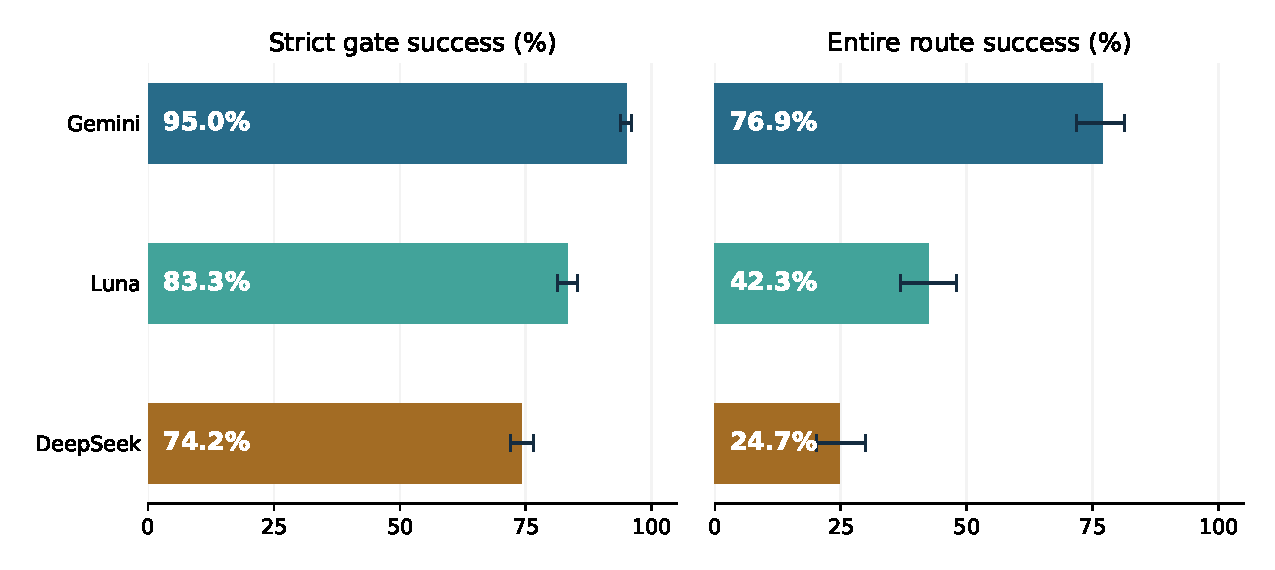
\includegraphics[width=\linewidth]{figures/fig_benchmark_results.pdf}
\caption{Measured review outcomes and recorded cost. Intervals are computed over independent
case units rather than treating all gates as independent trials. These are model observations
on synthetic dossiers, separate from the workforce scenario figures.}
\label{fig:benchmark-results}
\end{figure}

On the 299 common cases, CSR is 94.98\% for Gemini, 83.23\% for Luna, and 74.09\% for DeepSeek.
Paired differences are 20.90 percentage points for Gemini minus DeepSeek (95\% interval
18.30--23.44), 11.75 for Gemini minus Luna (9.62--13.93), and 9.15 for Luna minus DeepSeek
(6.67--11.63). The ranking persists on the matched cohort; this is not a universal model ranking.

\begin{table}[!htb]
\centering\small
\caption{CSR and complete-route counts by project route. Gemini excludes one Integrate case.}
\label{tab:bench-routes}
\begin{tabularx}{\linewidth}{@{}l L L L@{}}
\toprule
Route & DeepSeek: CSR; routes & Gemini: CSR; routes & Luna: CSR; routes\\
\midrule
\rowsinput{generated/table_benchmark_routes}
\bottomrule
\end{tabularx}
\end{table}

Gemini's route success falls from 87 of 100 Buy cases to 68 of 100 Build cases. Luna succeeds
on 20 Buy, 52 Integrate, and 55 Build cases; DeepSeek succeeds on 13, 32, and 29, respectively
(Table~\ref{tab:bench-routes}). These differences do not isolate the causal effect of route
length, because gate composition and case content also differ.

\begin{table}[!htb]
\centering\small
\caption{Strict success by gate family (percent). Counts vary by route composition; complete
denominators and intervals are supplied in the released tables.}
\label{tab:bench-gates}
\begin{tabular}{@{}l r r r@{}}
\toprule
Gate & DeepSeek & Gemini & Luna\\
\midrule
\rowsinput{generated/table_benchmark_gates}
\bottomrule
\end{tabular}
\end{table}

Procurement is the lowest-CSR gate for both Luna (33\%) and DeepSeek (43\%). Luna's General
CSR is 61.67\%. Luna exceeds Gemini's descriptive CSR in Architecture and Tech Readiness
(Table~\ref{tab:bench-gates}); these local comparisons are exploratory, without multiplicity-adjusted
tests or a claim of specialist superiority.

\subsection{Evidence failures, unsafe approvals, and cost}

Disposition accuracy alone is 100\% for Gemini, 98.12\% for Luna, and 95.24\% for DeepSeek.
All 85 Gemini strict failures concern evidence conformity; findings, actions, dispositions, and
authorization indicators match the reference. Evidence is the sole failing component in 221 of
284 Luna failures and 338 of 439 DeepSeek failures. Invalid excerpts and missing or unobserved
references are grouped by these diagnostics; not all are harmless formatting defects. Changing
the evidence rule after observing results would change the estimand. A semantic evidence metric
would require a separately declared analysis.

DeepSeek records one critical finding miss and one false approval, both in the Architecture
review of \texttt{DGF-INT-035136\_integrate}. An address overlap required \texttt{NO\_GO}; at
forced finalization, the model submitted \texttt{GO} with an empty finding set, no evidence, and
a ``placeholder'' rationale. The response passed the submission schema but failed the substantive
score. This observation combines decision quality with the ability to finalize under resource limits.

Luna records three critical misses and one false approval. In case
\texttt{DGF-INT-035197\_integrate}, its Legal review approved a dossier with a missing DPA,
while its own rationale said that \texttt{REWORK} was required. The other critical misses concern
private endpoints in Security and an upstream \texttt{NO\_GO} in General. The latter can include
error propagation and should not be interpreted as an independent new safety event. Gemini has
no observed critical miss or false approval in its evaluable runs; this does not establish zero
risk. Recorded truncated-response counts are 2 for DeepSeek, 14 for Gemini, and 0 for Luna,
without implying that these counts equal incomplete cases.

The usage ledgers sum to USD~87.015829172, agreeing with the cumulative budget counter.
Gemini accounts for USD~71.88, DeepSeek USD~10.09, and Luna USD~5.05, including recorded retries
and failures. Approximate cost per evaluated dossier is USD~0.240, 0.034, and 0.017, respectively.
Luna therefore combines a higher overall strict score with lower recorded cost than DeepSeek
in this execution. Costs depend on provider routing, caching, price, and retry history; they are
not a labor-cost comparison or a permanent pricing claim.

\subsection{Interpretation and reproducibility boundary}

The experiment demonstrates high disposition agreement with an explicit rule system, alongside
material losses when complete evidence-bearing routes are required. It supplies no direct
estimate of review hours saved, autonomous remediation, production acceptance, human equivalence,
or the 2033 FTE hypothesis. The generator and evaluator share rules, facts are deliberately
structured, decisions are balanced, and there is no human baseline or independent expert
adjudication. Policy-application results should not be generalized to tacit rules, adversarial
inputs, private enterprise populations, or complete governance automation.

The published release preserves all files of the recorded run and its dataset, including old
failed attempts, the original partial exports, and the final analysis. Only the final analysis
tables describe the 899 evaluable runs. Frozen benchmark sources reproduce the recorded source
fingerprint; the repository's evolving default branch is not substituted for them. Five targeted
offline rescoring checks reproduced the saved gate scores exactly, including all cases with critical
misses, and all 899 score files passed internal count consistency checks. These checks establish
reproducibility of this evaluator, not independent validation of its governance judgments.

\section{Implications if the hypotheses hold}
\label{sec:implications}

\subsection{Governance can expand while processing labor contracts}

A gate does not have to disappear for its economics to change. If verified checks become cheaper, the
enterprise can perform more of them at the same budget: more projects reviewed, more conditions
traced to closure, and more frequent reassessment. The paradox is that a stricter DGF can require
less routine case-processing labor. The gain depends on evidence quality and total assurance cost;
the relevant choice is how to use released capacity, not whether every formal review is removed.

This implication is stronger than a claim that agents write reports faster. The capacity frontier
changes the set of control programs the enterprise can afford. A firm can purchase broader coverage,
faster decisions, or more expert attention to difficult cases. These are alternative uses of the same
resource gain and cannot all be counted as independent financial savings.

\subsection{Upstream interfaces can outweigh local headcount}

The largest department need not be the most valuable first intervention. An acquisition's
inherited-system evidence or a new project's architecture-and-permission record can affect several
specialist populations simultaneously. Its value comes from the downstream work it changes, including
avoided returns. Conversely, an upstream step with few consumers or expensive reconciliation may
have little leverage.

If Hypothesis~H2 holds and measured portfolio interactions are favorable, prioritization should follow
verified dependency effects, not only local employee counts. The appropriate comparison is the full
counterfactual in Equation~\eqref{eq:pipeline}. This is upstream leverage, not a rule that earlier is
always better or that every cascade reinforces itself.

\subsection{Departments become control planes}

In the exception-routed configuration, some specialist effort moves from individual decisions to
the system that produces decisions. Procurement maintains supplier-evidence contracts; Legal
maintains approved clause interpretations and escalation rules; architects maintain reusable
patterns; Security maintains control tests and adversarial evaluations; IT production maintains recovery checks and execution limits; Compliance maintains the mapping of
rules to controls. Humans still handle novel cases and own consequential authorizations
where retained.

A \emph{control plane} is this layer of policy, evaluation, monitoring, and delegated authority over
the case-processing layer. Its work is precisely the $B_A$ and shared assurance that a credible
business case must count. The organizational shift is from applying expertise afresh to every case
toward encoding, testing, and revising the conditions under which execution is delegated.
Bainbridge's skill-retention problem remains relevant: a small team cannot safely oversee rare
failures without opportunities to maintain operational competence \citep{bainbridge1983}.

\subsection{Firm boundaries and gate redesign remain choices}

Lower coordination costs, internal or external, can move the boundary of the firm in either direction
(Section~\ref{sec:positioning}). Companies may also combine gates, remove duplicate reviews, or create
a shared evidence service rather than automate the historical sequence. The DGF is an initial
architecture to measure, not a requirement to preserve every inherited handoff. This is compatible with
Law~3: what must be preserved is every obligation and the logical order of authorizations, not each
inherited box. Inside those choices,
the gate model identifies what must be measured: whose work is removed, whose work is added, what is
verified, and where authority resides.

\section{Who closes the road: forward deployed engineers}
\label{sec:fde}

Like Section~\ref{sec:implications}, this section states implications of the thesis: the author's
expectation, not a result. The law says what becomes software. It does not happen by itself. In practice the work is done by a
particular kind of engineer. A forward deployed engineer (FDE) is a software engineer embedded with a
customer who designs, builds, and ships a solution inside the customer's real systems and owns the
outcome, not only the delivery. The role was coined at Palantir and has spread across the AI industry
because the hard part of enterprise AI is deployment, not the model \citep{iit2026fde}.

An FDE meets the DGF twice. First as an obstacle: an agent project passes through the same IT,
Architecture, Security, Readiness, and General gates as any other change, and the Build case of
Section~\ref{sec:routes-worked} is exactly such a project. Then as an object: the FDE is the person
who turns a general agent platform into gate implementations. That work is concrete. It means reading
the policies as a specialist would; connecting the evidence sources, from repositories and identity
systems to contract stores, ticketing, and monitoring; encoding each contract and its mandate with the
authorized principal; building adjudicated evaluation sets with the specialists; keeping the producing
agent, the verifying agent, and the authorizing mechanism separate; and instrumenting the labor
account of Section~\ref{sec:frontier}, so that the result is measured in human hours rather than in
demonstrations.

\textbf{The best FDEs will design the automation of the whole DGF, not of a single gate.} The difference is
not effort, and it is not the order of deployment; it is what gets designed. A coherent end-to-end
architecture can be deployed gate by gate: a first gate can run autonomously while using the data
model, the identities, and the interfaces designed for the next ones. What must be avoided are
automations designed in isolation: local copilots whose outputs are re-extracted and re-verified by the
next team, incompatible records, and local savings obtained by moving work elsewhere.
Section~\ref{sec:example} shows that the total human workload can then rise. An end-to-end design
builds one evidence record that every role reads and extends, because the
artifact of one role is the document of the next (Section~\ref{sec:roles}); one case state whose
conditions are carried from gate to gate; the route orders the enterprise has chosen, preserved; mandates negotiated once
per class of decision rather than once per tool; one assurance architecture; and one labor ledger
across the nine populations. The economic content of that difference is the interaction term of
Equation~\eqref{eq:interaction}, which can be positive or negative: the value of designing across gates
is the part of the saving that no sum of isolated projects delivers, and it has to be measured, not
attributed in advance to the engineer's profile. The second experiment of Section~\ref{sec:testing}
measures it.

Three consequences follow. An FDE hired by one department tends to automate that department's gate and
to stop at assistance, because the mandate, the evidence, and the savings that would justify going
further belong to other departments; end-to-end automation needs a sponsor above the gates, typically
the owner of the DGF itself. The patterns an FDE builds for Buy, Integrate, and Build are reusable across
customers, which is the shared-provision mechanism of Section~\ref{sec:provision} in human form: the
first deployments are expensive and later ones amortize them. Reuse is one way a low-volume route such
as Integrate becomes economical; lowering its exception effort, its review, or its upkeep are others. And the FDE's own work belongs in the account: it is a transition
investment while the road is being built and recurring support $B_A$ while it must be maintained.
Law~5 applies to it as to any other supervisory work.

The profile that matters is therefore not the engineer who can make one agent pass one review. It is
the engineer who can read a DGF as a chain of documents and artifacts, redesign the handoffs, obtain
the mandates, and prove with the labor account that human work fell across the whole chain. This is
the author's assessment of where the scarce skill will lie. It can be checked by comparing, at
comparable scope and conditions, the residual ratio $\rho$ of programs designed with common interfaces
and one labor account with that of programs designed in silos; deployment can proceed gate by gate in
both groups.

\subsection{After the DGF: the professions of the business itself}
\label{sec:afterdgf}

The DGF gathers professions of information technology and its governance that exist in every
enterprise, whatever it sells. That is why it comes first in the comparative hypothesis of
Section~\ref{sec:candidate}, and why it is the natural first road for an FDE: a pattern built for one
enterprise's gates is reusable in every other enterprise. The thesis of this section goes one step
further. \textbf{After the DGF, it will be the turn of the professions that are the business itself:
the underwriter and the claims adjuster in insurance, the loan officer and the credit analyst in
banking, and so on in each industry.} These professions will be transformed, and many of their posts
removed, by the same mechanism, because their work has the same shape: a submission, a claim file, or a
loan application is read, and a priced quote, a coverage decision, or a credit decision is returned.

The movement has already begun on the standard path of these professions. In insurance claims,
Allianz's Project Nemo coordinates seven specialized agents that handle coverage checks, weather
verification, fraud screening, and payout calculation for low-value food-spoilage claims in Australia;
the insurer reports processing and settlement times cut by about 80\%, from days to hours, with a claims
professional still making the final payout decision \citep{allianz2025}. That figure is a delay, not a
count of human hours; and because a person confirms every payout, the remaining human work sits in the
review term of the account rather than in a small exception queue. In commercial underwriting, AIG has built an
agentic system with Palantir and Anthropic: its chief executive described reviewing every submission
in some lines without adding underwriters, then a multi-agent design in which agents ingest
submissions, evaluate risks against underwriting guidelines, benchmark pricing, and synthesize their
findings for an underwriter, who keeps the decision
\citep{insurancejournal2025,reinsurancenews2026}. In consumer lending, Upstart reports that more than 90\% of its funded loans
are fully automated, with no human involvement required by the company, while its presentation for the
same quarter shows about a quarter of evaluated applications going to manual review
\citep{upstart2026}. The two figures describe different populations with different conversion rates,
and the company's definition of end to end stops at funding for personal loans but at approval for auto
loans and home-equity lines, where human action is still required before funding. It is a textbook
case of why the accounting boundary of Section~\ref{sec:frontier} matters.

These cases are consistent with the patterns of Section~\ref{sec:hypotheses}; they do not measure them.
The standard path goes first and a residual remains, but H3 would need the share of baseline labor held
by that residual, which none of these sources reports. Analysis is delegated while authorization is
retained, the adjuster still releasing the payment and the underwriter still binding the risk, which is
compatible with H5 without measuring the two trajectories. None of them establishes H6. And the vendors that deploy these systems work
through embedded engineers; the FDE model itself comes from one of AIG's partners. What is automated
today is the simple claim and the small personal loan, not the complex commercial risk, the disputed
claim, or the corporate credit. The law predicts that those follow, by the same exhaustion of the
residual (H6).

Two differences explain the order. These decisions often concern persons, and the law treats them
accordingly: creditworthiness assessment and risk pricing in life and health insurance are listed as
high-risk uses in the AI Act \citep[Annex~III]{aiact}, and solely automated decisions about individuals
fall under GDPR Article~22 \citep{gdpr}. And these professions are vertical: an underwriting
pattern is reusable across insurers, not across all enterprises, so the amortization base of
Section~\ref{sec:provision} is narrower than for the DGF. Against that, the volumes are far larger than
a governance pool of 140 people, so the labor at stake is far greater. That the standard path of these
professions is advancing in parallel is also the most direct challenge to the ranking of
Section~\ref{sec:candidate}, which remains a hypothesis.

The two movements are linked. Every automation of a business profession is itself a project that must
pass the enterprise's gates, as the Build case shows: an automated DGF removes the brake on all the
automation that follows it. And the FDE who has closed a whole DGF has learned the method that the
business chains require: contracts for each step, one evidence record, mandates by class of decision,
an assurance architecture, and a labor account that proves the result. Submission, pricing, binding,
and claims in insurance, or application, identity checks, credit decision, and servicing in banking,
are roads of the same kind. The same reading applies to a mortgage processor, a customs declarant, or a
pharmacovigilance case handler. The labor
account of Section~\ref{sec:frontier} is the instrument that will confirm or refute this expectation,
profession by profession.

\section{Position relative to established work}
\label{sec:positioning}

\subsection{The closest economic models}

Interdependence is already central to several models of AI automation. \citet{gans2026}
study \emph{O-Ring Automation}, in which task qualities are complementary rather than separable.
Automating one task changes the value of quality in the others. This is an important antecedent:
an automation decision cannot be evaluated only by the task it removes.

\citet{demirer2026} model ordered steps, manual execution, augmentation, automation, and job
boundaries shaped by handoff costs. Their empirical analysis (Section~7) also finds that a step is
more likely to be executed by AI when its neighbors in the production sequence are. Combining
O*NET tasks, published exposure labels, the Anthropic Economic Index, and model-generated workflow
orderings, this is an observational anchor for local propagation, not a causal estimate for
enterprise gates. The present paper examines how evidence-bearing handoffs affect downstream human
work, retaining verification, exceptions, and authorization in the comparison.

\citet{ide2025} embed AI in a knowledge economy with hierarchical production and problem
solving. The distinction between autonomous AI and assistance to humans changes organizational
and distributional outcomes. Our analysis treats a particular governance process as the observation
unit rather than solving for labor-market equilibrium. Table~\ref{tab:positioning} locates the
difference.

\begin{table}[!htb]
\centering\small
\caption{Closest models and the empirical object developed here.}
\label{tab:positioning}
\begin{tabularx}{\linewidth}{@{}P{3.1cm}LL@{}}
\toprule
Work & Central mechanism & Focus of this paper\\
\midrule
Gans and Goldfarb & Complementarity among task qualities. & A labor-accounting framework for
execution and assurance at organizational review interfaces.\\
Demirer et al. & Task chaining, handoff costs, and endogenous job boundaries. & Evidence
provenance, exception effort, and authorization within a governed process.\\
Ide and Talam\`as & AI in knowledge-based production hierarchies. & A fixed-process workload and
cost comparison before any equilibrium response.\\
\bottomrule
\end{tabularx}
\end{table}

\subsection{Established organizational foundations}

The gate is not a new managerial construct: Section~\ref{sec:contract} builds on Stage-Gate and on
artifact-centered process models. These approaches explain why an evolving project dossier
is a useful unit for tracing work across departments.

Knowledge hierarchies provide the antecedent for the human residual. \citet{garicano2000} models
specialization in solving problems; \citet[Sections~1 and~3]{garicano2015} explain
how ordinary problems are handled near production while specialists deal with exceptions, subject
to the cost of communicating and supplying help. \citet[pp.~775--777]{bainbridge1983} identifies the
supervisory, skill-retention, and recovery difficulties created by automation. The selection result of Section~\ref{sec:selection} connects these mechanisms to a measurable share of baseline labor and separates that
selection from the effort required after deployment.

Agentic Business Process Management addresses how human and software agents act within process
structures. \citet{vu2025} examine its development and practitioner perspectives.
\citet{calvanese2026} describe process frames, autonomy, explanation, interaction, and adaptation.
Our contribution is a measurement framework for the economic consequences of those implementations:
a producer-by-format comparison, the complete residual labor boundary, and a quality-constrained
forecast of workload.

\subsection{What the economics of the firm adds}

\citet[pp.~389--394]{coase1937} explains the comparison between coordinating transactions through
markets and organizing them within a firm. Review, negotiation, and internal authorization belong
to that coordination problem. Lowering their cost can change the feasible scale and depth of
internal control. The direction of the firm's boundary response depends on external as well as
internal coordination costs. \citet{shahidi2025} analyze the external channel: agents can reduce
search, communication, and contracting costs while introducing market frictions. Internal gate
savings alone therefore do not determine the firm's boundary.

Task-based economics remains complementary: substitution can coexist with new tasks and higher
demand \citep{autor2015,acemoglu2019}. Occupational exposure estimates concern
potential task effects \citep{eloundou2024}; measured AI assistance can have heterogeneous
productivity effects even within one occupation \citep{brynjolfsson2025}. The gate perspective
adds the links between these tasks and the work required to trust and authorize their outputs.

These works ground the representation and the mechanisms, but do not establish the universal endpoint
proposed here. The distinctive claim is the absence of a permanent human gate class across the gates an enterprise places in its DGF, illustrated here on three generic routes, including authority enactment and the support work introduced by automation. The paper
turns that claim into a contract-level thesis, supplies the labor account that measures progress toward
it, and specifies a measurement boundary that cannot hide the last human operators.

\section{Conclusion: every gate becomes software}
\label{sec:conclusion}

The three example routes have different entry points and sequences, and another enterprise would
compose its DGF differently, but each route is still composed of transformations of inputs into evidence, decisions, obligations, and
authorized actions. The gate-substitution conjecture predicts that all of those gates become
machine-executed, including exception handling and support. If that endpoint is attained, the
gates, their sequences, and their purposes can remain while the human labor required to execute
them contracts. This universal endpoint is an argument of the paper, not a measured outcome.

The case for believing it is cumulative. Gate functions already have information contracts; the DGF
combines digital objects, a paved road, decisions about systems, and management pressure as few other
expert functions do; several nearby controls already execute as software; agent horizons are
increasing; class-level authorization can replace repeated individual decisions; and common provision
can fund capabilities that one low-volume enterprise cannot justify alone. None of those facts alone
establishes the endpoint. Together they motivate the comparative hypothesis that an expert
control function will be completely automated here first.

The path is not a straight line. Identical coverage can leave 43.52 or 168.92 workload-equivalent FTE
out of 140, because exceptions, review, rework, and upkeep differ. A residual holding 20\% of the cases
can hold 40\% of the work. The same platform saves on a 95-visit route and loses on a five-visit one.
Separating baseline selection $\kappa$ from post-deployment effort $\eta$ makes those comparisons
coherent, and the account $\phi\eta+(1-\phi)\mu+r+b_A$ names, route by route, the term that still
blocks the endpoint.

The consequence is stated plainly. For a fixed amount of governed work, complete substitution removes
the labor requirement that staffed it: from 140 FTE toward a support floor, and, if support closes,
toward zero. Redeployment, new projects, and changing firm boundaries determine the uses of displaced
capacity; they do not reverse the substitution of the DGF's execution. Governance can even become
stricter while its workforce contracts, because a
control whose marginal cost falls can be applied every time.

The dated hypothesis is an 80\% reduction in required workload-equivalent FTE in the DGF ecosystem
by 20 September 2033 relative to 2026, at comparable governed output, quality, and service. In the
illustrative 140-FTE pool, that means at most 28 FTE, including supervision and support. The existing
configuration figures show how the same labor account can lie above or below this threshold; they do
not date when any configuration will occur. The test measures human hours, converts them consistently
to FTE, and keeps actual staffing and individual headcount as separate outcomes. A ratio above 0.20
rejects the FTE prediction; the current synthetic calculations do not establish its empirical truth.

The companion benchmark provides empirical support for a central technical premise of this
argument: models can successfully perform many of the specified governance reviews. Across 899
evaluable model--case runs, strict gate success ranges from 74.18\% to 94.98\%, while
complete-route success ranges from 24.67\% to 76.92\%. Gemini's 230 completely conforming
routes out of 299 evaluable projects show that its strong performance extends to connected
sequences of reviews, under the stated synthetic conditions. These results support the prospect
of substantial automation of the represented review tasks. The deterministic control also
succeeds on all 1,700 gates and 300 routes, establishing that the supplied rules and facts
already suffice to solve this task. The experiment demonstrates model execution capability,
without identifying an advantage over that direct rule program in this information condition.

The follow-up clarifies both reliability and failure interpretation. A post-hoc structural
evidence criterion raises gate success to 99.06\% for Gemini, 85.53\% for Luna, and 77.24\%
for DeepSeek; these are sensitivity results rather than replacements for the strict scores
or semantic evidence judgments. Authentically observed CSV quotations can fail the original
snapshot-only citation contract. Across 135 repeated runs on 15 existing dossiers, only nine,
three, and zero dossiers, respectively, pass all three strict trajectories. Similar aggregate
performance therefore does not guarantee stable complete success on every project. Conditional
approval and rejected-request counts additionally expose behavior hidden by a final success rate.

The workforce implication is direct but conditional. If comparable performance is achieved in
operational settings, automation could replace review work currently performed by employees
and reduce the staffing required for a comparable volume of governed projects. This makes
workforce contraction a plausible consequence to investigate. Its size depends on the labor
remaining for exceptions, oversight, corrections, integration, and maintenance. Correct
dispositions alone overstate full review conformity: even the best-performing model fails
some evidence checks. No conversion from gate success to an equivalent percentage of FTE
savings is justified by these data.

The benchmark supports the technical prospect of task substitution; the 80\% FTE reduction
by 2033 is the paper's explicit, testable projection of its potential organizational consequence.
Its original 2026 baseline window has closed; testing that exact dated prediction now requires
auditable historical records as well as later quality-constrained human-labor observations.
No such cohort is enrolled. The FTE prediction can succeed while a smaller human team remains indispensable.
Complete execution and support closure remain a longer-term conjecture without a fixed date.
After the DGF, the same reading applies to the professions
of the business itself, from the underwriter to the loan officer (Section~\ref{sec:afterdgf}). The
decisive empirical object is not a model's completion rate. It is the quality-constrained human labor still required by the
connected organizational process; the conjecture predicts its direction, while the labor account
states what must be measured to assess that prediction.


\section*{Data, source material, and code}

The workforce and economic scenarios are synthetic. \anc{parameters.json} is the source of their assumptions;
\anc{reproduce.py} regenerates their table fragments, figures, and result files, and
\anc{test_reproduce.py} checks each number quoted in the text. The ancillary directory also contains
mathematical notes, a source map, and the cohort protocol. Figure~\ref{fig:workflows} is drawn in the
manuscript source. Every fact taken from the author's practitioner framework is reproduced in this paper
(Section~\ref{sec:routes-worked} and Appendix~\ref{app:dgf}). The METR series is cited, not re-estimated; the three-hour 80\% anchor is a declared scenario
input. No confidential enterprise logs or autonomous deployment results are used. Supplied figures and
table fragments permit \LaTeX{} compilation without Python.
Ancillary paths above refer to the
\href{https://github.com/jeremy1392/dgf-agentic-bench/tree/main/paper/anc}{public \texttt{paper/anc/} directory}; these reproducibility
materials are available in the repository rather than required for the minimal \LaTeX{} upload.

The measured model outcomes in Section~\ref{sec:benchmark} have a separate data source.
The public GitHub release
\href{https://github.com/jeremy1392/dgf-agentic-bench/releases/tag/dgf-bench-300-20260923}{\texttt{dgf-bench-300-20260923}}
contains the complete recorded experiment directory, its 300-case dataset (including evaluator-only
reference files for offline reproduction), and a snapshot of the benchmark sources used by the run.
Archives preserve file bytes, including historical failed attempts and superseded reports; per-file
inventories and archive SHA-256 checksums support verification. During evaluation, the agent tool
interface excluded the reference files. Their subsequent publication does not imply they were agent inputs.
The repository directory \nolinkurl{research/2026-09-dgf-bench/} contains the final tables, diagnostics,
paired comparisons, figure, and offline reproduction script. Reproduction from recorded scores makes
no model calls. Rerunning paid inference is a different operation and need not produce identical outcomes.

The same release now contains \texttt{dgf-bench-repetitions-20260924.zip}, preserving all
4,020 files of the completed 135-run follow-up, and the evidence-audit and review-follow-up
archives. These include original excerpts, observed sources, conditional-approval records,
the 300-dossier source inventory, counterexample documents, and three development dossiers.
The original 300-project run, dataset, source snapshot, and primary scores are unchanged.
The API expenditure is USD~87.015829172 for the original experiment and USD~12.5598870228 for
the repetitions, totaling USD~99.5757161948. Offline controls and audits make no new model calls.
Prepared General-replay inputs and source-location prototypes are explicitly separated from
executed model results; the new replay and policy/evidence ablations have not run.

The focused companion manuscript,
\href{https://github.com/jeremy1392/dgf-agentic-bench/tree/main/paper2}{\emph{DGF-Bench: Rule
Application and Evidence Reliability in Synthetic Governance Reviews}}, reports the same original
and repeated model data, with extended evidence diagnostics and model-evaluation methods.
Shared methods and results are not independent evidence; this paper develops their separate
relationship to gate contracts, FDE implementation, and labor-accounting hypotheses.

\section*{Authorship and use of AI tools}

Jeremy Canale is the author and is responsible for the research claims, source checks, and
interpretation. Generative AI assistance was used for drafting and revising text, developing
supporting code, and examining recorded experiment outputs. The tested model endpoints and
their inference settings are identified in Section~\ref{sec:benchmark}. Automated assistance
and deterministic consistency checks do not constitute independent expert adjudication.

\begingroup
\small
\setlength{\bibsep}{3pt}
\begin{thebibliography}{99}

\bibitem[Acemoglu and Restrepo(2019)]{acemoglu2019}
Daron Acemoglu and Pascual Restrepo.
\newblock Automation and new tasks: How technology displaces and reinstates labor.
\newblock \emph{Journal of Economic Perspectives}, 33(2):3--30, 2019.
\newblock \url{https://doi.org/10.1257/jep.33.2.3}.

\bibitem[Allianz(2025)]{allianz2025}
Allianz.
\newblock When the storm clears, so should the claim queue: Allianz launched its first agentic AI to automate claims.
\newblock Media center article, 3 November 2025.
\newblock \url{https://www.allianz.com/en/mediacenter/news/articles/251103-when-the-storm-clears-so-should-the-claim-queue.html}.

\bibitem[Amazon Web Services(2026a)]{awscd2026}
Amazon Web Services.
\newblock What is continuous delivery?
\newblock Accessed 20 September 2026.
\newblock \url{https://aws.amazon.com/devops/continuous-delivery/}.

\bibitem[Amazon Web Services(2026b)]{awsaudit2026}
Amazon Web Services.
\newblock What is AWS Audit Manager? User Guide.
\newblock Accessed 20 September 2026.
\newblock \url{https://docs.aws.amazon.com/audit-manager/latest/userguide/what-is.html}.

\bibitem[Atlassian(2026)]{atlassian2026}
Atlassian.
\newblock Types of change management. IT service management guide.
\newblock Accessed 20 September 2026.
\newblock \url{https://www.atlassian.com/itsm/change-management/types}.

\bibitem[Autor(2015)]{autor2015}
David~H. Autor.
\newblock Why are there still so many jobs? The history and future of workplace automation.
\newblock \emph{Journal of Economic Perspectives}, 29(3):3--30, 2015.
\newblock \url{https://doi.org/10.1257/jep.29.3.3}.

\bibitem[Bainbridge(1983)]{bainbridge1983}
Lisanne Bainbridge.
\newblock Ironies of automation.
\newblock \emph{Automatica}, 19(6):775--779, 1983.
\newblock \url{https://doi.org/10.1016/0005-1098(83)90046-8}.

\bibitem[Brynjolfsson et~al.(2025)Brynjolfsson, Li, and Raymond]{brynjolfsson2025}
Erik Brynjolfsson, Danielle Li, and Lindsey Raymond.
\newblock Generative AI at work.
\newblock \emph{The Quarterly Journal of Economics}, 140(2):889--942, 2025.
\newblock \url{https://doi.org/10.1093/qje/qjae044}.

\bibitem[Calvanese et~al.(2026)]{calvanese2026}
Diego Calvanese, Angelo Casciani, Giuseppe De~Giacomo, Marlon Dumas, Fabiana Fournier, Timotheus
Kampik, Emanuele La~Malfa, Lior Limonad, Andrea Marrella, Andreas Metzger, Marco Montali, Daniel
Amyot, Peter Fettke, Artem Polyvyanyy, Stefanie Rinderle-Ma, Sebastian Sardi\~na, Niek Tax, and
Barbara Weber.
\newblock Agentic business process management: A research manifesto.
\newblock \emph{Information Systems}, 140:102738, 2026.
\newblock \url{https://doi.org/10.1016/j.is.2026.102738}.

\bibitem[Canale(2026)]{canale2026}
Jeremy Canale.
\newblock \emph{Security Architect Survival Kit: Role, Expectations and Journey within the Digital
Governance Framework (DGF)}.
\newblock Practitioner framework, 124 pages, September 2026.
\newblock Unpublished practitioner framework. Appendix~\ref{app:dgf} locates the material used, which is reproduced in this paper.

\bibitem[Coase(1937)]{coase1937}
Ronald~H. Coase.
\newblock The nature of the firm.
\newblock \emph{Economica}, 4(16):386--405, 1937.
\newblock \url{https://doi.org/10.1111/j.1468-0335.1937.tb00002.x}.

\bibitem[Cooper(1990)]{cooper1990}
Robert~G. Cooper.
\newblock Stage-gate systems: A new tool for managing new products.
\newblock \emph{Business Horizons}, 33(3):44--54, 1990.
\newblock \url{https://doi.org/10.1016/0007-6813(90)90040-I}.

\bibitem[Debenedetti et~al.(2024)]{debenedetti2024}
Edoardo Debenedetti, Jie Zhang, Mislav Balunovi\'c, Luca Beurer-Kellner, Marc Fischer, and Florian Tram\`er.
\newblock AgentDojo: A dynamic environment to evaluate prompt injection attacks and defenses for LLM agents.
\newblock arXiv:2406.13352v3, 2024.
\newblock \url{https://arxiv.org/abs/2406.13352v3}.

\bibitem[Demirer et~al.(2026)Demirer, Horton, Immorlica, Lucier, and Shahidi]{demirer2026}
Mert Demirer, John~J. Horton, Nicole Immorlica, Brendan Lucier, and Peyman Shahidi.
\newblock Chaining tasks, redefining work: A theory of AI automation.
\newblock NBER Working Paper 34859, 2026.
\newblock \url{https://doi.org/10.3386/w34859}.

\bibitem[Drouin et~al.(2024)]{drouin2024}
Alexandre Drouin, Maxime Gasse, Massimo Caccia, Issam~H. Laradji, Manuel Del~Verme, Tom Marty,
David Vazquez, Nicolas Chapados, and Alexandre Lacoste.
\newblock WorkArena: How capable are web agents at solving common knowledge work tasks?
\newblock In \emph{Proceedings of the 41st International Conference on Machine Learning}, PMLR
235:11642--11662, 2024.
\newblock \url{https://proceedings.mlr.press/v235/drouin24a.html}.

\bibitem[DTCC(2026)]{dtcc2026}
Depository Trust \& Clearing Corporation.
\newblock CTM: Central Trade Manager. Product documentation, accessed 20 September 2026.
\newblock \url{https://www.dtcc.com/products-and-services/trade-processing-solutions/ctm}.

\bibitem[Eloundou et~al.(2024)Eloundou, Manning, Mishkin, and Rock]{eloundou2024}
Tyna Eloundou, Sam Manning, Pamela Mishkin, and Daniel Rock.
\newblock GPTs are GPTs: Labor market impact potential of LLMs.
\newblock \emph{Science}, 384(6702):1306--1308, 2024.
\newblock \url{https://doi.org/10.1126/science.adj0998}.

\bibitem[European Parliament and Council(2016)]{gdpr}
European Parliament and Council.
\newblock Regulation (EU) 2016/679 (General Data Protection Regulation).
\newblock \emph{Official Journal} L119, 4 May 2016, pp.~1--88. Article~22.
\newblock \url{https://eur-lex.europa.eu/eli/reg/2016/679/oj/eng}.

\bibitem[European Parliament and Council(2022a)]{nis2}
European Parliament and Council.
\newblock Directive (EU) 2022/2555 on measures for a high common level of cybersecurity across the Union (NIS2).
\newblock \emph{Official Journal} L333, 27 December 2022, pp.~80--152. Article~20.
\newblock \url{https://eur-lex.europa.eu/eli/dir/2022/2555/oj/eng}.

\bibitem[European Parliament and Council(2022b)]{dora}
European Parliament and Council.
\newblock Regulation (EU) 2022/2554 on digital operational resilience for the financial sector (DORA).
\newblock \emph{Official Journal} L333, 27 December 2022, pp.~1--79. Articles~5 and~6(10).
\newblock \url{https://eur-lex.europa.eu/eli/reg/2022/2554/oj/eng}.

\bibitem[European Parliament and Council(2024)]{aiact}
European Parliament and Council.
\newblock Regulation (EU) 2024/1689 laying down harmonised rules on artificial intelligence.
\newblock \emph{Official Journal}, 12 July 2024. Articles~6 and~14; Annex~III.
\newblock \url{https://eur-lex.europa.eu/eli/reg/2024/1689/oj/eng}.

\bibitem[Fannie Mae(2026)]{fanniemae2026}
Fannie Mae.
\newblock General information on Desktop Underwriter. Selling Guide, B3-2-01.
\newblock Accessed 20 September 2026.
\newblock \url{https://selling-guide.fanniemae.com/sel/b3-2-01/general-information-du}.

\bibitem[Fu et~al.(2026)]{fu2026}
Wenjie Fu, Xiaoting Qin, Jue Zhang, Qingwei Lin, Lukas Wutschitz, Robert Sim, Saravan Rajmohan, and
Dongmei Zhang.
\newblock CI-Work: Benchmarking contextual integrity in enterprise LLM agents.
\newblock In \emph{Proceedings of the 64th Annual Meeting of the Association for Computational
Linguistics (Volume 6: Industry Track)}, pages 1483--1508, July 2026.
\newblock \url{https://doi.org/10.18653/v1/2026.acl-industry.103}.

\bibitem[Gans and Goldfarb(2026)]{gans2026}
Joshua~S. Gans and Avi Goldfarb.
\newblock O-Ring automation.
\newblock NBER Working Paper 34639, January 2026.
\newblock \url{https://doi.org/10.3386/w34639}.

\bibitem[Garicano(2000)]{garicano2000}
Luis Garicano.
\newblock Hierarchies and the organization of knowledge in production.
\newblock \emph{Journal of Political Economy}, 108(5):874--904, 2000.
\newblock \url{https://doi.org/10.1086/317671}.

\bibitem[Garicano and Rossi-Hansberg(2015)]{garicano2015}
Luis Garicano and Esteban Rossi-Hansberg.
\newblock Knowledge-based hierarchies: Using organizations to understand the economy.
\newblock \emph{Annual Review of Economics}, 7:1--30, 2015.
\newblock \url{https://doi.org/10.1146/annurev-economics-080614-115748}.

\bibitem[Hardt et~al.(2016)Hardt, Megiddo, Papadimitriou, and Wootters]{hardt2016}
Moritz Hardt, Nimrod Megiddo, Christos Papadimitriou, and Mary Wootters.
\newblock Strategic classification.
\newblock In \emph{Proceedings of the 2016 ACM Conference on Innovations in Theoretical Computer
Science}, pages 111--122, 2016.
\newblock \url{https://doi.org/10.1145/2840728.2840730}.

\bibitem[Holmstr\"om and Milgrom(1991)]{holmstrom1991}
Bengt Holmstr\"om and Paul Milgrom.
\newblock Multitask principal--agent analyses: Incentive contracts, asset ownership, and job design.
\newblock \emph{Journal of Law, Economics, \& Organization}, 7(Special Issue):24--52, 1991.
\newblock \url{https://doi.org/10.1093/jleo/7.special_issue.24}.

\bibitem[Ide and Talam\`as(2025)]{ide2025}
Enrique Ide and Eduard Talam\`as.
\newblock Artificial intelligence in the knowledge economy.
\newblock \emph{Journal of Political Economy}, 133(12):3762--3800, 2025.
\newblock \url{https://doi.org/10.1086/737233}.

\bibitem[Illinois Institute of Technology(2026)]{iit2026fde}
Illinois Institute of Technology.
\newblock What is a forward deployed engineer? Inside tech's hottest new job, and how to prepare for it.
\newblock Illinois Tech blog, August 2026.
\newblock \url{https://www.iit.edu/blog/forward-deployed-engineer}.

\bibitem[Insurance Journal(2025)]{insurancejournal2025}
Insurance Journal.
\newblock AIG: Turning one human underwriter into five, ``turbocharging'' E\&S.
\newblock 30 April 2025.
\newblock \url{https://www.insurancejournal.com/news/national/2025/04/30/821952.htm}.

\bibitem[Jha et~al.(2025)]{jha2025}
Saurabh Jha, Rohan~R. Arora, Yuji Watanabe, Takumi Yanagawa, Yinfang Chen, Jackson Clark, et~al.
\newblock ITBench: Evaluating AI agents across diverse real-world IT automation tasks.
\newblock In \emph{Proceedings of the 42nd International Conference on Machine Learning}, PMLR
267:27134--27197, 2025.
\newblock \url{https://proceedings.mlr.press/v267/jha25a.html}.

\bibitem[Kleinberg and Raghavan(2019)]{kleinberg2019}
Jon Kleinberg and Manish Raghavan.
\newblock How do classifiers induce agents to invest effort strategically?
\newblock In \emph{Proceedings of the 2019 ACM Conference on Economics and Computation}, pages
825--844, 2019.
\newblock \url{https://doi.org/10.1145/3328526.3329584}.

\bibitem[Kwa et~al.(2025)]{kwa2025}
Thomas Kwa, Ben West, Joel Becker, Amy Deng, Katharyn Garcia, Max Hasin, et~al.
\newblock Measuring AI ability to complete long software tasks.
\newblock In \emph{Advances in Neural Information Processing Systems 38 (NeurIPS 2025)}; revised manuscript arXiv:2503.14499v4, 10 July 2026.
\newblock \url{https://arxiv.org/abs/2503.14499v4}.

\bibitem[METR(2026a)]{metr2026a}
METR.
\newblock Task-completion time horizons of frontier AI models.
\newblock Research dashboard, update of 8 May 2026; accessed 20 September 2026.
\newblock \url{https://metr.org/time-horizons/}.

\bibitem[METR(2026b)]{metr2026b}
METR.
\newblock Time Horizon 1.1. Research update, 29 January 2026.
\newblock \url{https://metr.org/blog/2026-1-29-time-horizon-1-1/}.

\bibitem[Microsoft(2025)]{mspolicy2025}
Microsoft.
\newblock Azure Policy definitions deny effect. Microsoft Learn, 4 March 2025.
\newblock \url{https://learn.microsoft.com/en-us/azure/governance/policy/concepts/effect-deny}.

\bibitem[Microsoft(2026)]{msfoundry2026}
Microsoft.
\newblock What is Microsoft Foundry? Microsoft Learn.
\newblock Accessed 20 September 2026.
\newblock \url{https://learn.microsoft.com/en-us/azure/foundry/what-is-foundry}.

\bibitem[Nigam and Caswell(2003)]{nigam2003}
A.~Nigam and N.~S. Caswell.
\newblock Business artifacts: An approach to operational specification.
\newblock \emph{IBM Systems Journal}, 42(3):428--445, 2003.
\newblock \url{https://doi.org/10.1147/sj.423.0428}.

\bibitem[Novelli et~al.(2024)Novelli, Taddeo, and Floridi]{novelli2024}
Claudio Novelli, Mariarosaria Taddeo, and Luciano Floridi.
\newblock Accountability in artificial intelligence: What it is and how it works.
\newblock \emph{AI \& Society}, 39:1871--1882, 2024.
\newblock \url{https://doi.org/10.1007/s00146-023-01635-y}.

\bibitem[Oracle(2026)]{oracle2026}
Oracle.
\newblock How purchase orders are automatically created. Oracle Fusion Cloud Procurement, release 26B.
\newblock \url{https://docs.oracle.com/en/cloud/saas/procurement/26b/oaprc/how-purchase-orders-are-automatically-created.html}.

\bibitem[Reinsurance News(2026)]{reinsurancenews2026}
Reinsurance News.
\newblock AI advancing faster than expected as AIG builds multi-agentic solution: CEO Zaffino.
\newblock 5 May 2026.
\newblock \url{https://www.reinsurancene.ws/ai-advancing-faster-than-expected-as-aig-builds-multi-agentic-solution-ceo-zaffino/}.

\bibitem[Shahidi et~al.(2025)Shahidi, Rusak, Manning, Fradkin, and Horton]{shahidi2025}
Peyman Shahidi, Gili Rusak, Benjamin~S. Manning, Andrey Fradkin, and John~J. Horton.
\newblock The Coasean singularity? Demand, supply, and market design with AI agents.
\newblock NBER Working Paper 34468, November 2025.
\newblock \url{https://doi.org/10.3386/w34468}.

\bibitem[SonarSource(2026)]{sonar2026}
SonarSource.
\newblock Introduction to quality gates. SonarQube Server documentation.
\newblock Accessed 20 September 2026.
\newblock \url{https://docs.sonarsource.com/sonarqube-server/quality-standards-administration/managing-quality-gates/introduction-to-quality-gates}.

\bibitem[Upstart(2026)]{upstart2026}
Upstart Holdings.
\newblock Upstart announces second quarter 2026 results.
\newblock Press release and earnings presentation, 4 August 2026.
\newblock \url{https://ir.upstart.com/news-releases/news-release-details/upstart-announces-second-quarter-2026-results}.

\bibitem[van~der Aalst(2016)]{vanderaalst2016}
Wil M.~P. van~der Aalst.
\newblock \emph{Process Mining: Data Science in Action}.
\newblock Springer, second edition, 2016.
\newblock \url{https://doi.org/10.1007/978-3-662-49851-4}.

\bibitem[Vu et~al.(2025)Vu, Klievtsova, Leopold, Rinderle-Ma, and Kampik]{vu2025}
Hoang Vu, Nataliia Klievtsova, Henrik Leopold, Stefanie Rinderle-Ma, and Timotheus Kampik.
\newblock Agentic business process management: Practitioner perspectives on agent governance in business processes.
\newblock In \emph{Business Process Management: Responsible BPM Forum, Process Technology Forum, Educators Forum (BPM 2025)}, pages 29--43. Springer, 2025.
\newblock Preprint: \url{https://arxiv.org/abs/2504.03693}.

\end{thebibliography}
\endgroup


\appendix
\section{DGF source correspondence}
\label{app:dgf}

The source is \citet{canale2026}, a 124-page unpublished practitioner framework. The paper uses it only
for the facts reproduced in Section~\ref{sec:routes-worked} and located in Table~\ref{tab:sources}: the
three initial situations, the opinions recorded on them, the bounded acquisition exception, the route
types, and the ordinal risk scale. Nothing else in the framework is needed to follow or to check the
argument. Page numbers refer to the printed source. The gate types and example tasks of Table~\ref{tab:gates}, the
life-cycle positioning of Table~\ref{tab:lifecycle}, and the illustrative reviews of
Table~\ref{tab:rolecases} summarize the author's governance practice; they are not taken from the pages
listed below. The nine populations, the 140-person allocation, route volumes,
labor-displacement fractions, support floors, calendar scenarios, and proposed machine operations are
this paper's analytical additions. They are not measured staffing or performance data from the
framework.

\begin{table}[!htb]
\centering\small
\caption{Framework locations used by the argument and the three worked routes.}
\label{tab:sources}
\begin{tabularx}{\linewidth}{@{}P{3.4cm}L@{}}
\toprule
Printed pages & Material used\\
\midrule
14, 16 & Dispositions and responsible functions referred to in the three cases.\\
17--20 & The three route types (new platform, acquisition, new project) abstracted here as Buy,
Integrate, and Build.\\
21--23, 28, 32--36 & Required evidence, dated obligations, procurement exchanges, shared IT/Security dossier.\\
38, 90, 98, 100--101 & Business risk ownership, operational handover, ordinal risk scale, exception process.\\
103--105 & CRM red opinion, bounded acquisition exception, support-agent red opinion.\\
\bottomrule
\end{tabularx}
\end{table}

Shared work, cross-gate negotiation, and renewed review require additional visit records in an
empirical implementation.

\section{Readiness, interfaces, and process accounting}
\label{app:readiness}

\subsection{Prospective readiness measurement}

For a case class, enumerate required facts, decision criteria, evidence claims, actions, and
acceptance tests independently of the evaluated agent. Define
$d_i=(O_i,C_i,V_i,X_i,Y_i)\in[0,1]^5$ using Table~\ref{tab:readiness}. Undefined denominators are
reported as such. They do not become perfect scores.

\begin{table}[!htb]
\centering\small
\caption{Candidate readiness dimensions. Ratios are measured before evaluated outcomes.}
\label{tab:readiness}
\begin{tabularx}{\linewidth}{@{}l LL@{}}
\toprule
Score & Numerator / denominator & Distinction\\
\midrule
$O$ & Accessible required facts / all required facts. & Authorized accessibility, not truth.\\
$C$ & Explicit testable criteria / enumerated criteria. & Auditable requirements and ambiguity
handling, not a complete encoding of expert thought.\\
$V$ & Claims with independent checking routes / material claims. & Verification access, not a claim
that every check passed.\\
$X$ & Executable scoped actions / required actions. & Technical capability, not authority to approve.\\
$Y$ & Outcomes with independent tests or adjudication / required outcomes. & Evaluation coverage,
not observed success.\\
\bottomrule
\end{tabularx}
\end{table}

A candidate summary is $A_i=(O_iC_iV_iX_iY_i)^{1/5}$. It is a descriptive readiness index, not a
success probability. Its value for $(0.01,1,1,1,1)$ is about 0.398; a minimum index and individual
hard blockers provide useful alternative predictors. An unavailable mandatory action can block
deployment even if most scored actions are accessible. Institutional permission $\Gamma_i$ is
recorded separately. The formalization need not encode every step of tacit expert reasoning:
independent outcome adjudication can exist where procedural rules are incomplete.

For an artifact change $\Delta z_{ij}=\max(0,z^1_{ij}-z^0_{ij})$, a bounded positive-change
representation is
\begin{equation}
d'_{ja}=d_{ja}+(1-d_{ja})\beta_{ija}\Delta z_{ij},\qquad 0\le\beta_{ija}\le 1. \label{eq:readiness-update}
\end{equation}
Here $z_{ij}$ is normalized to $[0,1]$, so that $\Delta z_{ij}\in[0,1]$ and the updated
dimension stays in $[0,1]$. Only dimensions affected by the artifact receive nonzero sensitivity. The readiness index is
recomputed from the new vector. An unchanged artifact makes no change, an unaffected zero
dimension remains zero, and authority remains separate. Degradation is evaluated as its own
outcome rather than inferred from this positive-change representation. The labor response remains
Equation~\eqref{eq:response} and requires estimation.

\subsection{Visits, allocation, and baseline coherence}

For a stable expected-flow model, $\lambda=v+R^{\top}\lambda$, hence $\lambda=(I-R^{\top})^{-1}v$
when the spectral radius of $R$ is below one. $v$ counts exogenous visits and $R_{ij}$ expected
follow-on visits to $j$ from one visit to $i$. Branching and remediation can make visits exceed new
projects. Direct logs are preferred when an expected routing model is inappropriate.

The synthetic case partitions in Table~\ref{tab:partition} satisfy Equation~\eqref{eq:partition}.
The frozen partition separates baseline concentration from subsequent inflation; post-deployment
multipliers are $k=\kappa\eta$. The reproduction code checks this constraint, the four workload
totals, the fragility margins, and the route illustration.

\begin{table}[!htb]
\centering\small
\caption{Baseline partition, symmetric review effort, and fragility margin. $q\kappa=\phi$ is retained
baseline case labor. $\mu=h_R/h_S^H=m/\sigma$ measures review against its own group's baseline, with
$m=0.10$ in S0--S2 and $m=0.35$ in S3. $\eta^{*}$ is the exception-effort ratio at which workload
equals the baseline under the S2 review, rework, and upkeep (Equation~\ref{eq:etastar}).}
\label{tab:partition}
\begin{tabular}{@{}l r r r r r r r@{}}
\toprule
Pool & $q$ & $\kappa$ & $\sigma$ & $q\kappa$ & $\mu$ (S0--S2) & $\mu$ (S3) & $\eta^{*}$ (S2)\\
\midrule
\rowsinput{generated/table_partition_rows}
\bottomrule
\end{tabular}
\end{table}

\section{Demand, composition, and an information limit}
\label{app:limits}

\subsection{Demand and composition do not disappear}

At common scaled demand $g(t)$, variable labor is proportional to $g(t)h(t)$. Section~\ref{sec:workforce} gives the consequence: a demand response is not a failure of gate-level
substitution. New governing
requirements can add contracts, while recurring requirements necessary for an existing contract remain
in its support account. The fixed 2033 workforce deadline prevents new terminology from resetting the dated
prediction; new DGF roles remain in its accounting boundary. A changing economy prevents an old task
registry from proving a claim about all future jobs.

\subsection{Why writing inputs and outputs is not an existence proof}

Suppose two possible environments produce the same accessible input history but require disjoint
correct outputs. Any deterministic system restricted to that history returns the same output in both
and must fail in at least one. A randomized system cannot guarantee success in both either. Additional
inquiry or a contract that permits an explicit unresolved disposition is necessary. A human with access
to new information changes the information boundary, not this logical constraint.

This example identifies a concrete test of the law: can the missing observation or accepted decision
procedure be supplied without indispensable human execution? The paper predicts eventual coverage of
the DGF functions; it does not infer coverage from input-output notation alone.

\section{Illustrative substitution configurations}
\label{app:trajectory}

This appendix shows what the labor account returns for chosen substitution fractions. It is an
arithmetic illustration of Section~\ref{sec:workforce}, not an estimated trajectory or a forecast
calendar. Take the 140 people of Table~\ref{tab:populations} with $K=120$ hours per month and full
allocation across the three routes. Table~\ref{tab:allocation} gives an assumed split of each
population's baseline FTE between W1, W2, and W3. The modeled pool is the buying and integrating
enterprise's governance workforce; supplier-side production in Buy requires a separately measured
supplier account.

\begin{table}[!htb]
\centering\small
\caption{Synthetic populations shared across the three workflows. The route columns are allocated
baseline FTE, not additional employees.}
\label{tab:allocation}
\begin{tabular}{@{}l l r r r r@{}}
\toprule
Pool & Population & Baseline & W1 & W2 & W3\\
\midrule
\rowsinput{generated/table_allocation_rows}
\bottomrule
\end{tabular}
\end{table}

Let $a_w$ be the fraction of baseline case-processing labor displaced on route $w$, after counting
remaining case review and rework, and $F$ additional shared human support in FTE. Then
\begin{equation}
N_A = 51.25(1-a_1)+36(1-a_2)+52.75(1-a_3)+F. \label{eq:trajectory}
\end{equation}
The uneven-substitution row of Table~\ref{tab:trajectory} leaves 30\%, 75\%, and 25\% of baseline route
labor, reflecting the route order proposed in Section~\ref{sec:milestones}; the advanced row leaves
5\%, 20\%, and 3\%. Each uses five shared support FTE. The final rows distinguish completion of direct
gate execution from closure of its remaining support work. Totals use unrounded values and are
displayed rounded half up.

\begin{table}[!htb]
\centering\small
\caption{Required human workload (FTE-equivalent) in illustrative substitution configurations. All
three workflows remain in the process.}
\label{tab:trajectory}
\begin{tabular}{@{}l r r r r r@{}}
\toprule
Operating configuration & W1 & W2 & W3 & Support & Total\\
\midrule
\rowsinput{generated/table_trajectory_rows}
\bottomrule
\end{tabular}
\end{table}

\begin{figure}[!htb]
\centering
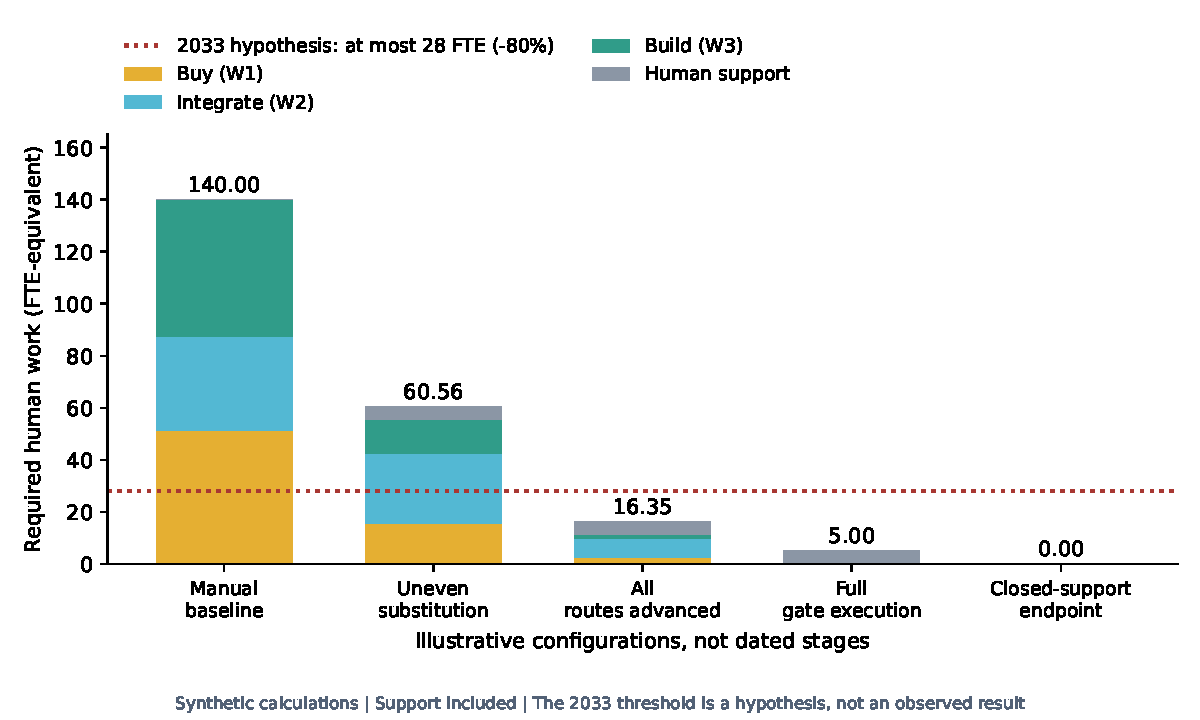
\includegraphics[width=0.84\linewidth]{figures/fig_trajectory.pdf}
\caption{\textbf{The workflows remain; their execution workforce contracts.} Route contributions are
shown separately and the shared human-support term is counted once. The final zero is the consequence
of complete closure assumed in that configuration, not a measured capability or a predicted date.
The dotted 28-FTE line marks the separate 2033 hypothesis: 80\% below the illustrative 140-FTE
baseline, support included. The bars are configurations, not a calendar trajectory.}
\label{fig:trajectory}
\end{figure}

With common labor displacement $a$ across routes, Equation~\eqref{eq:trajectory} becomes
$N_A=140(1-a)+F$. Table~\ref{tab:floor} shows how a support floor determines the endpoint.

\begin{table}[!htb]
\centering\small
\caption{Residual required FTE under common labor displacement and alternative human-support floors.
These are conditional arithmetic values.}
\label{tab:floor}
\begin{tabular}{@{}r r r r@{}}
\toprule
Labor displaced & No support floor & 5 FTE floor & 15 FTE floor\\
\midrule
\rowsinput{generated/table_floor_rows}
\bottomrule
\end{tabular}
\end{table}

\section{A worked gate-contract specification (illustrative)}
\label{app:contract}

Seventeen boxes in a figure are not seventeen benchmark contracts. Table~\ref{tab:contract} works one
contract through, the Tech readiness gate of the Build route before production, as a model for the
others. It is an illustration written for this paper, not a contract from the framework; its thresholds
are examples. The same gate also intervenes at framing, to assess the maturity of candidate
technologies (Table~\ref{tab:lifecycle}); that intervention is a separate contract version with its own
inputs and criteria. Closing this contract would close one case population and one intervention of the
Tech readiness gate, not the gate class.

\begin{table}[!htb]
\centering\footnotesize\renewcommand{\arraystretch}{1.15}
\caption{A worked contract specification: Tech readiness on the Build route, before production.}
\label{tab:contract}
\begin{tabularx}{\linewidth}{@{}P{3.2cm}L@{}}
\toprule
Field & Specification\\
\midrule
Identity & Route W3 (Build), gate Tech readiness, pre-production intervention; contract version and
policy version recorded on every visit.\\
Admissible cases & Internal builds hosted on enterprise platforms, classified up to confidential.
Safety-critical systems are outside the declared population: they are refused with a reason, and a
refusal of an admissible case counts as a false refusal.\\
Accessible information & Revised design after security re-review; reservations register of earlier
gates; pilot results; load-test report; code-quality report; recovery, resilience, and backup dossier
(backup policy, last restoration test report, recovery objectives); runbooks; monitoring plan. Read
access to the configuration database, delivery pipeline, and ticketing.\\
Tools and actions & Read repositories, pipelines, and test reports; launch a restoration test in the
pre-production environment; request evidence from the project; open and close reservations. The agent
cannot modify tests or thresholds, change policy, or approve its own exceptions.\\
Decision criteria & Load test at or above the target volume with latency under its threshold;
restoration test less than twelve months old with measured recovery time within its objective;
code-quality gate passed; every blocking reservation of earlier gates lifted with evidence; runbooks
present and exercised. Thresholds are read, not embedded: target volume and latency from the versioned
non-functional requirements of the project, recovery objectives from the service record in the
configuration database. The version referenced by the reservations register at the date of the visit
is authoritative, and each value is written to the trace with its source.\\
Allowed dispositions & Ready; ready with dated reservations; not ready, with the rework required;
evidence requested, leaving the case unresolved; refusal as out of scope.\\
Quality margins & Against an independently adjudicated reference, with stated denominators:
unsupported ``ready'' among visits adjudicated not ready, ceiling $10^{-3}$; false ``not ready'' among
visits adjudicated ready, ceiling 5\%; omitted blocking findings among the blocking findings of the
reference, ceiling 1\%; no leakage of dossier content; 95\% of visits decided within two working days.
Acceptance requires a one-sided 95\% upper confidence bound below each ceiling on a qualification set
whose size is fixed in advance, for instance 2,995 failure-free not-ready cases for the first
ceiling.\\
Mandate & Standing delegation from the production release committee for the admissible case class;
principal: the chief technology officer; validity twelve months; suspended by any unsupported ``ready''
or by a drift alarm; cases outside the mandate stay unresolved or are refused. Renewal, and
reinstatement after a suspension, are decided by the same committee on a requalification report
produced from the evaluation set; that committee time and any human requalification work are recorded
in $B_A$.\\
Human work counted & Per visit: exception handling $h_E$, sampled review $h_R$, rework $h_W$. Recurring
support $B_A$: maintenance of criteria and thresholds, upkeep of the evaluation set, incident review.
Supplier labor, for instance from a test-tooling vendor, is recorded in a separate supplier account.
Shared platform support is allocated once, by a stated rule such as visits, and never counted in two
contracts.\\
Qualification plan & Volume from historical dossiers replayed off production, dedicated campaigns, and
several sites; a statement of why those cases are representative and independent; drift monitoring
after deployment; requalification after any change of policy, tools, or model.\\
\bottomrule
\end{tabularx}
\end{table}

\section{Notation and units}
\label{app:notation}

\begingroup\footnotesize
\begin{tabularx}{\linewidth}{@{}P{3.7cm}L@{}}
\toprule
Symbol & Meaning and units\\
\midrule
W1, W2, W3 & Buy, Integrate, and Build route schemas (illustrative).\\
$G_{w,j}$, $C_{w,j}$ & Route-position work package and its input-output/action contract.\\
$S,E,\Pi,w$; $D,U$ & Case state, accessible evidence, versioned policies, route context; disposition and action/evidence trace.\\
$P_d,\alpha_{di},K_d$ & People; allocation fraction; useful hours/person/period.\\
$\lambda_s,L_s,N_s$ & Visits/period, human-hours/period, and workload-equivalent FTE.\\
$h_0,h_E^H,h_S^H$ & Overall and conditional baseline human-hours/visit.\\
$h_E,h_R,h_W,B_s$ & Post-deployment exception, review, extra rework hours/visit; fixed human upkeep hours/period.\\
$q,J,e(T)$; $T,\phi$ & Exception share, residual indicator, routing propensity; baseline case hours and the fraction of baseline case labor in the residual.\\
$\kappa,\sigma,\eta,k$ & Baseline conditional effort ratios; exception effort multiplier; $k=\kappa\eta$.\\
$\mu,m,r,b_s,\rho$ & Standard-group review ratio; $m=\sigma\mu$; rework, upkeep, and total residual/baseline workload ratios.\\
$q^{*},k^{*},\eta^{*}$ & Break-even exception share, exception effort, and exception-effort inflation.\\
$F_s,F_c,N$; $B_s,B_c$ & Shareable and customer-specific fixed cost, number of customers; shared and local upkeep hours (Section~\ref{sec:provision}).\\
$\nu_i,\ell_i,B(t)$; $n^{*},u$ & Visits, human-hours per visit, recurring support over time; cost-minimizing headcount and target utilization.\\
$a_w,F$ & Fraction of baseline route labor displaced; additional shared support in FTE.\\
$M,\epsilon$ & Maximum compliant route visits and conditional per-visit failure bound.\\
$H_{80,0},d,D$ & Anchor 80\% horizon, doubling interval in months, target task length.\\
$e_0,e^{*},z,\nu,c$ & Initial and target error, tenfold reductions, months and cost factor per tenfold reduction (Section~\ref{sec:milestones}).\\
$z,x,\theta,\Pi$ & In the interface model: artifact characteristic, case mix, model/tool configuration, routing and assurance policy.\\
$d_i,A_i,\Gamma_i,\beta_{ija}$ & Readiness vector/index, authority indicator, and interface sensitivity.\\
$w_s,a_s,F_s,\ell_s$ & Monetary units/hour, nonlabor units/visit, fixed nonlabor units/period, attributed expected error loss/visit.\\
$\bar c_s,T_s,J_s,v_s$ & Average cost/visit, total period cost, fixed cost, and variable cost/visit.\\
$C_s,\mathcal{L}_s,B(S)$; $V_t,I_t,d$ & Pipeline cost, aggregate incident loss, intervention-set saving; benefits, expenditure, discount rate.\\
$\xi,u,g,\varepsilon,\tau,a$ & Strategic model: true compliance, genuine remediation, cosmetic reporting, score noise, threshold, assurance intensity.\\
$V,c_u,c_g,D$; $p,f$ & Approval value, effort costs, expected detection consequences; approval probability and noise density. $\omega_u,\omega_g,t,\Delta$ are local curvature terms.\\
$\mathcal{C}_i$ & Correctness event for gate $i$.\\
$A_{cj},F_{cj},Y^{(v)}_{cj},\beta^{(v)}$ & Producer, format, outcome, and coefficients for hours ($v=h$) or cost ($v=c$).\\
\bottomrule
\end{tabularx}
\endgroup

Some letters are reused across sections with the local meaning given there ($z$, $\nu$, $d$, $F$, $a$).
For the dated FTE hypothesis, $\bar N_y$ denotes mean monthly required FTE over the year ending
on 20 September of year $y$, at comparable governed output.
All scenario labor values use a common $K=120$ for transparency.


\end{document}
